%
% This is a borrowed LaTeX template file for lecture notes for CS267,
% Applications of Parallel Computing, UCBerkeley EECS Department.
% Now being used for CMU's 10725 Fall 2012 Optimization course
% taught by Geoff Gordon and Ryan Tibshirani.  When preparing 
% LaTeX notes for this class, please use this template.
%
% To familiarize yourself with this template, the body contains
% some examples of its use.  Look them over.  Then you can
% run LaTeX on this file.  After you have LaTeXed this file then
% you can look over the result either by printing it out with
% dvips or using xdvi. "pdflatex template.tex" should also work.
%
\documentclass[twoside]{article}
\usepackage{graphicx}
\usepackage{tikz}
\usepackage{mathpazo}
\usepackage{hyperref}
\usepackage{sidecap}
\usepackage[version=4]{mhchem}


\usetikzlibrary{decorations.pathmorphing}
\hypersetup{colorlinks=true, citecolor=blue, filecolor=blue, linkcolor=blue, urlcolor=blue}
\setlength{\oddsidemargin}{0.25 in}
\setlength{\evensidemargin}{-0.25 in}
\setlength{\topmargin}{-0.6 in}
\setlength{\textwidth}{6.5 in}
\setlength{\textheight}{8.5 in}
\setlength{\headsep}{0.75 in}
\setlength{\parindent}{0 in}
\setlength{\parskip}{0.1 in}
%
% ADD PACKAGES here:
%
\usepackage{amsmath,amsfonts,graphicx}
%
% The following commands set up the lecnum (lecture number)
% counter and make various numbering schemes work relative
% to the lecture number.
%
\newcounter{lecnum}
\renewcommand{\thepage}{\thelecnum-\arabic{page}}
\renewcommand{\thesection}{\thelecnum.\arabic{section}}
\renewcommand{\theequation}{\thelecnum.\arabic{equation}}
\renewcommand{\thefigure}{\thelecnum.\arabic{figure}}
\renewcommand{\thetable}{\thelecnum.\arabic{table}}
%
% The following macro is used to generate the header.
%
\newcommand{\lecture}[4]{
   \pagestyle{myheadings}
   \thispagestyle{plain}
   \newpage
   \setcounter{lecnum}{#1}
   \setcounter{page}{1}
   \setcounter{section}{0}
   \setcounter{equation}{0}
   \setcounter{figure}{0}
   \noindent
   \begin{center}
   \framebox{
      \vbox{\vspace{2mm}
    \hbox to 6.28in { {\bf Physics 467/667: Thermal Physics
	\hfill Spring 2019} }
       \vspace{4mm}
       \hbox to 6.28in { {\Large \hfill Lecture #1: #2  \hfill} }
       \vspace{2mm}
       \hbox to 6.28in { {\it Lecturer: #3 \hfill Scribes: #4} }
      \vspace{2mm}}
   }
   \end{center}
   \markboth{Lecture #1: #2}{Lecture #1: #2}
   \vspace*{4mm}
}

\renewcommand{\cite}[1]{[#1]}
\def\beginrefs{\begin{list}%
        {[\arabic{equation}]}{\usecounter{equation}
         \setlength{\leftmargin}{2.0truecm}\setlength{\labelsep}{0.4truecm}%
         \setlength{\labelwidth}{1.6truecm}}}
\def\endrefs{\end{list}}
\def\bibentry#1{\item[\hbox{[#1]}]}
%Use this command for a figure; it puts a figure in wherever you want it.
%usage: \fig{NUMBER}{SPACE-IN-INCHES}{CAPTION}
\newcommand{\fig}[3]{
			\vspace{#2}
			\begin{center}
			Figure \thelecnum.#1:~#3
			\end{center}
	}
% Use these for theorems, lemmas, proofs, etc.
\newtheorem{theorem}{Theorem}[lecnum]
\newtheorem{lemma}[theorem]{Lemma}
\newtheorem{proposition}[theorem]{Proposition}
\newtheorem{claim}[theorem]{Claim}
\newtheorem{corollary}[theorem]{Corollary}
\newtheorem{definition}[theorem]{Definition}
\newenvironment{proof}{{\bf Proof:}}{\hfill\rule{2mm}{2mm}}
% **** IF YOU WANT TO DEFINE ADDITIONAL MACROS FOR YOURSELF, PUT THEM HERE:
\newcommand\E{\mathbb{E}}

\begin{document}
% This syllabus template was created by:
% Qiang Zhu
% Document settings
%\documentclass[11pt]{article}
%\usepackage[margin=1in]{geometry}
%\usepackage[pdftex]{graphicx}
%\usepackage{multirow}
%\usepackage{setspace}
%\usepackage{hyperref}
%\usepackage{breakurl}
%\pagestyle{plain}
%\setlength\parindent{0pt}
%\def\UrlBigBreaks{\do\/\do-\do:}
%\begin{document}
% Course information
\begin{tabular}{ l }
  \LARGE Physics 467/667 (Spring 2019)\\
  \LARGE Thermodynamics/Statistical Physics \\
  \LARGE Tues/Thurs 11:30AM - 12:45PM BPB 249 \\
\end{tabular}\\\\
%\vspace{10mm}

% Professor information
\begin{tabular}{ l l }
  \large Instructor &\large Prof. Qiang Zhu \\
  \large Email      &\large qiang.zhu@unlv.edu \\
  %\large Website    &\large \url{http://www.physics.unlv.edu/~qzhu/} \\
  \large Office     &\large BPB 232 \\
  \large Office hrs &\large Tue/Thurs 10:00AM - 11:30AM \\
\end{tabular}\\

%\vspace{5mm}
% Course details
\textbf {Course Outline:}
\begin{itemize} 
\item Fundamentals of thermodynamics, equations of state, laws of thermodynamics, entropy
\item Heat engines and refrigerators
\item Free energy and classical thermodynamics
\item Boltzmann statistics
\item Quantum statistics of ideal gas and simple solid
\end{itemize}

\textbf {Prerequisite:} PHY 182\\
%\textbf {Note(s):} A minimum grade of C is required in this course to progress to COURSE.\\
\textbf {Credit Hours:} 3 \\
\textbf {Textbook:} \emph{An Introduction to Thermal Physics}, D. Schroeder\\

\textbf {Grade Distribution:} \\
%\hspace*{40mm}
\begin{tabular}{ l l }
Assignments        & 20\% \\
Midterm Exams 1/2  & 40\% \\
Final Exam         & 40\% \\
Extra Credits      & 10\% \\
\end{tabular} 

% Course Policies. These are just examples, modify to your liking.
% College Policies
\textbf {\large Course Description}:\\
This course combines elements of classical thermodynamics and statistical physics and covers materials from chapters 1 through 7 in the text book. Approximately, we spend two weeks for each chapter. The weekly coverage might change as it depends on the progress of the class. There will be two exams during the semester. These exams may include both take-home and in-class work. This final exam will cover all materials taught in this semester. You may work with others on the homework, but take-home exams must be done {\bf strictly by yourself}. Barring documentable emergencies or observance of a certifiable religious holiday, all exams must be taken at the time and place specified.
\\
\textbf {Learning Outcomes}:
\begin{itemize} 
\item understand the fundamental principles for thermal physics
\item know how to apply these principles to various applications
\item understand the statistical basis for thermodynamics
\item understand the difference between classical and quantum statistics
\end{itemize}

Please see the Student Syllabus Policies Handout for select, useful information for students. This document can be found at:\\ \url{https://www.unlv.edu/sites/default/files/page_files/27/SyllabiContent-MinimumCriteria-2018-2019.pdf}
%\end{document}


\lecture{1}{From Thermodynamics to Statistics}{Qiang Zhu}{scribe-name1,2,3}

\section{An overview about thermodynamics} % Don't be this informal in your notes!
Thermodynamics is aimed at describing the macroscopic phenomenon such as heat transfer, energy conversion, chemical reactions.
We study them by measuring some key quantities (such as pressure, temperature, volume, viscosity, bulk modulus, .etc) and their correlations.
The foundation of thermodynamics is based on the thermodynamic laws:
\begin{enumerate}
	\item energy cannot be created or destroyed in an isolated system.
	\item the entropy of any isolated system always increases
	\item the entropy of a system approaches a constant value as the temperature approaches absolute zero
\end{enumerate}	

We can understand the general picture by studying the following equations
\begin{equation} \label{idealgas} PV = nRT = NkT \end{equation}
\begin{equation} \label{Avogadro} N = n \times N_A \end{equation}
%\begin{equation} \label{PV-micro} PV = Nm{\overline v_x^2} = NkT\end{equation}
\begin{equation} \label{eqpartition} U_{thermal} = N \cdot f \cdot \frac{1}{2}kT \end{equation}
\begin{equation} \label{1stlaw} \Delta{U} = Q + W \end{equation}
\begin{equation} \label{work3} \Delta W = - P \Delta{V} \end{equation}
\begin{equation} \label{entropy} S = k \text{ln}\Omega \end{equation}
\begin{equation} dU = TdS - PdV  + \mu dN\end{equation}

However, thermodynamics does not tell us the microscopic details about the matter. We observe heat always flows spontaneously from a hot object to a cold one. The underlying explanation of this thermodynamic phenomenon is due to the change of entropy, a microscopic phenomenon. We might briefly discussed them to some extents in thermodynamic classes. Here, we are going to to explore them more comprehensively with the tool of statistic mechanics.

\section{Kinetic Theory of Gases}
\begin{figure}[h]
\centering
\begin{tikzpicture}[thick]
\draw (0,0.4) -- (8,0.4) -- (8,4) -- (0,4) -- (0,0.4);
\draw (0.2,0.6) -- (4.0,0.6) -- (4.0,3.8) -- (0.2,3.8) -- (0.2,0.6);
\node at (1.8,2.8) {gas molecules};
\node at (1.8,2.2) {($N, v$)};
	\draw [->] (3.2,2.2) -- (4.0,2.2) node [below, xshift=-0.5cm]{$\Delta{v}$};
	\draw [->] (4.0,1.6) -- (3.2,1.6);
\end{tikzpicture}
\caption{A schematic of gases in a container.}
\end{figure}

In the early days of thermal physics, it was primarily shaped by experimental studies of the macroscopic behavior of physical systems, through the work of Carnot, Joule, Clausius and Kelvin. However, people were keen to know how the observed phenomenon were related to the motion of molecules and atoms.

The first attempt was the so called kinetic theory of gases, which aimed at explaining the macroscopic behavior of gaseous systems in terms of the motion of molecules. Although a bit speculative, it began to emerge as a real mathematical theory. 

The theory for ideal gases makes the following assumptions:
\begin{enumerate}
	\item The gas consists of very small particles known as molecules separate by large distances
	\item The number of molecules is so large that statistical treatment can be applied.
	\item These molecules are in constant, random, and rapid motion.
	\item The rapidly moving particles constantly collide among themselves and with the walls of the container. 
	\item All these collisions are perfectly elastic. 
	\item Except during collisions, the interactions among molecules are negligible. 
\end{enumerate}	
With these assumptions, we then proceed to figure the relations between the pressure and atomic motion. In such model, the pressure is equal to the force exerted by the atoms hitting and rebounding from a unit area of wall. Consider a gas of $N$ molecules, each of mass $m$, enclosed in a cube with $V = L^3$. When a gas molecule collides with the wall perpendicular to the x axis and bounces off in the opposite direction with the same speed (an elastic collision), the change in momentum is given by:


\begin{equation} \Delta P = p_{i,x} - p_{f,x} = m(v_x) - m(-v_x) = 2mv_x \end{equation}
where $p$ is the momentum, $i$ and $f$ indicate the initial and final state, v is the speed of particle.
The particle impacts once wall once every
\begin{equation} \Delta t = \frac{2L}{v_x} \end{equation}
where $L$ is the distance between two walls.
The force contributed from one particle can be expressed as 
\begin{equation} F = \frac{\Delta p}{\Delta t} = \frac{mv_x^2}{L}\end{equation}
Since we have many particles, the total force on the wall is:
\begin{equation} F = \frac{m\bar{v_x^2}}{L}\end{equation}

Since the motion of the particles is random and there is no bias applied to any direction, the averaged speed in each direction should be identical.
\begin{equation} \bar{v_x^2} = \bar{v_y^2} = \bar{v_z^2}  \end{equation}
\begin{equation} \bar{v^2} = \bar{v_x^2} + \bar{v_y^2} + \bar{v_z^2} = 3\bar{v_x^2} \end{equation}

And the force is
\begin{equation} F = \frac{Nm\bar{v^2}}{2L} \end{equation}
So we obtain the pressure
\begin{equation} P = \frac{F}{L^2} = \frac{Nm\bar{v^2}}{3V} \end{equation}

In term of the kinetic energy ($K=1/2Nm\bar{v^2}$),
\begin{equation} PV = \frac{2K}{3} \end{equation}

This is a first non-trivial result of the kinetic theory because it relates pressure (a macroscopic property), to the (translational) kinetic energy of the molecules (a microscopic property).

From the ideal gas law $PV=nRT=NkT$, we can further derive the relation between $K$ and $T$.

\begin{equation} PV = \frac{2K}{3} = NkT \end{equation}

As one can see, this simple scheme could successfully explain some key features in an elegant way. 
However, it is limited by the oversimplified assumptions.
The real contact with thermodynamics could not be made until 1872 when Boltzmann developed his $H$-theorem and established a direct connection between entropy and molecular dynamics. 
Simultaneously, the kinetic theory began giving away to its more sophisticated successor - the ensemble theory.
The power of the techniques that finally emerged reduced thermodynamics to the status of an consequence of the statistics and the mechanics of the molecules constituting a given physical system.
It was then natural to give the formalism name $Statistical Mechanics$

%\end{document}


%
\lecture{2}{The Statistical Basis of Thermodynamics}{Qiang Zhu}{scribe-name1,2,3}
%\footnotetext{These notes are partially based on those of Nigel Mansell.}
% **** YOUR NOTES GO HERE:
% Some general latex examples and examples making use of the
% macros follow.  
%**** IN GENERAL, BE BRIEF. LONG SCRIBE NOTES, NO MATTER HOW WELL WRITTEN,
%**** ARE NEVER READ BY ANYBODY.

\section{Microstates and Macrostates}
We consider a system composed of $N$ identical particles confined to a space of $V$.
The total energy $E$ would be equal to the sum of the energies of the individual particles.
\begin{equation} E = \sum_i n_i\epsilon_i \end{equation}

The specification of the actual values of the parameters $N, V, E$ then defines a $macrostate$ of the system.
At the molecular level, however, a large number of possibilities still exist because at that level there will be a large number of different ways to make the total state of $N,V,E$ (think out arranging the coins with different sequence of head and tail).
Each of the different ways specifies a $microstate$ or $complexion$ of the given system.

The actual number of all possible microstates ($\Omega$) will be a function of $N, V, E$. In principle, it is from the magnitude of the number of $\Omega$ and from its dependence on the parameters $N, V, E$, that complete thermodynamics can be derived.


\section{Multiplicity in Einstein Solids}
$N$: Number of the oscillators.\\
$q$: Number of energy states.

\begin{equation}
 \Omega(N, q) = \binom{q+N-1}{q} = \frac{(q+N-1)!}{q!(N-1)!}
\end{equation}

It can be simply proved as follows\\
$q$ circles; \\
$N-1$ vertical lines;\\
how to arrange them? \\
\begin{tikzpicture}
\draw (2,0) circle (0.2cm);
\draw (2.5,-0.5) -- (2.5,0.5);
\draw (3,0) circle (0.2cm);
\draw (4,0) circle (0.2cm);
\draw (4.5,-0.5) -- (4.5,0.5);
\draw (5,0) circle (0.2cm);
\draw (6,0) circle (0.2cm);
\draw (7,0) circle (0.2cm);
\end{tikzpicture}

{\bf Exercises}\\
Calculate the multiplicity of an Einstein solid with 5 oscillators and [1,2,3,4,5] units of Energy.\\
\begin{tabular}{c|c }
$q$ &$\Omega(5,q)$ \\\hline
 1     &  \\
 2     &  \\
 3     &  \\
 4     &  \\
 5     &  \\\hline
\end{tabular}



\section{Contact between statistics and thermodynamics}

\begin{figure}[h]
\centering
\begin{tikzpicture}[thick]
\draw (0,0.4) -- (8,0.4) -- (8,4) -- (0,4) -- (0,0.4);
\draw (0.2,0.6) -- (4.0,0.6) -- (4.0,3.8) -- (0.2,3.8) -- (0.2,0.6);
\node at (1.8,2.8) {$A_1$};
\node at (1.8,2.2) {($N_1, V_1, E_1$)};
\draw (7.8,0.6) -- (4.0,0.6) -- (4.0,3.8) -- (7.8,3.8) -- (7.8,0.6);
\node at (5.8,2.8) {$A_2$};
\node at (5.8,2.2) {($N_2, V_2, E_2$)};
%\draw [->,decorate,decoration=snake] (3.2,2) -- (4.8,2) node [above, xshift=-1cm]{1500 J};
\end{tikzpicture}
\caption{A schematic of two physical systems in thermal contact.}
\end{figure}

Let's first figure out how $\Omega$ is related to the thermodynamic quantities. We consider two physical systems, $A_1$ and $A_2$, which are separately in equilibrium. Let the macrostate of $A_1$ be represented by the parameters $N_1$, $V_1$and $E_1$ so that it has $\Omega_1(N_1, V_1, E_1)$ possible microstates, and the macrostate of $A_2$ be represented by $\Omega_2(N_2,V_2, E_2)$. Can we derive some thermodynamic properties from $\Omega_1(N_1, V_1, E_1)$ and $\Omega_2(N_2, V_2, E_2)$?

Let's bring two systems into thermal contact. For simplicity, we only allow the heat exchange between the two, while $N$, $V$ remain fixed. This means there could be some interchanges between $E_1$ and $E_2$, however, it has to be restricted by the conservation law.
\begin{equation} E = E_1 + E_2 = \textrm{const} \end{equation}

From the microscopic view,  the total number of microstates could be expressed as,
\begin{equation} \Omega_1(E_1)\Omega_2(E_2) = \Omega_1(E_1) \Omega_2(E-E_1)  \end{equation}

When the system approaches to the equilibrium, what should be the value of $\bar{E_1}$. 
According to the 2nd law, the entropy should reach the maximum. Mathematically, we need to find $\bar{E_1}$ which satisfies,

\begin{equation} 
	\bigg(\frac{\partial {\Omega_1(E_1)}} {\partial {E_1}}\bigg) _{E_1=\bar{E_1}} \Omega_2(E_2) + 
	\bigg(\frac{\partial {\Omega_2(E_2)}} {\partial {E_2}}\bigg) _{E_2=\bar{E_2}} \frac{\partial{E_2}}{\partial{E_1}}\Omega_1(E_1) = 0 
\end{equation}

Remember that $\Delta E_1 = \Delta E_2$ at each time interval, therefore
\begin{equation} 
	\bigg(\frac{\partial {\ln \Omega_1(E_1)}} {\partial {E_1}}\bigg) _{E_1=\bar{E_1}} =
	\bigg(\frac{\partial {\ln \Omega_2(E_2)}} {\partial {E_2}}\bigg) _{E_2=\bar{E_2}}
\end{equation}

Thus, our condition for equilibrium reduces to the equality of parameter $\beta_1$ and $\beta_2$:
\begin{equation} 
	\beta \equiv \bigg(\frac{\partial {\ln \Omega(E)}} {\partial {E}}\bigg) _{E=\bar{E}}
\end{equation}

or a more complete version as follows,
\begin{equation} \label{e1}
	\beta \equiv \bigg(\frac{\partial {\ln \Omega(N,V,E)}} {\partial {E}}\bigg) _{N,V,E=\bar{E}}
\end{equation}

Therefore, we find when two systems are into thermal contact, the exchange of heat continues until the equilibrium $E_1$, $E_2$ reach some values.
This happens only when the respective values of $\beta_1$ and $\beta_2$ become equal. It is then natural to expect that the parameter $\beta$ is somehow related to $T$. To determine this relationship, we recall the thermodynamic formula
\begin{equation} \label{e2}
	\bigg(\frac{\partial S}{\partial E}\bigg)_{N,V} = \frac{1}{T}
\end{equation}

Comparing eq. \ref{e1} and \ref{e2}, we find
\begin{equation} 
	\bigg(\frac{\Delta S}{\Delta \textrm{ln} \Omega} \bigg) = \frac{1}{\beta T} = \textrm{const}
\end{equation}

This correspondence was firstly established by Boltzmann. It was Planck who first wrote the explicit formula
\begin{equation}
	S = k\textrm{ln}\Omega
\end{equation}
It means that the absolute value of the entropy of a given physical system in terms of the total number of microstates accessible to it conformity with the given macrostate, which provides a bridge between micro and macroscopic.


\section{More complete contact}
Let's continue to examine a more elaborate exchange between $A_1$ and $A_2$.

not only,
\begin{equation} 
	\bigg(\frac{\partial {\textrm{ln} \Omega_1(E_1)}} {\partial {E_1}}\bigg) _{E_1=\bar{E_1}} =
	\bigg(\frac{\partial {\textrm{ln} \Omega_2(E_2)}} {\partial {E_2}}\bigg) _{E_2=\bar{E_2}}
\end{equation}
but also
\begin{equation} 
	\bigg(\frac{\partial {\textrm{ln} \Omega_1(V_1)}} {\partial {V_1}}\bigg) _{V_1=\bar{V_1}} =
	\bigg(\frac{\partial {\textrm{ln} \Omega_2(V_2)}} {\partial {V_2}}\bigg) _{V_2=\bar{V_2}}
\end{equation}

Our conditions for equilibrium now take the form of an equality between the pair of ($\beta$, $\eta$)
\begin{equation} 
	\eta \equiv \bigg(\frac{\partial {\textrm{ln} \Omega(N,V,E)}} {\partial {V}}\bigg) _{N,E,V=\bar{V}}
\end{equation}

Similarly, there might be exchanges between particles, while need another parameter $\zeta$,
\begin{equation} 
	\zeta \equiv \bigg(\frac{\partial {\textrm{ln} \Omega(N,V,E)}} {\partial {N}}\bigg) _{V,E,N=\bar{N}}
\end{equation}

To determine the physical meaning of the parameters $\eta$ and $\zeta$, we make use of the thermodynamic identity.
\begin{equation} 
	dE = TdS - PdV + \mu dN
\end{equation}

so
\begin{equation} 
	\begin{split}
	\beta &= \frac{1}{kT} \\
	\eta  &= \frac{P}{kT} \\
	\zeta &= -\frac{\mu}{kT}
	\end{split}
\end{equation}

From the macroscopic view, the equilibrium is reached when
\begin{equation} 
	\begin{split}
	T_1 &= T_2 \\
	P_1 &= P_2 \\
	\mu_1 &= \mu_2 
	\end{split}
\end{equation}

This is identical to the ones following from statistical considerations.
The evaluations of $P$, $\mu$, $T$ indeed requires that energy $E$ be expressed as a function of $N,V,E$,
this should, in principle be possible once $S$ is known.

For instance,
\begin{equation} 
	\begin{split}
		\bigg(\frac{\partial S}{\partial E}\bigg)_{N,V} &= \frac{1}{T} \\
		\bigg(\frac{\partial S}{\partial V}\bigg)_{N,V} &= \frac{P}{T} \\
		\bigg(\frac{\partial S}{\partial N}\bigg)_{N,V} &= \frac{-\mu}{T} 
	\end{split}
\end{equation}


The rest of thermodynamic quantities follow straightforwardly.
\begin{equation}
	\begin{split}
		F &= E - TS \\
		G &= F + PV = E - TS - PV = \mu N \\
		H &= E + PV = G + TS
	\end{split}
\end{equation}
\begin{equation}
	\begin{split}
		C_V &= T(\frac{\partial S}{\partial T})_{N,V} = (\frac{\partial E}{\partial T})_{N,V}\\
		C_P &= T(\frac{\partial S}{\partial T})_{N,P} = (\frac{\partial H}{\partial T})_{N,P}
	\end{split}
\end{equation}

%\section{Homework}
%Problem 3.5, 3.8, 3.11, 3.14, 3.16



\lecture{3}{Energy in Thermal Physics}{Qiang Zhu}{scribe-name1,2,3}
%\footnotetext{These notes are partially based on those of Nigel Mansell.}
% **** YOUR NOTES GO HERE:
% Some general latex examples and examples making use of the
% macros follow.  
%**** IN GENERAL, BE BRIEF. LONG SCRIBE NOTES, NO MATTER HOW WELL WRITTEN,
%**** ARE NEVER READ BY ANYBODY.

\section{Some useful equations} % Don't be this informal in your notes!
\begin{equation} \label{idealgas} PV = nRT = NkT \end{equation}
\begin{equation} \label{Avogadro} N = n \times N_A \end{equation}
\begin{equation} \label{PV-micro} PV = Nm{\overline v_x^2} = NkT \end{equation}
\begin{equation} \label{eqpartition} U_\text{thermal} = N \cdot f \cdot \frac{1}{2}kT \end{equation}

How to count the number of degree of freedom ($f$)
\begin{enumerate}
\item{translation, rotation, vibration as a function of temperature}
\item{number of atoms in the molecule, monoatomic, diatomic, .etc}
\item{internal symmetry}
\end{enumerate}

\section{First law of thermodynamics}
By conservation of energy, the change in total thermal energy is the sum of heat entered the system and work done on the system,
\begin{equation} \label{1st} \Delta{U} = Q + W \end{equation}
Q: heat transfer by conduction, convection, radiation.\\
W: mechanical/electric/chemical work. \\

\section{Compression Work and $PV$ diagram}
while we already know how to calculate U according to eq \ref{eqpartition}, let's try to figure out how to calculate W.
We always start from its original definition,
\begin{equation} \label{work1} \Delta W = F \Delta{X} \end{equation}
Suppose this is a quasistatic compression, i.e, every step is very slow and reversible, then we have
\begin{equation} \label{work2} \Delta W = P A \Delta{X} \end{equation}
for each step. By merging $A\Delta{X}$ term, we get
\begin{equation} \label{work3} \Delta W = - P \Delta{V} \end{equation}

A simple way to check if the derived equation is correct. W and -$P\Delta{V}$ both have the unit of J.\\
How to calculate -$P\Delta{V}$?
\begin{enumerate}
\item{$P$ is fixed during compression}
\item{$P$ is not constant}
\end{enumerate}
We need to integrate each small step for eq.\ref{work3}, hence we have
\begin{equation} \label{work4} W = -\int_{V_{i}}^{V_{f}} P(V)dV. \end{equation}
Graphically, it means the total area under the graph of P v.s. V. \\

%\begin{figure}[h]
%\centering
\begin{tikzpicture}[thick]
\draw [->](0,0) -- (0,4);
\draw [->](3,2) -- (1,2); 
\draw [->](0,0) -- (4,0);
\node at (2,-0.5) {$V$};
\node at (-0.5,2) {$P$};
\draw [->](10,0) -- (10,4);
\draw [->](13,3) -- (11,2); 
\draw [->](10,0) -- (14,0);
\node at (12,-0.5) {$V$};
\node at (9.5,2) {$P$};

\end{tikzpicture}
%\end{figure}


{\bf Exercises}\\
(Problem 1.32):\\
By applying a pressure of 200 atm, you can compress water to 99\% of its usual volume. Sketch the process on a PV diagram, and estimate the work required to achieve it. Does the result surprise you? \\\\\\\\\\\\\\


(Problem 1.33):
Analyze the cyclic process shown as follows,\\\\

\begin{tabular}{|c | c | c | c | c |}
\hline
    & A & B & C & Total \\\hline
$W$ &   &   &   &\\\hline
$Q$ &   &   &   &\\\hline
$U$ &   &   &   &\\\hline
\end{tabular}\\\\


\subsection{Compression on ideal gas}
Let's think about how compression is done on the ideal gas. There are two extremes as follows.
\begin{enumerate}
\item{very slow that the temperature doesn't change at all, i.e., isothermal compression}
\item{very fast that the no heat escapes from the gas, i.e., adiabatic compression}
\end{enumerate}
What do they indicate:
\begin{enumerate}
\item{if $T$ doesn't change, $U$ is constant.}
\item{if no heat escapes, $Q$ is zero.}
\end{enumerate}

\subsection{Isothermal Compression}
Under isothermal condition,
\begin{equation} \label{isot} 
 W = -\int_{V_{i}}^{V_{f}} P(V)dV = -NkT \int_{V_{i}}^{V_{f}} \frac{1}{V}dV.
\end{equation}
Remember some special functions, $e^x$, ln$x$, sin($x$), cos($x$).
\begin{equation} \label{isot} 
 W = -NkT(\textrm{ln}V_f - \textrm{ln}V_i)
\end{equation}

Since $U$ is constant, $Q$ is simply -$W$.


\subsection{Adiabatic Compression}
Remember $U$=$W$ under adiabatic condition, hence we have 
\begin{equation} \label{du} dU = \frac{f}{2}NkdT, \end{equation}
\begin{equation} \label{dW} dW = -PdV. \end{equation}
Since $dU$=$dW$
\begin{equation} \label{duw1} -PdV = \frac{f}{2}NkdT. \end{equation}
By plugging in $PV = NKT$, we get
\begin{equation} \label{duw2} -\frac{dV}{V} = \frac{f}{2} \frac{dT}{T}. \end{equation}
Let do integrate here,
\begin{equation} \label{duw3} \int_{V_{i}}^{V_{f}}  -\frac{dV}{V} = \frac{f}{2} \int_{T_{i}}^{T_{f}} \frac{dT}{T}. \end{equation}
then we get
\begin{equation} \label{duw4} \textrm{ln}\frac{V_f}{V_i} = \frac{f}{2} \textrm{ln}\frac{T_i}{T_f}. \end{equation}
To remove the logarithmic sign, we have 
\begin{equation} \label{duw5} V_fT_f^{f/2} = V_iT_i^{f/2} = \textrm{const}. \end{equation}
Alternatively, we can also rewrite it in the form of $P$ instead of $T$,
\begin{equation} \label{duw6} V^{\gamma}P = \textrm{const}. \end{equation}
where ${\gamma}$ = $\frac{f+2}{f}$ is called adiabatic exponent.\\
Homework: how to prove it? It will be intensively used in the following class!

%\begin{figure}[h]
%\centering
\begin{tikzpicture}[x=2cm, y=2cm]
\draw [->] (1,-0.3) -- (4, -0.3) node[below]{$V$};
\draw [->] (1,-0.3) -- (1, 1.2)  node[above]{$P$};
\draw [color=blue, domain=1.1:3]  plot(\x, {1/\x}) node[above] {isothermal: $PV$=const};
\draw [color=black,domain=1.1:3]  plot(\x, {1/((\x)^(5/3))}) node[below] {adiabatic: $PV^\gamma$=const, $\gamma \textgreater$  1};
\end{tikzpicture}
%\end{figure}



\lecture{4}{Energy in Thermal Physics}{Qiang Zhu}{scribe-name1,2,3}
%\section{Some useful equations} % Don't be this informal in your notes!
%\begin{equation} \label{idealgas} PV = nRT = NkT \end{equation}
%\begin{equation} \label{Avogadro} N = n \times N_A \end{equation}
%\begin{equation} \label{PV-micro} PV = Nm{\overline v_x^2} = NkT \end{equation}
%\begin{equation} \label{eqpartition} U_\text{thermal} = N \cdot f \cdot \frac{1}{2}kT \end{equation}

\section{Compression Work}

\begin{equation} \label{duw5} VT^{f/2} = \textrm{const}. \end{equation}
\begin{equation} \label{duw6} V^{\gamma}P = \textrm{const}. \end{equation}
where ${\gamma}$ = $\frac{f+2}{f}$ is called adiabatic exponent.\\

{\bf Exercises}\\
(Problem 1.38):\\
Two identical bubbles rise from the bottom of a lake to its surface.\\
Bubble A rises quickly (adiabatic condition).\\
Bubble B rises slowly (isothermal condition).\\
Which buble is larger in the end?
 \\\\\\

(Problem 1.40):\\
In Lec02, we have determined that 
  \begin{equation} \frac{dP}{dz} = -\frac{mg}{kT} P \end{equation}
and obtained the pressure $P$ as a function of height as follows,
  \begin{equation} P(z) = P(0) \exp(-mgz/kT) \end{equation}

1) show that $T$ and $P$ has the following relation
  \begin{equation} \frac{dT}{dP} = \frac{2}{f+2} \frac{T}{P} \end{equation}
2) find a formula for $dT/dz$ like $dP/dz$.\\
3) estimate the temperature at the peak of Mount Everest (8848 km).\\\\\\\\\\\\\\\\\\\\\

\section{Heat Capacities}
The heat capacity of an object is the amount of heat needed to raise its temperature,
  \begin{equation} C = \frac{Q}{\Delta{T}} = \frac{\Delta{U}-W}{\Delta{T}}\end{equation}
Specific heat capacity is a more fundamental metric,
  \begin{equation} c = \frac{C}{m}. \end{equation}

There are two types of circumstances
\begin{enumerate}
\item{constant volume}, $C_V$
\item{constant pressure}, $C_P$
\end{enumerate}
Obviously, $C_P$ is more representative than $C_V$.
According to eq \ref{eqpartition}
  \begin{equation} C_V = \frac{\partial U}{\partial{T}} 
                       = \frac{\partial} {\partial{T}}(\frac {NfkT}{2})
                       = \frac{Nfk}{2}
  \end{equation}
Under constant pressure,
  \begin{equation} C_P = \frac{\partial (U-W)} {\partial{T}} 
                       = \frac{\partial} {\partial{T}}(\frac {NfkT}{2}) - \frac{\partial W}{\partial{T}}
  \end{equation}
  \begin{equation}
                \frac{\partial W}{\partial{T}} = -P\frac{\partial V}{\partial T} 
                                                = -P\frac{\partial (NkT/P)}{\partial T} 
                                                = -Nk
  \end{equation}
therefore, 
  \begin{equation} C_P = C_V + Nk. \end{equation}
using ideal gas law.\\\\

{\bf Discussions}: 
\begin{enumerate}
\item{What's the relation between $C_V$ and $C_P$ for solids?}
\item{$C_V$ of 1 mole of H$_2$ gas as a function of temperature (Figure 1.13 in the textbook)}
\item{$C_P$ of 1 mole of elemental solids as a function of temperature (Figure 1.14 in the textbook)}
\end{enumerate}

{\bf Exercises}\\
(Problem 1.44): Look up the table of thermodynamic data at room temperature. Browse through the $C_P$ values in this table, and understand them according to the equipartition theorem.\\
\begin{tabular}{|c | c | c | c |}
\hline
Type    & Examples ~~~~~~~~~~~~~~~& Ideal Value ~~& Anomaly~~~~~~~~~~~~~~~~~~~ \\\hline
monoatomic gas  &   &   &   \\\hline
diatomic gas    &   &   &   \\\hline
polyatomic(linear) gas &   &   &   \\\hline
polyatomic gas &   &   &   \\\hline
Elemental solid &   &   &   \\\hline
Binary solid &   &   &   \\\hline

\end{tabular}\\\\


\section{Enthalpy}
Constant pressure processes occur quite often in chemical reactions and phase transformations. Keeping track of the work done during these processes gets to be a pain. Any idea to make it more convenient? Instead of talking about the energy, we can agree to add the work due to $PV$ in the given environment. This results in a new quantity called the enthalpy ($H$),
\begin{equation} H = U + PV \end{equation}
Conveniently, we can express 
\begin{equation} C_P = \bigg (\frac {\partial H}{\partial T} \bigg)_{P}.
\end{equation}
Think about
\begin{enumerate}
\item{diamond and graphite under high pressure}
\item{formation enthalpy of H$_2$ and O$_2$ gas combine to water}
\end{enumerate}



\lecture{5}{The Second Law and Entropy}{Qiang Zhu}{scribe-name1,2,3}
%\footnotetext{These notes are partially based on those of Nigel Mansell.}
% **** YOUR NOTES GO HERE:
% Some general latex examples and examples making use of the
% macros follow.  
%**** IN GENERAL, BE BRIEF. LONG SCRIBE NOTES, NO MATTER HOW WELL WRITTEN,
%**** ARE NEVER READ BY ANYBODY.

\section{Introduction}

We have explored the law of energy conservation and applied it to thermodynmic systems.
In the meantime, we studied the relations between heat, work and thermal energy,
and the connections between marcoscopic observables $P$, $V$, $T$ and miscroscopic properties $v$, $f$.

However, some very fundamental questions remain unanswered,
\begin{enumerate}
\item{\it what is temperature?}
\item{\it why does heat flow spontaneously from hot to cold objects?}
\item{\it why do many processes happen in one direction, but never the reverse?}
\end{enumerate}

\section{Combinatorics and Two-state systems}
Let's get started with a silly example of flipping three coins. How many possible outcomes are there?
\begin{tabular}{c c c}
Coin1 & Coin2 & Coin3 \\\hline
  H & H & H \\
  H & H & T \\
  H & T & H \\
  T & H & H \\
  H & T & T \\
  T & T & H \\
  T & H & T \\
  T & T & T \\\hline
\end{tabular}

In total we have 8 outcomes, each is called a {\bf microstate}.\\
Since all coins are indistinguishable, we are more interested in how many heads are there in all outcomes?
By simply counting the number from the above table, we know \\
3 heads,  HHH \\
2 heads,  HHT, HTH, THH \\
1 head,   HTT, TTH, THT \\
0 head,   TTT

each state is called a {\bf microstate}.\\
{\bf microstate}: Each of the eight different outcomes\\
{\bf macrostate}: How many heads are there in all outcomes\\

Although each microstate can equally exist, but macrostates have different probabilities to explored.
Clearly, 2 heads is more likely to be found than 3 heads.
Here we introduce another quantity,\\
{\bf multiplicity ($\Omega$)}: the number of microstates in a given macrostate.\\

In the context of coin games, let's define $\Omega(n)$ as number of cases when we get $n$ heads.
If the total number of coins is $N$, we can derive the equations as follows,
\begin{equation}
 \Omega(N, n) = \frac{N!}{n!\cdot(N-n)!} = \binom{N}{n} 
\end{equation}

What will happen if we increase $N$. Let's try N = 4 and 20 in Problem 2.1 and 2.2.


Such two-state systems are quite common in physics, such as two-state paramagnet.

\section{The Einstein Model of a Solid}
$N$: Number of oscillators.\\
$q$: Number of energy states.

\begin{equation}
 \Omega(N, q) = \binom{q+N-1}{q} = \frac{(q+N-1)!}{q!(N-1)!}
\end{equation}

It can be simply proved as follows\\
$q$ circles; \\
$N-1$ vertical lines;\\
how to arrange them? \\
\begin{tikzpicture}
\draw (2,0) circle (0.2cm);
\draw (2.5,-0.5) -- (2.5,0.5);
\draw (3,0) circle (0.2cm);
\draw (4,0) circle (0.2cm);
\draw (4.5,-0.5) -- (4.5,0.5);
\draw (5,0) circle (0.2cm);
\draw (6,0) circle (0.2cm);
\draw (7,0) circle (0.2cm);
\end{tikzpicture}

{\bf Exercises}\\
Calculate the multiplicity of an Einstein solid with 5 oscillators and [1,2,3,4,5] units of Energy.\\
\begin{tabular}{c|c }
$q$ &$\Omega(5,q)$ \\\hline
 1     &  \\
 2     &  \\
 3     &  \\
 4     &  \\
 5     &  \\\hline
\end{tabular}

{\bf Computer programming}
\begin{enumerate}
\item Write a small piece of program to calculate $\Omega(N)$ in the context of flipping coins and plot them when $N$=10, 15, 30, 100.
\item Write a small piece of program to calculate $\Omega(N)$ in the context of Einstein solid and plot them when $N$=10, 15, 30, 100 and $q$ from 0 to 10.
\end{enumerate}

\begin{figure}[h]
\centering
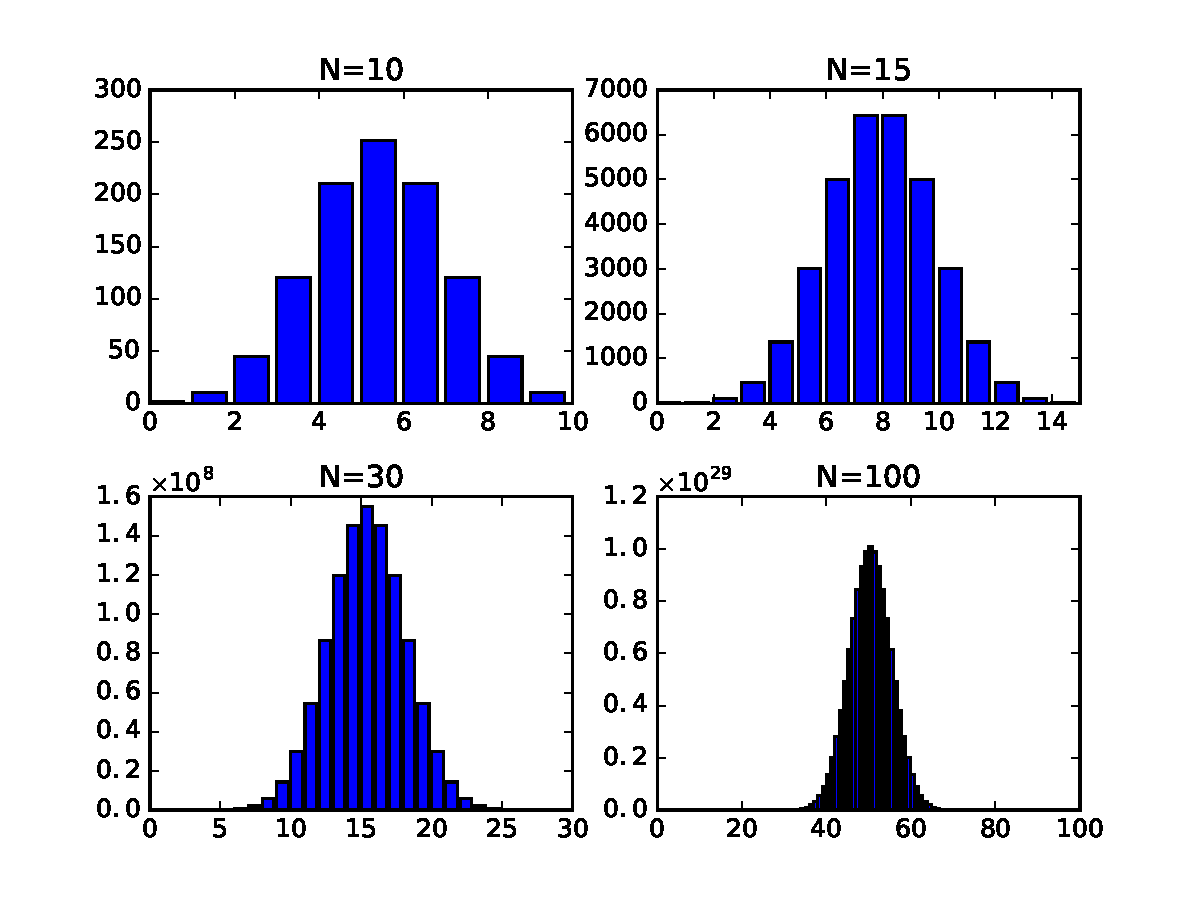
\includegraphics[width=9cm]{imgs/flip}
\caption{The value of $\Omega$ as a function of $N$ in the game of flipping coins. }
\end{figure}

\begin{figure}[h]
\centering
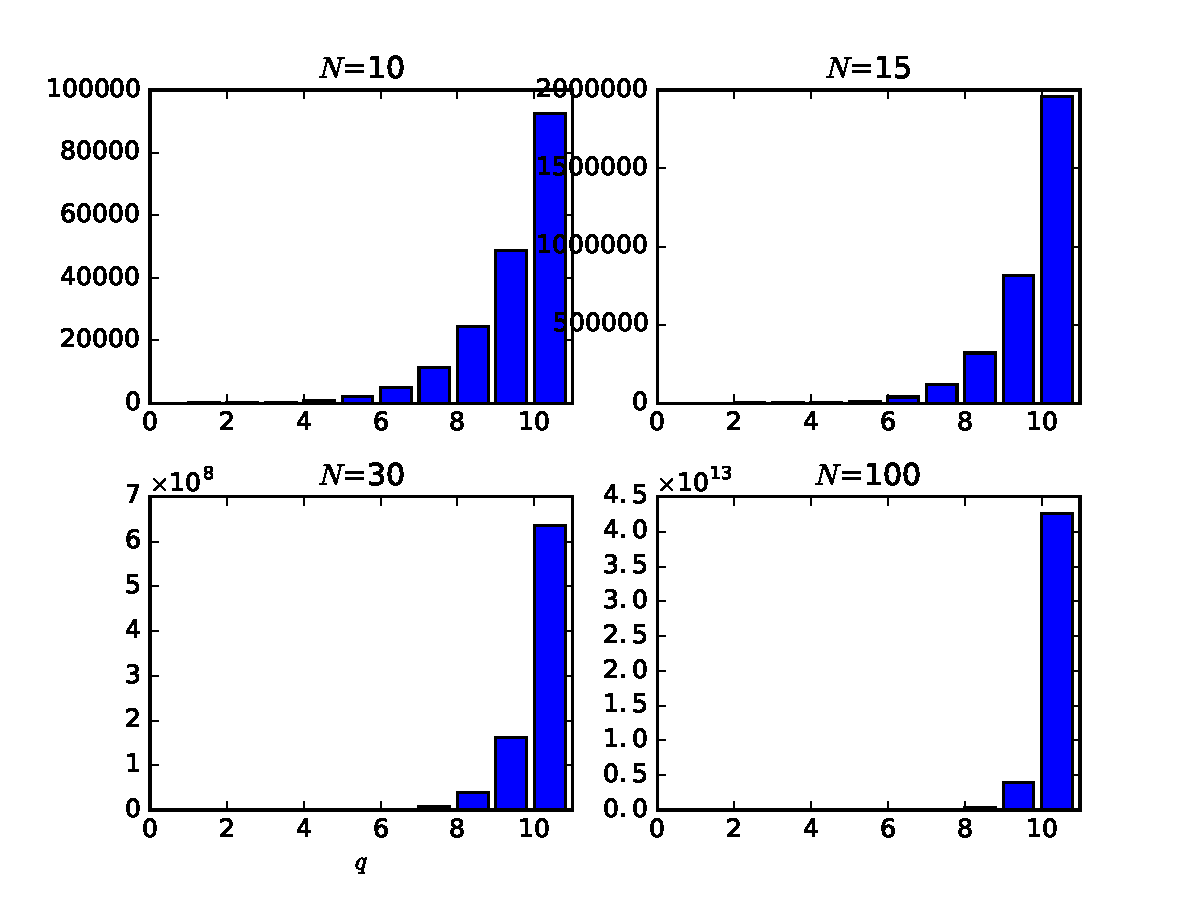
\includegraphics[width=9cm]{imgs/Einstein0}
\caption{The value of $\Omega$ as a function of $N$ in an Einstein solid. }
\end{figure}



\lecture{6}{The Second Law and Entropy}{Qiang Zhu}{scribe-name1,2,3}
%\footnotetext{These notes are partially based on those of Nigel Mansell.}
% **** YOUR NOTES GO HERE:
% Some general latex examples and examples making use of the
% macros follow.  
%**** IN GENERAL, BE BRIEF. LONG SCRIBE NOTES, NO MATTER HOW WELL WRITTEN,
%**** ARE NEVER READ BY ANYBODY.

%\section{Some useful equations} % Don't be this informal in your notes!
%\begin{equation} \label{idealgas} PV = nRT = NkT \end{equation}
%\begin{equation} \label{Avogadro} N = n \times N_A \end{equation}
%\begin{equation} \label{PV-micro} PV = Nm{\overline v_x^2} = NkT\end{equation}
%\begin{equation} \label{eqpartition} U_\text{thermal} = N \cdot f \cdot \frac{1}{2}kT %\end{equation}
%\begin{equation} \label{1stlaw} \Delta{U} = Q + W \end{equation}
%\begin{equation} \label{work3} \Delta W = - P \Delta{V} \end{equation}

\section{Two Interacting Einstein Solids}
In the previous section, we just learned how to count the $\Omega$ for an Einstein solid.
Remember we are trying to understand how heats are transferred, which essentially at least two solids.
Let's call the two solids $A$ and $B$ separately. \\\\
\begin{figure}[h]
\centering
\begin{tikzpicture}[thick]
\draw (0,0.4) -- (8,0.4) -- (8,4) -- (0,4) -- (0,0.4);
\draw (0.2,0.6) -- (3.2,0.6) -- (3.2,3.8) -- (0.2,3.8) -- (0.2,0.6);
\node at (1.8,2.8) {Solid $A$};
\node at (1.8,2.2) {$N_A$, $q_A$};
\draw (7.8,0.6) -- (4.8,0.6) -- (4.8,3.8) -- (7.8,3.8) -- (7.8,0.6);
\node at (5.8,2.8) {Solid $B$};
\node at (5.8,2.2) {$N_B$, $q_B$};
\draw [->,decorate,decoration=snake] (3.2,2) -- (4.8,2);
\draw [->,decorate,decoration=snake] (4.8,3) -- (3.2,3);
\end{tikzpicture}
\caption{Two interacting Einstein solids isolated from the rest of the universe.}
\end{figure}


Assuming that $A$ and $B$ are weakly coupled (just like what we did on ideal gas model),
the individual energies of the solids, $q_A$ and $q_B$ will change slowly.
Under this assumption, the total number of energies $q_\text {total}$ will be simple the sum of $q_A$ and $q_B$.

To make life easier, let's fix $q_\text{total}$, what's the number of multiplicity for any arbitrary $q_A$?
If we just count $A$,
\begin{equation}
 \Omega(A) = \binom{q_A+N_A-1}{q_A},
\end{equation}

In the meantime, we also needs to consider $B$, 
\begin{equation}
 \Omega(B) = \binom{q_B+N_B-1}{q_B},
 q_B = q_ \text {total} - q_A.
\end{equation}

Of course, the total number follows
\begin{equation}
 \Omega(\text {total}) = \Omega(A)\Omega(B).
\end{equation}

{\bf Exercises}\\
Write a table of $q_A$, $\Omega(A)$, $q_B$, $\Omega(B)$, $\Omega$(total), when $q_A$ + $q_B$ = 5, $N_A$=$N_B$=6.

\begin{table}[h]
\centering
\begin{tabular}{|c| c |c |c |c|}\hline
$q(A)$ & $\Omega(A)$ & $q(B)$ & $\Omega(B)$ & $\Omega$(total)\\\hline
    0  &             &        &             &  \\\hline
    1  &             &        &             &  \\\hline
    2  &             &        &             &  \\\hline
    3  &             &        &             &  \\\hline
    4  &             &        &             &  \\\hline
    5  &             &        &             &  \\\hline
\end{tabular}
\end{table}

\section{Stirling Approximation}
To apply these formulas to large systems, we need a trick for evaluating factorials of large numbers. Here is a trick called {\bf Stirling approximation},
\begin{equation}\label{stir}
  N! = N^N e^{-N} \sqrt{2\pi N}
\end{equation}

This can be roughly understood that $N$! is firstly approximated as $N^N$, then averaged by $(N/e)^N$, 
\begin{equation}
  N! = N^N e^{-N} 
\end{equation}

A more elegant way to express $N$! is to use the so called \textbf{Gamma function}. Suppose you start with the integral,
\begin{equation} \int ^\infty _0 e^{-ax} dx = 1/a \end{equation}
and repeat doing differentiation with respect to $a$, you will eventually get
\begin{equation} \int ^\infty _0 x^n e^{-ax} dx = n! a^{-(n+1)} \end{equation}
Starting with this equation, you are able to prove eq \ref{stir}.
From the above, you can get the logarithm as follows
\begin{equation}\label{s1}
      \ln N!  = N \ln N - N - 1/2 \ln (2\pi N) 
\end{equation}

When N is very large, we can safely remove the last term,
\begin{equation}\label{s2}
  \text {ln}N! = N \text {ln}N - N ~~~~~~~~ (\text {when} ~N\rightarrow \infty )
\end{equation}

Alternatively, you can solve it in this way,
\begin{equation}\label{s1}
\begin{split}
      \ln N! & = \ln N + \ln (N-1) + \ln (N-2) + ...    \\
             & \approx \int_0^N \ln x dx \\
             & = N \ln N - N - 1/2 \ln (2\pi N) \\
\end{split}
\end{equation}





\section{Computer Programming}
\begin{enumerate}
\item Write a code to calculate $\Omega$ as a function of $q_A$, when $N_A$=[300, 600, 3000, 6000], $N_B$=[200, 400, 2000, 4000],
and $q$=100, plot them and try to find some tendency when $N$ increases (hint: 4 plots).
\begin{figure}[h]
\centering
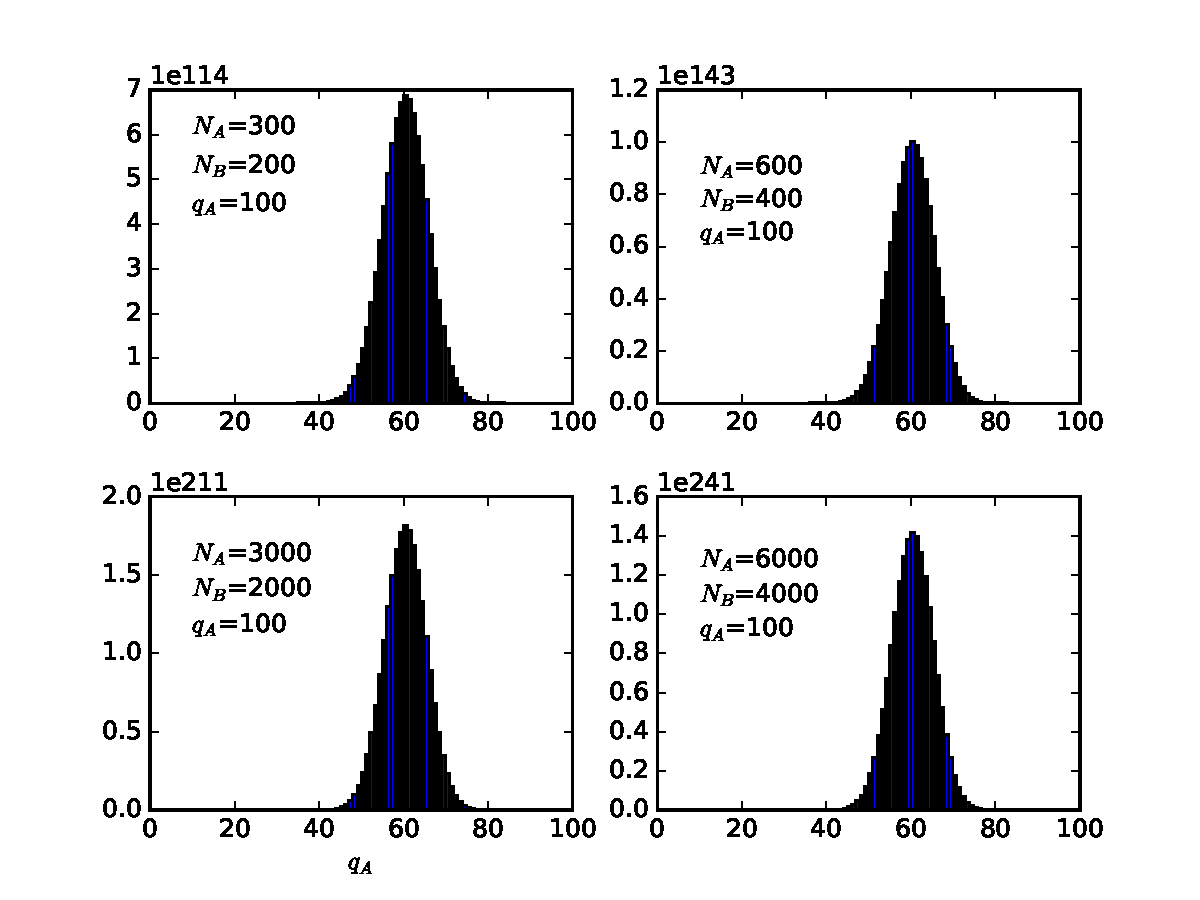
\includegraphics[width=12cm]{imgs/Einstein.pdf}
\caption{$\Omega$ as a function of $N$ in two interacting Einstein solids. }
\end{figure}
\item Write a code to calculate the probability of $\Omega(q_A)$, when $N_A$=[300, 3000], $N_B$=[200, 2000],
for $q$=[100, 1000], plot them and try to explain the differences. (hint: 2 plots)

\begin{figure}[h]
\centering
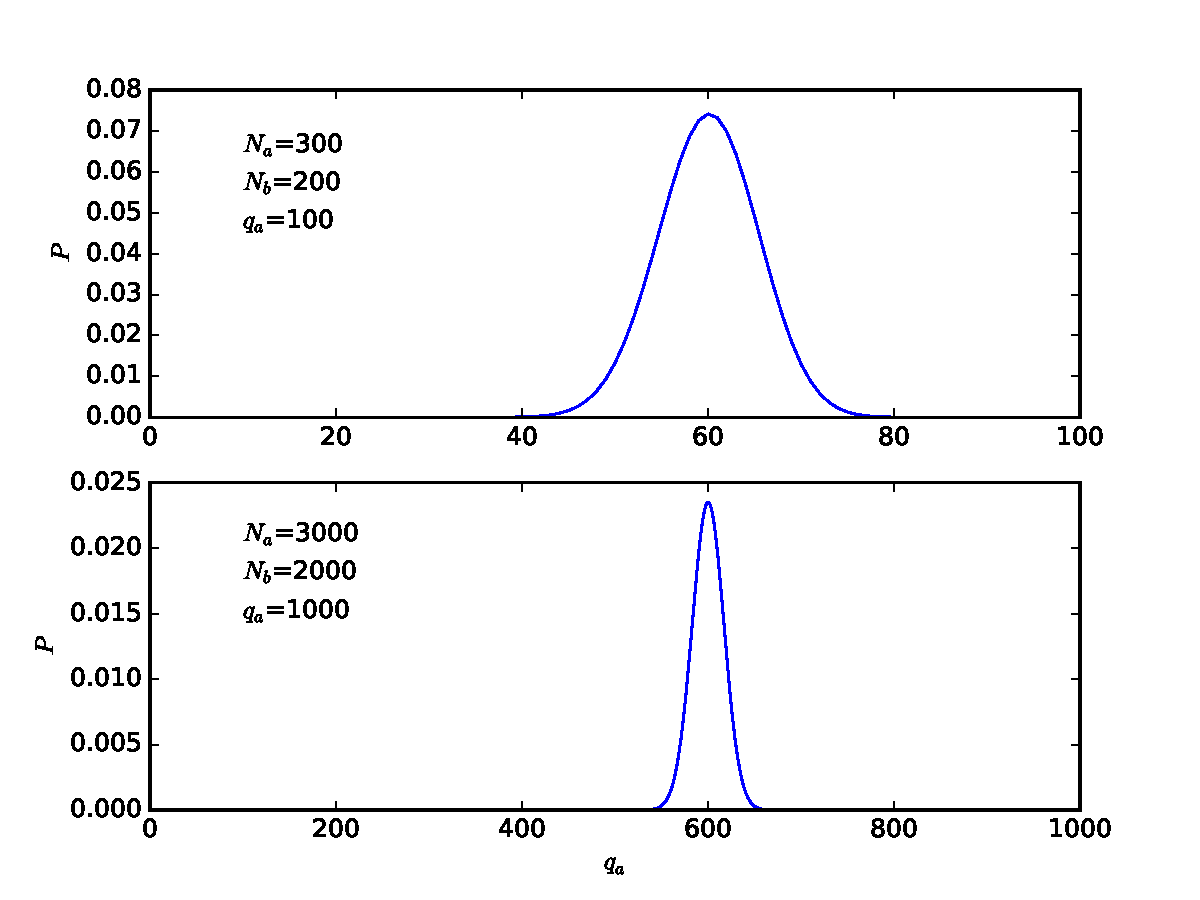
\includegraphics[width=10cm]{imgs/Einstein2.pdf}
\caption{Probability distribution of $\Omega(N)$ in two interacting Einstein solids for different $q$ values. }
\end{figure}

\item Write a code to show the comparison of Stirling approximation in eq.\ref{s1} and \ref{s2}
\begin{figure}[h]
\centering
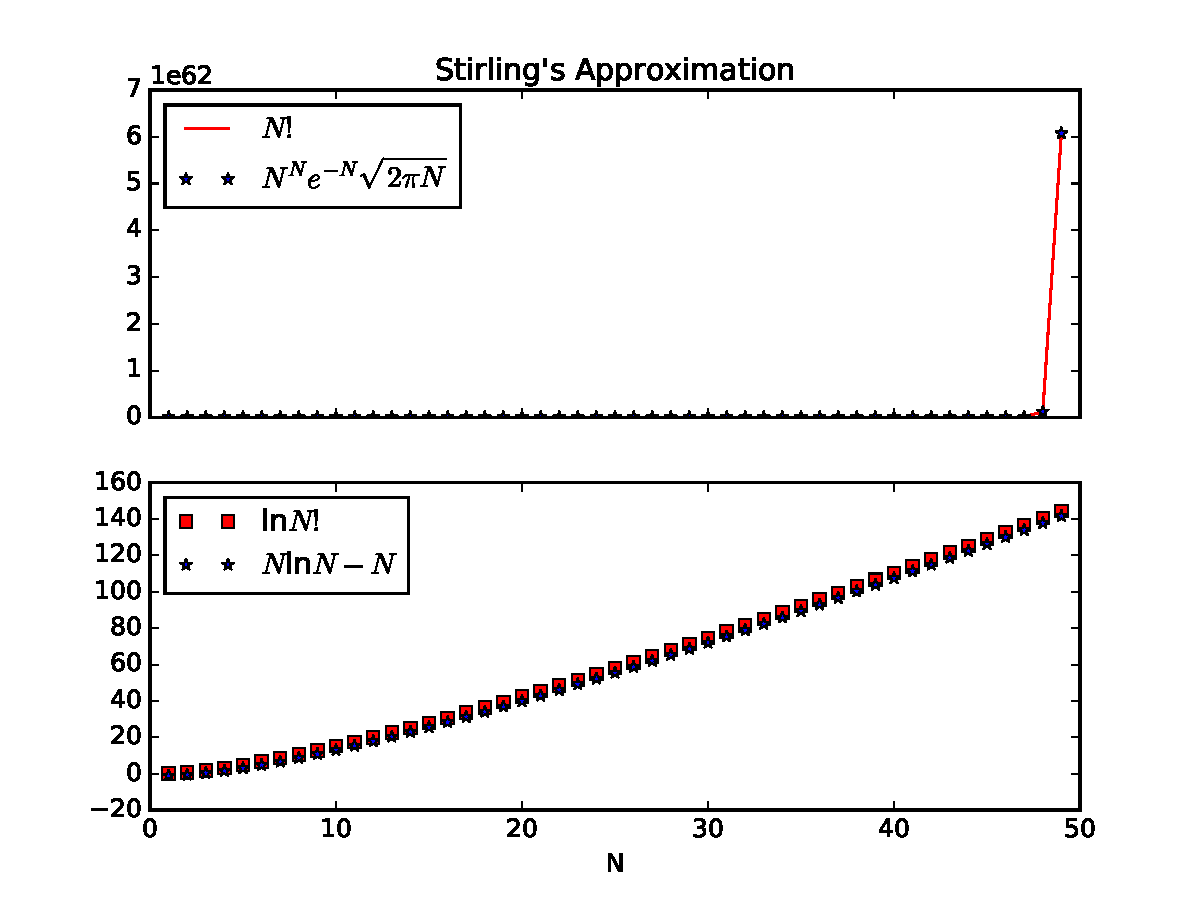
\includegraphics[width=8cm]{imgs/Stirling.pdf}
\caption{The accuracy of Stirling approximation. }
\end{figure}

\item The Gamma function is defined as 
\begin{equation} \Gamma(n+1) = \int ^\infty _0 x^n e^{-x} dx, \end{equation}
write a code to show the comparison of $\Gamma(n+1)$, $n$!, and $\sqrt{2\pi n}(n/e)^n$ in the range of [0,3.6]
\begin{figure}[h]
\centering
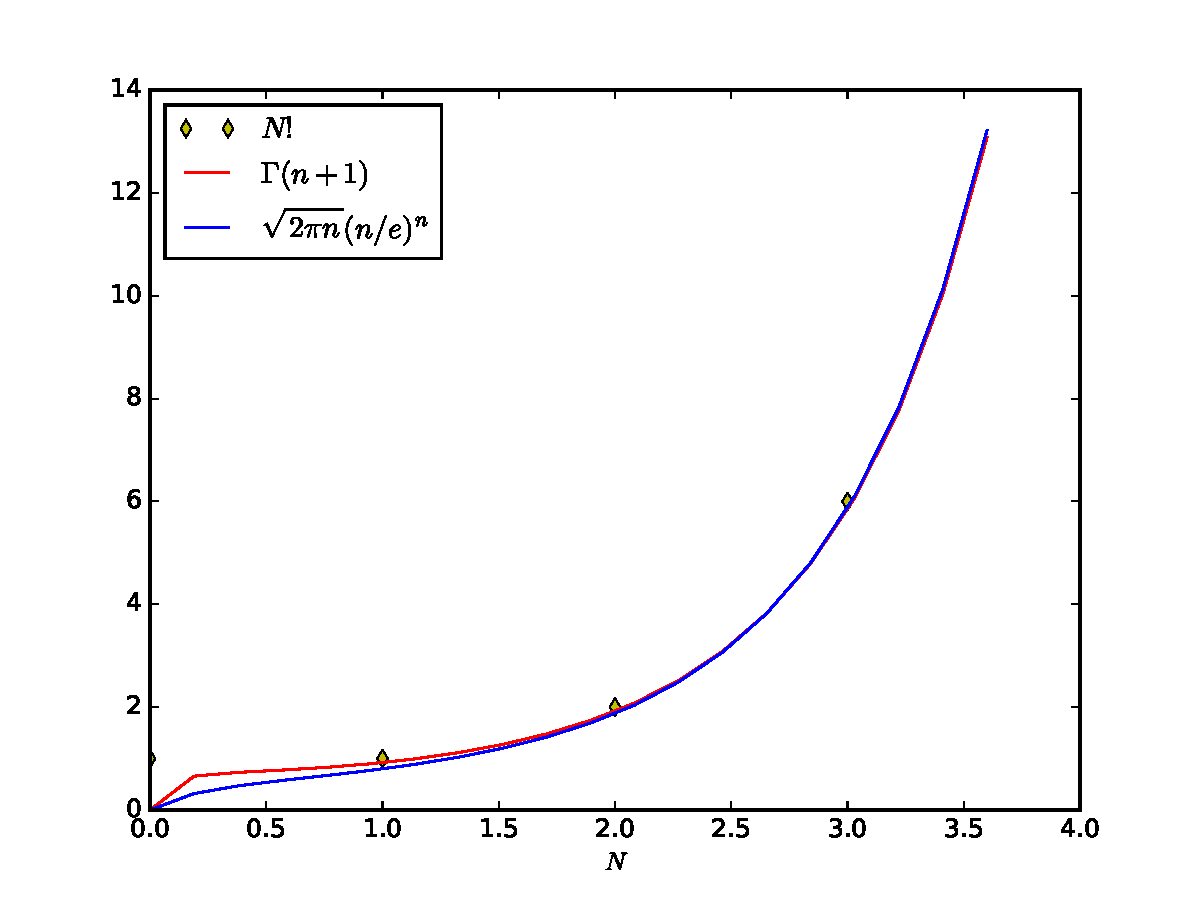
\includegraphics[width=6cm]{imgs/Stirling2.pdf}
\caption{Comparison between the Gamma function and Stirling approximation. }
\end{figure}


\end{enumerate}

\lecture{7}{The Second Law and Entropy}{Qiang Zhu}{scribe-name1,2,3}


\section{Calculate $\Omega$ for a Einstein Solid}
Remember we have done some computer programmings for two-state systems.
A general trend is that it approaches to a large number $N$, $\Omega(N)$ tends to be localized.
If we treat the histogram of $\Omega(N)$ as a continues function (true when $N$ is very large),
it looks like a very smooth curve and $\Omega(N)$ follows some kind of distribution. 

Now let's try to figure out what it is, by taking a Einstein solid as an example. 
\begin{equation} \label{E0}
 \Omega(N, q) = \binom{q+N-1}{q} = \frac{(q+N-1)!}{q!(N-1)!}
\end{equation}

In reality, there are always many more energy units ($q$) than oscillator ($N$), so we assume $q\gg N$.

To make it easier, let's just remove \textit{-1} in eq. \ref{E0},
\begin{equation} \label{E1}
\begin{split}
 \text{ln}\Omega &= \text{ln}(\frac{(q+N)!}{q!N!})\\
         &= \text{ln}(q+N)! - \text{ln}q! - \text{ln}N!\\
   &\approx (q+N)\text{ln}(q+N) - (q+N) - q\text{ln}q - q - N\text{ln}N - N\\
        & = (q+N)\text{ln}(q+N) - q\text{ln}q - N\text{ln}N \\
\end{split}
\end{equation}

Remember we have the assumption of $q\gg N$, namely ($q/N \rightarrow$ 0)
\begin{equation} \label{E2}
       \text{ln}(q+N) = \text{ln}(q(1+\frac{N}{q}))\\
                      = \text{ln}q + \frac{N}{q} 
\end{equation}

Therefore, we have 
\begin{equation} \label{E3}
       \text{ln}\Omega = N\text{ln}\frac{q}{N} + N + \frac{N^2}{q}\\
                 \approx N\text{ln}\frac{q}{N} + N 
\end{equation}

If we remove the logarithm sign,
\begin{equation} \label{E4}
       \Omega(N,q) = (\frac{eq}{N})^N
\end{equation}


\section{Calculate $\Omega$ for two Einstein Solids}
Naturally, we now know the general form of two Einstein Solids model,
\begin{equation} \label{E5}
       \Omega(N_A,q_A,N_B,q_B) = (\frac{eq_A}{N_A})^{N_A} (\frac{eq_B}{N_B})^{N_B}
\end{equation}

For simplicity, let make $N_A = N_B = N $, then
\begin{equation} \label{E6}
       \Omega(N,q_A,q_B) = (\frac{e}{N})^{2N} (q_A q_B)^{N}
\end{equation}

Based on what we plot in the homework, we know that $\Omega$ reaches its maximum value at 
$q_A = q_B = q$/2,
\begin{equation}
       \Omega_\text{max} = (\frac{e}{N})^{2N} (q/2)^{2N}
\end{equation}

Now let's try to calculate the points near $q$/2, say,
\begin{equation}
  q_A = q/2+x, ~~~~~~~~~ q_B=q/2-x.
\end{equation}

Using eq. \ref{E6},
\begin{equation} \label{E7}
       \Omega(N,q,x) = (\frac{e}{N})^{2N} ((\frac{q}{2})^2-x^2)^{N}.
\end{equation}

To simplify it, we get
\begin{equation} \label{E8}
\begin{split}
       \text{ln}((\frac{q}{2})^2-x^2)^{N} 
           &= N[\text{ln}[(\frac{q}{2})^2-x^2]\\
           &= N[\text{ln}(\frac{q}{2})^2 + \text{ln}(1-(\frac{2x}{q})^2))]\\
           &= N[\text{ln}(\frac{q}{2})^2 - (\frac{2x}{q})^2)]\\
           &= N[\text{ln}(\frac{q}{2})^2 - (\frac{2x}{q})^2)]
\end{split}                                          
\end{equation}
hence we have 
\begin{equation} \label{E9}
  \Omega = \Omega_\text{max} \cdot e^{-N(2x/q)^2}
\end{equation}
This is a typical Gaussian function. A standard version is as follows,
\begin{equation}
  f(x|\mu,\delta^2) = \frac{1}{\sqrt{2\delta^2}\pi} e^\frac{-(x-\mu)^2}{2\delta^2}.
\end{equation}

\begin{tikzpicture}[x=1.5cm, y=1.5cm]

%normal distribution function 'normaltwo'
    \def\normaltwo{\x,{4*1/exp(((\x-3)^2)/2)}}
% input y parameter
    \def\y{3.5}
% this line calculates f(y)
    \def\fy{4*1/exp(((\y-3)^2)/2)}
% Shade orange area underneath curve.
    %\fill [fill=orange!60] (2.6,0) -- plot[domain=0:4.4] (\normaltwo) -- ({\y},0) -- cycle;
% Draw and label normal distribution function
    \draw[color=blue,domain=0:6] plot (\normaltwo) node[right] {};
% Add dashed line dropping down from normal.
    \draw[dashed] ({\y},{\fy}) -- ({\y},0)     node[below] {$\mu+\delta$};
    \draw[dashed] ({6-\y},{\fy}) -- ({6-\y},0) node[below] {$\mu-\delta$};
% Optional: Add axis labels
    \draw (-.2,2.5) node[left] {$f(x)$};
    \draw (3,-.5) node[below] {$x$};
% Optional: Add axes
    \draw[->] (0,0) -- (6.2,0) node[right] {};
    \draw[->] (0,0) -- (0,5) node[above] {};
\end{tikzpicture}
\begin{enumerate}
\item symmetric
%\item unimodal
%\item its second derivetive is equal to 
\item Gaussian width
\end{enumerate}



The multiplicity falls off to 1/e of its maximum when 
\begin{equation}
  N(\frac{2x}{q})^2 = 1 ~~~~~~or~~~~~~ x = \frac{q}{2\sqrt{N}}
\end{equation}

Let's plug in some number, say $N$=\textrm {$10^{20}$}, 
This results tell us,
when two Einstein solids are in thermodynamical equilibrium, any random fluctuation
will be not measurable. The most-likely macrostates are very localized.\\
{\bf Exercises}
\begin{enumerate}
\item Problem 2.20. 
\item Problem 2.23
\end{enumerate}

\section{Ideal Gas}
Suppose we have a single gas atom (Ar), with kinetic energy $U$ in a container of volume $V$, what is its corresponding $\Omega$?
Obviously, the possible microstate is proportional to V. In principle, the atom can stay at any place of $V$.
Also, each microstate can be represented as a vector, since it has velocity (more precisely Momentum). 
Therefore
\begin{equation}
\Omega \approx V\cdot V_p
\end{equation}



It appears that both $V$ and $V_p$ somehow relate to very large numbers, would their product go to infinity? 
Fortunately, we have the famous {\bf Heisenberg uncertainty principle}:
\begin{equation} \Delta{x}\Delta{p_x} = h. \end{equation}

For a one-dimensional chain, we define $L$ as the length in real space, $L_p$ as the length in momentum space,
\begin{equation} \Omega_{1D} = \frac{L}{\Delta{x}} \frac{L_p}{\Delta{p_x}} = \frac{LL_p}{h}. \end{equation}
Therefore, its 3D version is,
\begin{equation} \Omega_1 = \frac{VV_p}{h^3}. \end{equation}
Accordingly, the multiplicity function for an ideal gas of two molecules should be
\begin{equation} 
\Omega_2 = \frac{1}{2}\frac{V^2}{h^6} \times \text{area of $P$ hypersphere}
\end{equation}
if the two molecules are indistinguishable.
The general form for $N$ should be 
\begin{equation} \Omega_N = \frac{1}{N!}\frac{V^N}{h^{3N}} \times \text{area of $P$ hypersphere}. \end{equation}

For $N$=1, how to calculate the area?
Since $U$ depends on the momentum by
\begin{equation}
U = \frac{1}{2}m(v_x^2+v_y^2+v_z^2)=\frac{1}{2m}(p_x^2+p_y^2+p_z^2)
\end{equation}
\begin{equation}
p_x^2+p_y^2+p_z^2 = \sqrt{2mU}
\end{equation}

So the momentum space is the surface of a sphere with radius $\sqrt{2mU}$, namely,
\begin{equation}
\begin{split}
\text{area} = & 2    ~~~~~~~~~~~~~~~~~~~~~~~~\text {($d$=1)}\\
            = & 2\pi r    ~~~~~~~~~~~~~~~~~~~\text {($d$=2)}\\
            = & 4\pi r^2    ~~~~~~~~~~~~~~~~~\text {($d$=3)}\\
            = & ....\\
            = & ....\\
            = & \frac{2\pi^{d/2}}{\Gamma(d/2)} r^{d-1} ~~~~~\text {($d$ in general)}\\
\end{split}
\end{equation}

Therefore, the general $\Omega$ is
\begin{equation} 
\Omega_N = \frac{1}{N!} \frac{V^N}{h^{3N}} \frac{2\pi^{3N/2}}{(3N/2-1)!} \sqrt{2mU}^{3N-1}. 
\end{equation}


\begin{equation}
\Omega(U,V,N) = f(N)V^NU^{3N/2}
\end{equation}
where $f(N)$ is a complicated function of $N$.\\

For two interaction gases,
\begin{equation}
\Omega(U,V,N) = [f(N)]^2(V_AV_B)^N(U_AU_B)^{3N/2}
\end{equation}


%\appendix
\section{Appendix: Area of high-dimensional Hypersphere}
For a d-dimensional hypersphere with a radius of $r$, we can solve it iteratively.
When $d$=1, $A(r)$=2, $d$=2, $A(r)=2\pi r$
\begin{equation}
    A_3(r) = \int_0^{\pi} A_2(r\sin\theta)rd\theta = 2\pi r^2 \int_0^{\theta}d\theta = 4\pi r^2.
\end{equation}
Consequently, we can keep doing this
\begin{equation}
\begin{split}
    A_d(r) = & \int_0^\pi{A_{d-1}(r\sin(\theta))rd\theta} \\
           = & \int_0^\pi\frac{2\pi^{(d-1)/2}}{\Gamma(\frac{d-1}{2})}(r\sin\theta)^{d-2}rd\theta \\
           = & \frac{2\pi^{(d-1)/2}}{\Gamma(\frac{d-1}{2})}r^{d-1} \int_0^{\pi}(\sin\theta)^{d-2}d\theta\\
\end{split}
\end{equation}

\begin{equation}
    \int_0^{\pi} (\sin\theta)^nd\theta = \frac{\sqrt{\pi}\Gamma(\frac{n+2}{2})}{\Gamma(\frac{n+2}{2})}
\end{equation}

so
\begin{equation}
    A_d(r) = \frac{2\pi^{d/2}}{\Gamma(d/2)}r^{d-1}
\end{equation}



\lecture{8}{The Second Law and Entropy}{Qiang Zhu}{scribe-name1,2,3}


\section{Entropy}
\begin{equation} \label{entropy} 
S = k \text{ln}\Omega 
\end{equation}

\section{Entropy of Einstein Solid}
\begin{equation} \label{entropy} 
S = k\text{ln}(eq/N)^N = Nk[\text{ln}(q/N)+1]
\end{equation}
if $N$=\textrm{$10^{22}$}, $q$=\textrm{$10^{24}$}
\begin{equation} \label{entropy} 
S = Nk(~~~~~~~~~~~~~~~~~)= ~~~~~~~~~~~~~\text{J/K} 
\end{equation}

\begin{enumerate}
\item Discuss the relation between $S$ and $q$, $N$?
\item Mixing A and B?
\item Entropy tends to increase?
\end{enumerate}

{\bf Exercise} \\
Based on Figure 2.5, compute the entropy of the total, most likely, least likely macrostate. Compare them with the number of typical values (0.77J/K).

\section{Entropy of an Ideal Gas}
\begin{equation} \label{entropy} 
S = Nk[\text{ln}(\frac{V}{N} (\frac{4\pi m U}{3Nh^2})^{3/2}) + \frac{5}{2}]
\end{equation}

This is called \textbf{Sackur-Tetrode equation}.

\begin{enumerate}
\item Discuss the relation between $S$ and $V$, $N$, $m$, $U$, compare it with Einestein solid?
\item Compute $S$ for He/Ar? (Same $N$, $V$, $U$, the radius hypersurface of $P$ is $\sqrt{2mU}$ ) 
\item Free expansion? How to calculate $\Delta{S}$, with alternative way?
\end{enumerate}

\begin{figure}[h]
\centering
\begin{tikzpicture}[thick]
\draw (8,4) -- (0,4) -- (0,0.4) -- (8,0.4);
\draw (8,3.8) -- (0.2,3.8) -- (0.2,0.6) -- (8,0.6);
\draw [line width=0.2cm](4,3.8) -- (4,0.6); 
\draw [->](4,2) -- (4.8,2) node[right]{piston}; 
\node at (1.8,2.8) {gas};
\node at (3.6,4.4) {(a) isothermal expansion};

\draw (10,0.4) -- (18,0.4) -- (18,4) -- (10,4) -- (10,0.4);
\draw (10.2,0.6) -- (14.0,0.6) -- (14.0,3.8) -- (10.2,3.8) -- (10.2,0.6);
\node at (11.8,2.8) {gas};
\draw (17.8,0.6) -- (14.0,0.6) -- (14.0,3.8) -- (17.8,3.8) -- (17.8,0.6);
\node at (15.8,2.8) {vacuum};
\node at (13.6,4.4) {(b) free expansion};
\draw [->] (14,2) -- (14.8,2.4);
\draw [->] (14,2) -- (14.8,1.6);
\draw (14,2) circle (0.2cm);
\end{tikzpicture}
\end{figure}


\section{Mixing Entropy of an Ideal Gas}
If we mix two different gases, A and B, each with the same $U$, $V$ and $N$, they occupy two halves of a divided chamber.
\begin{equation}\Delta S_A = Nk\text{ln} V_f/V_i = Nkln2 \end{equation}
\begin{equation}\Delta S_B = Nk\text{ln} V_f/V_i = Nkln2 \end{equation}
\begin{equation}\Delta S_\text{total} = 2Nkln2 \end{equation}

What if $A$ and $B$ are indistinguishable? (double counting?)
Mixing only applies when $A$ and $B$ are different?
\begin{figure}[h]
\centering
\begin{tikzpicture}[thick]
\draw (8,4) -- (0,4) -- (0,0.4) -- (8,0.4) -- (8,4);
\draw (7.8,3.8) -- (0.2,3.8) -- (0.2,0.6) -- (7.8,0.6) -- (7.8,3.8);
\draw [line width=0.2cm](4,3.8) -- (4,0.6); 
\draw [->](4,2) -- (4.8,2) node[right]{piston}; 
\node at (1.8,2.8) {1 mol He gas};
\node at (5.8,2.8) {1 mol Ar gas};
\node at (3.6,4.4) {(a) remove the piston};


\draw (10,0.4) -- (18,0.4) -- (18,4) -- (10,4) -- (10,0.4);
\draw (10.2,0.6) -- (17.8,0.6) -- (17.8,3.8) -- (10.2,3.8) -- (10.2,0.6);
\node at (13.8,1.8) {1 mol He(g)};
\draw [-> ](14,4.0) -- (14,2.6);
\node at (13.6,4.4) {(b) add 1 mol He/Ar(g)};
\draw (14,3.9) circle (0.2cm);
\end{tikzpicture}
\end{figure}


\section{Irreversible process}
\begin{enumerate}
\item Entropy increase $\rightarrow$ irreversible
\item Entropy unchanged $\rightarrow$ reversible
\item Slow compression, quasi static, reversible
\item Heat flow is always irreversible
\item Mixing (+$V$), stir salt in to soup, scrambling egg
\item +$N$, Burning gasoline, large molecule to small molecules, Cut down a tree
\end{enumerate}

\ce{CH4(gas) + 2O2(gas) -> CO2(gas) + 2H2O(gas)} ~~~~~~~S\\
\ce{2H2(gas) + O2(gas) -> 2H2O(gas)}~~~~~~~~~~~ S\\
If you consider it is not a isolated system. It also produce heat, so the total entropy is increasing due to heat.

\section{Homework}
Prove that 1 mol Ar gas has larger entropy than 1 mol He.\\
Problems 2.17, 2.18, 2.22, 2.29, 2.30, 2.31, 2.32, 2.34, 2.37



\lecture{9}{Entropy and Heat}{Qiang Zhu}{scribe-name1,2,3}
%\footnotetext{These notes are partially based on those of Nigel Mansell.}
% **** YOUR NOTES GO HERE:
% Some general latex examples and examples making use of the
% macros follow.  
%**** IN GENERAL, BE BRIEF. LONG SCRIBE NOTES, NO MATTER HOW WELL WRITTEN,
%**** ARE NEVER READ BY ANYBODY.

\section{Express Temperature with respect to Entropy}
Show that during the quasi-static isothermal expansion, the change of entropy is related to the heat input $Q$ by
\begin{equation} \label{entropy} 
\Delta{S}=\frac{Q}{T}     ~~~~~~~~ \rightarrow~~~~~~~~  T = \frac{Q}{\Delta{S}}
\end{equation}

It looks like $T$ can expressed as energy divided by entropy.

\begin{figure}[h]
\centering
{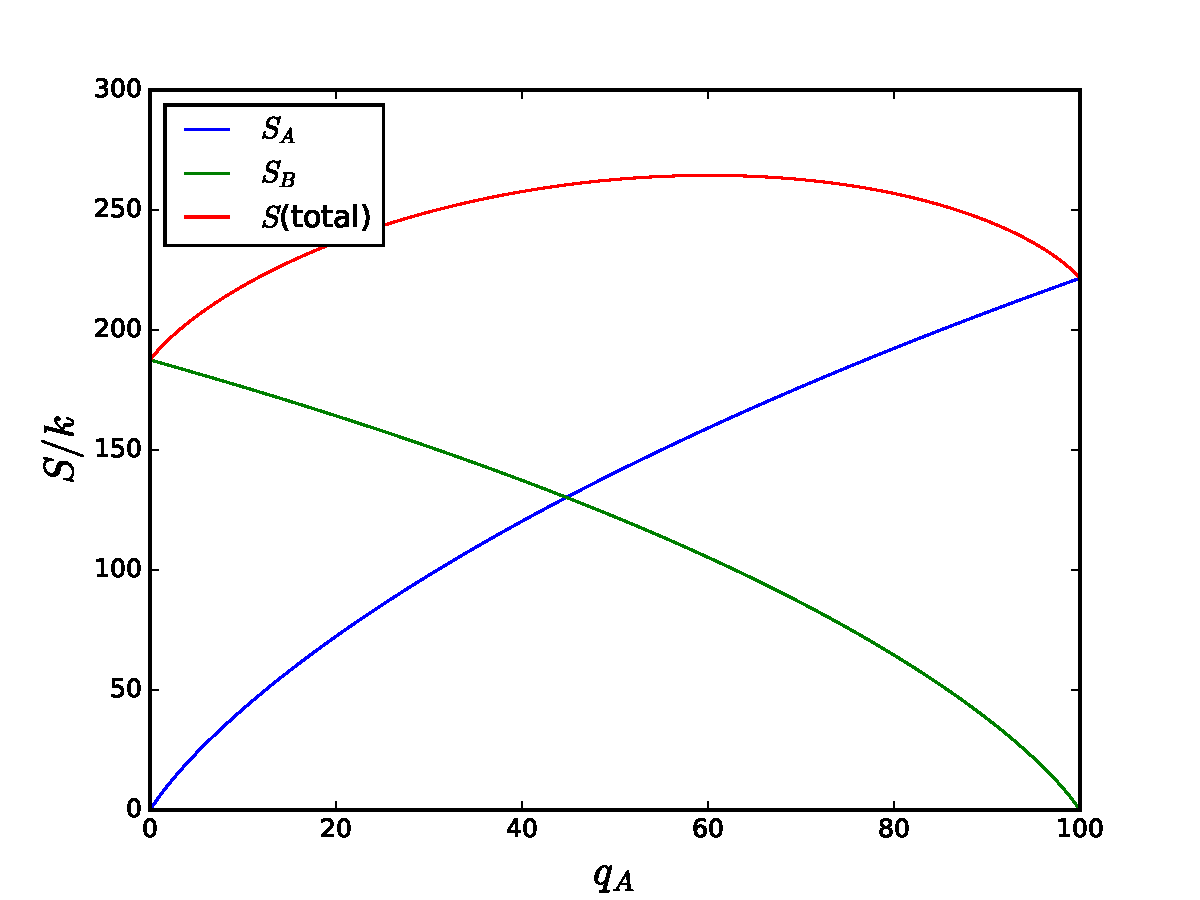
\includegraphics[width=12cm]{imgs/Einstein3}}
\caption{\label{dS} Entropy as a function of $q_A$ in two interacting Einstein solids ($N_A$=300, $N_B$=200, $q$(total)=100). }
\end{figure}


In the context of two interacting Einstein solid, we once calculated $\Omega$ as a function of $q_A$. Let's redo it.
At equilibrium, we know $S_\text{total}$ reaches the maximum, therefore,
\begin{equation} \label{entropy} 
\frac {\partial{S_\text{total}}} {\partial{q_A}}=0     ~~~~~~~~ \rightarrow~~~~~~~~  \frac {\partial{S_\text{total}}} {\partial{U_A}}=0
\end{equation}

Since $S_\text{total}$ is simply the sum of $S_A$ and $S_B$, we now know
\begin{equation} \label{entropy} 
\frac {\partial{S_A}} {\partial{U_A}} +  \frac {\partial{S_B}} {\partial{U_A}} =0     ~~~~~~~~ \rightarrow~~~~~~~~  
\frac {\partial{S_A}} {\partial{U_A}} =  \frac {\partial{S_B}} {\partial{U_B}} 
\end{equation}

At equilibrium, which quantity of $A$ and $B$ becomes equivalent? \\
The consequence of heat flow?\\
Check the unit! Yes, the slope of $S_A$ is actually the reciprocal of $T$.\\
Therefore we have
\begin{equation} 
1/T = \Bigg(\frac {\partial{S}} {\partial{U}}\Bigg)_{N, V} ~~~~~~~~ \rightarrow~~~~~~~~ T = \Bigg(\frac {\partial{U}} {\partial{S}}\Bigg)_{N, V}.
\end{equation}

{\bf Exercise}\\
Calculate the slope of $S$-$q$ graph for various points. (assuming $\epsilon$=0.1eV, 0.024 eV is about 300 K, )\\
\begin{enumerate}
\item $q$=0,  $(\frac {\Delta{S_A}} {\Delta{U_A}})^{-1}$=  ~~~~~~~~~~~~~~~~~~~~~~~~~~~~~~  $(\frac {\Delta{S_B}} {\Delta{U_B}})^{-1}$= 
\item $q$=10, $(\frac {\Delta{S_A}} {\Delta{U_A}})^{-1}$=  ~~~~~~~~~~~~~~~~~~~~~~~~~~~~~~  $(\frac {\Delta{S_B}} {\Delta{U_B}})^{-1}$= 
\item $q$=60, $(\frac {\Delta{S_A}} {\Delta{U_A}})^{-1}$=  ~~~~~~~~~~~~~~~~~~~~~~~~~~~~~~  $(\frac {\Delta{S_B}} {\Delta{U_B}})^{-1}$= 
\end{enumerate}

\section{Einstein Solid}

\begin{equation} S = Nk[\text{ln}(q/N)+1] = Nk\text{ln}U - Nk\text{ln}(\epsilon N) + Nk \end{equation}
\begin{equation} T = (\frac {\partial{S}} {\partial{U}})^{-1} = (\frac{Nk}{U})^{-1}\end{equation}
\begin{equation} U = NkT \end{equation}
This is exactly the thermal equipartition theorem applied to an Einstein Solid.

\section{Ideal Gas}

\begin{equation} S = Nk\text{ln}V + 3/2Nk\text{ln}U - Nk\text{ln}(f(N)) \end{equation}
\begin{equation} T = (\frac {\partial{S}} {\partial{U}}) ^{-1} = ~~~~~\end{equation}
\begin{equation} U = 3/2NkT \end{equation}


\section{Measuring Entropy}
\begin{equation} dS = \frac{dU}{T} = \frac{Q}{T}   ~~~~~~~~~~~~~~~~~ \text{(constant volume, W = 0)}\end{equation}
\begin{equation} dS = \frac{C_VdT}{T}   ~~~~~~~~~~~~~~~~~ \text{(constant volume, W = 0)}\end{equation}
\begin{equation} \Delta{S} = S_f-S_i = \int^{T_f}_{T_i} \frac{C_V}{T} dT \end{equation}
\begin{equation} \Delta{S} = \int^B_A \frac{C_V}{T} dT \end{equation}

What is $S$ when $T$=0, in principle $\Omega$=1, so $S$=0.\\
However, solid crystals have residual entropy due to the random orientations, so the configuration at 0K is not 1!
For instance, each CO molecule has two possible orientations: CO or OC. Assuming they are completely random, what's the residual entropy of 1 mole CO?\\\\
$S(0K)$ = $k$ln($\Omega$) = $k$ln$2^N$ = $Nk$ln2 = ~~~~~~~~~~~~~~~~~~~~~~~~~~~~~~~~ = 5.8 J/K\\
$S(300K)$ = $S(0K) + C_V \int^{300}_{0} \frac{1}{T} dT$ = 5.8 + 2.5*8.31*ln(300) = 5.8 + 118.50 = 124.30 J/K\\\\
This value looks much smaller than the reference value in the appendix (197.67 J/K), because a constant volume assumption is not realistic.

\section{Macroscopic view}
\begin{figure}[h]
\centering
\begin{tikzpicture}[thick]
\draw (0,0.4) -- (8,0.4) -- (8,4) -- (0,4) -- (0,0.4);
\draw (0.2,0.6) -- (3.2,0.6) -- (3.2,3.8) -- (0.2,3.8) -- (0.2,0.6);
\node at (1.8,2.8) {Solid $A$};
\node at (1.8,2.2) {500 K};
\draw (7.8,0.6) -- (4.8,0.6) -- (4.8,3.8) -- (7.8,3.8) -- (7.8,0.6);
\node at (5.8,2.8) {Solid $B$};
\node at (5.8,2.2) {300 K};
\draw [->,decorate,decoration=snake] (3.2,2) -- (4.8,2) node [above, xshift=-1cm]{1500 J};
\end{tikzpicture}
\caption{A schematic heat flow between two interacting Einstein solids.}
\end{figure}
\begin{enumerate}
\item Object $A$ loses entropy by $dQ/T$ = -3 J/K 
\item Object $B$ gain  entropy by $dQ/T$ = +5 J/K 
\item The total entropy increases by +2 J/K
\item Fundamentally, the net increase in entropy is the driving force behind the flow of heat.
\item The manifestation of 2nd law
\end{enumerate}

%\section{Homework}
%Problem 3.5, 3.8, 3.11, 3.14, 3.16




\lecture{10}{Entropy and Pressure}{Qiang Zhu}{scribe-name1,2,3}


\section{Mechanical Equilibrium and Pressure}
In the last lecture, we just learned the relation between $S$ and $T$, is there any analogy between $S$ and $P$?

\begin{figure}[h]
\centering
\begin{tikzpicture}[thick]
\draw (0,0.4) -- (8,0.4) -- (8,4) -- (0,4) -- (0,0.4);
\draw (0.2,0.6) -- (4.4,0.6) -- (4.4,3.8) -- (0.2,3.8) -- (0.2,0.6);
\node at (1.8,2.8) {$U_A, V_A, S_A$};
\node at (1.8,2.2) {$P_A$};
\draw (7.8,0.6) -- (4.6,0.6) -- (4.6,3.8) -- (7.8,3.8) -- (7.8,0.6);
\node at (6.0,2.8) {$U_B, V_B, S_B$};
\node at (6.0,2.2) {$P_B$};
\draw [->,decorate,decoration=snake] (3.6,2) -- (5.0,2) node [above, xshift=-0.8cm]{pressure flow};
\end{tikzpicture}
\caption{A schematic pressure flow between two gases.}
\end{figure}

Again, we start from the condition when the system reaches its equilibrium,
\begin{equation} \label{entropy} 
\frac {\partial{S_\text{total}}} {\partial{U_A}}=0     ~~~~~~~~ \rightarrow~~~~~~~~  \frac {\partial{S_\text{total}}} {\partial{V_A}}=0
\end{equation}
as $S$ is a function of $U$ and $V$.

We already applied the 1st condition in the previous lecture. How about the 2nd condition? 
\begin{equation} \label{entropy} 
\frac {\partial{S_A}} {\partial{V_A}} +  \frac {\partial{V_B}} {\partial{V_A}} =0     ~~~~~~~~ \rightarrow~~~~~~~~  
\frac {\partial{S_A}} {\partial{V_A}} =  \frac {\partial{V_B}} {\partial{V_B}} 
\end{equation}

What's the physical meaning of $\partial{S_A}/\partial{V_A}$? \\
If we dig a bit on the units, we will find $\partial{S_A}/\partial{V_A}$ has a unit of N$\cdot$m/K, about $P/T$ hence we guess
\begin{equation} \label{entropy} 
\frac {P}{T} =  (\frac {\partial{S}} {\partial{V}})_{U,N}     ~~~~~~~~ \rightarrow~~~~~~~~  
P = T (\frac {\partial{S}} {\partial{V}})_{U,N}
\end{equation}

Recall that we know how to calculate $S$,
\begin{equation} S = Nk\text{ln}V + 3/2Nk\text{ln}U - Nk\text{ln}(f(N)) \end{equation}
\begin{equation} P = T(\frac {\partial{S}} {\partial{V}})  = \frac{NkT}{V}\end{equation}
\begin{equation} PV = NkT \end{equation}
Again, we proved the ideal gas law.

\section{Thermodynamic Identity}
From the above sections, it seems that $\Delta{S}$ can be divided into two parts, 
\begin{enumerate}
\item $\Delta{U}$, to account for the heat flow
\item $\Delta{V}$, to account for the pressure flow
\end{enumerate}

Let's say,
\begin{equation} \Delta{S} = (\frac {\Delta{S}}{\Delta{U}})\Delta{U} + (\frac {\Delta{S}}{\Delta{V}})\Delta{V}  \end{equation}
Suppose each step is very small, we use 
\begin{equation} dS = (\frac{\partial S}{\partial U})dU + (\frac{\partial S}{\partial V})dV  \end{equation}
\begin{equation} dS = \frac{dU}{T} + \frac{PdV}{T}  \end{equation}
\begin{equation} TdS = dU + PdV  \end{equation}
\begin{equation} dU = TdS - PdV  \end{equation}
This is the {\bf Thermodynamic Identity}. If you compare it with the 1st law, it just substitutes $TdS$ with $Q$, which is actually the old definition of entropy.
\begin{enumerate}
\item $\Delta{U}=0$, $TdS=PdV$
\item $\Delta{V}=0$, $dU=TdS$
\end{enumerate}

{\bf Exercise}
Under constant entropy
\begin{equation} (\frac{\partial S}{\partial U})dU + (\frac{\partial S}{\partial V})dV = 0 \end{equation}
\begin{equation} dU = -PdV \end{equation}
isentropic = quasistatic + adiabatic \\
\begin{equation} \Delta{S} = S_f-S_i = \int^{T_f}_{T_i} \frac{C_P}{T} dT \end{equation}
$S(300K)$ = $S(0K) + C_P \int^{300}_{0} \frac{1}{T} dT$ = 5.8 + 3.5*8.31*ln(300) = 173.89 J/K.\\
This value looks much smaller than the reference value in the appendix (197.67 J/K), because a constant volume assumption is not realistic.
A more realistic solution is
\begin{equation} \Delta{S} = C_V\text{ln}\frac{P_B}{P_A} + C_P\text{ln}\frac{V_B}{V_A}\end{equation}
when you consider $Q = \Delta U-W$.

\begin{equation} \Delta{S} = \frac{Q}{T} ~~~~~~~~\text{quasistatic}\end{equation}
\begin{equation} \Delta{S} > \frac{Q}{T} ~~~~~~~~\text{in practice}\end{equation}

\begin{enumerate}
\item Very faste compression
\item free expansion
\end{enumerate}



\section{Homework}
Problem  3.5, 3.8, 3.11, 3.14, 3.16, 3.27, 3.30, 3.31, 3.32, 3.33



\lecture{11}{Entropy and Heat}{Qiang Zhu}{scribe-name1,2,3}


\section{Chemical Potential}
When we talk a system of Ideal gas), it is decribed by the following fundamental parameters, $T,P,N$,
\begin{enumerate}
\item uneven $T$ $\rightarrow$ heat     flow ($S \uparrow$), we call it {\it thermal equilibrium}
\item uneven $P$ $\rightarrow$ pressure flow ($S \uparrow$), we call it {\it mechanical equilibrium}
\item uneven $N$ $\rightarrow$ particle flow ($S \uparrow$), we call it ~~~~~~~~~~~~~?
\end{enumerate}
\begin{figure}[h]
\centering
\begin{tikzpicture}[thick]
\draw (0,0.4) -- (8,0.4) -- (8,4) -- (0,4) -- (0,0.4);
\draw (0.2,0.6) -- (4.4,0.6) -- (4.4,3.8) -- (0.2,3.8) -- (0.2,0.6);
\node at (1.8,2.8) {$U_A, N_A, S_A$};
\node at (1.8,2.2) {$P_A$};
\draw (7.8,0.6) -- (4.6,0.6) -- (4.6,3.8) -- (7.8,3.8) -- (7.8,0.6);
\node at (6.2,2.8) {$U_B, N_B, S_B$};
\node at (6.2,2.2) {$P_B$};
\draw [->,decorate,decoration=snake] (3.8,2) -- (5.0,2) node [above, xshift=-0.8cm]{particle flow};
\end{tikzpicture}
\caption{A schematic particle flow between two gases.}
\end{figure}

Such process due to the exchange of particles is called {\it diffusion}. Since diffusion is also a
spontaneous process. It must lead to the increase of entropy (recall we have learned the mixing entropy).
This indicates that $S$ is also a function of $N$ (as we learned in Chapter 2).
Therefore, we can also derive the equilibrium condition for diffusion (analogy to $P$).
\begin{equation} \label{entropy} 
\frac {\partial{S_A}} {\partial{N_A}} =  \frac {\partial{S_B}} {\partial{N_B}} 
\end{equation}

What's the physical meaning of $\partial{S_A}/\partial{N_A}$? \\
If we dig a bit on the units, we will find $\partial{S_A}/\partial{V_A}$ has a unit of J/K. 
Not a very pleasant quantity. Let's multiply it by $-T$ so that it has the dimension of energy.
\begin{equation} \label{entropy} 
\mu = -T (\frac {\partial{S}} {\partial{N}})_{U,V}
\end{equation}

So it means the equilibrium condition for diffusive process is $\mu_A$ = $\mu_B$.

Now let's we generalize the processes which I shown in the beginning.
\begin{enumerate}
\item uneven $T(\frac {\partial{S}} {\partial{U}} = 1/T)  $ $\rightarrow$ heat     flow ($S\uparrow$) , we call it {\it thermal equilibrium.}
\item uneven $P(\frac {\partial{S}} {\partial{V}} = P/T)  $ $\rightarrow$ pressure flow ($S\uparrow$) , we call it {\it mechanical equilibrium.}
\item uneven $N(\frac {\partial{S}} {\partial{N}} = \mu/T)$ $\rightarrow$ particle flow ($S\uparrow$) , we call it {\it diffusive equilibrium.}
\end{enumerate}

\section{The Generalized Thermodynamic Identity}

\begin{equation} dS = (\frac{\partial S}{\partial U})dU 
                    + (\frac{\partial S}{\partial V})dV  
                    + (\frac{\partial S}{\partial N})dN 
\end{equation}
\begin{equation} dS = \frac{1}{T}dU
                    + \frac{P}{T}dV  
                    - \frac{\mu}{T}dN
\end{equation}
\begin{equation} dU = TdS - PdV  + \mu dN\end{equation}
\begin{enumerate}
\item $\Delta{U}$ = 0 , $\Delta{V}$=0, $\mu$=
\item $\Delta{U}$ = 0 , $\Delta{V}$=0, $\mu$=
\end{enumerate}
$\mu$ is the system's energy change when you add one particle while $S$ and $V$ is fixed. Normally, $\mu$ is negative.\\
\begin{equation} dU = TdS - PdV  + \sum_{\substack{i}} \mu_i dN_i\end{equation}


\section{Chemical potential for Einstein Solid}

\begin{figure}[h]
\centering
\begin{tikzpicture}
\draw (2,0) circle (0.4cm);
\draw (2.5,-0.5) -- (2.5,0.5);
\draw (3,0) circle (0.4cm);
\draw (4,0) circle (0.4cm);
\draw (4.5,-0.5) -- (4.5,0.5);
\draw (5.5,-0.5) -- (5.5,0.5);
\draw (3.5,-1.0) node [below] {$N$=3, $q$=3, $\Omega$=10};
\draw [->] (7.0,0.0) -- (10.0,0.0);
\draw (12,0) circle (0.4cm);
\draw (12.5,-0.5) -- (12.5,0.5);
\draw (13,0) circle (0.4cm);
\draw (13.5,-0.5) -- (13.5,0.5);
\draw (14.5,-0.5) -- (14.5,0.5);
\draw (15.5,-0.5) -- (15.5,0.5);
\draw (13.5,-1.0) node [below] {$N$=4, $q$=2, $\Omega$=10};
\end{tikzpicture}
\end{figure}

For Einstein solid, $\mu$=-$\epsilon$\\\\\\\
\begin{equation} \mu = (\frac{\partial U}{\partial N})_{S,V}  \end{equation}


\section{Chemical potential for ideal gas}

For a more realistic example, let's do ideal gas 
\begin{equation} \label{entropy} 
S = Nk[\text{ln}(\frac{V}{N} (\frac{4\pi m U}{3Nh^2})^{3/2}) + \frac{5}{2}]
\end{equation}

Differentiating with respect to $N$ gives
\begin{equation}
\begin{split}
\mu =& -T{ k[\text{ln} (V (\frac{4\pi mU}{3h^2})^{3/2} )  - \text{ln}N^{5/2} + \frac{5}{2} ] - NK\frac{5}{2}\frac{1}{N} }\\
    =& -kT\text{ln}[\frac{V}{N} (\frac{4{\pi} mU}  {3Nh^2})^{3/2} ]\\
    =& -kT\text{ln}[\frac{V}{N} (\frac{2{\pi} mkT} {h^2})^{3/2} ]
\end{split}
\end{equation}
Note that here $U = 3/2NKT$ was used in the last step.

He (0.32 eV, how to calculate?)
Ar (0.42 eV, how to calculate?)


\begin{enumerate}
\item Mixing 1 mol He with 1 mol He (both at standard condition)
\item Mixing 1 mol He with 1 mol Ar (both at standard condition)
%\item No diffusion Einstein Solid.
%\item No diffusion between two He gases.
%\item generalized equation
\end{enumerate}


\section{Exercise}
Problem 3.37. Consider a monoatomic ideal gas that lives at a height $z$ above sea level, so each molecule has potential energy $mgz$ 
in addition to it kinetic energy.\\
(a) Show that the chemical potential is the same as if the gas were at sea level plus $mgz$
\begin{equation}
  \mu  = -kT\text{ln}[\frac{V}{N} (\frac{2{\pi} mkT} {h^2})^{3/2} ] + mgz
\end{equation}
\\\\\\\\\\\\





(b) Suppose you have two chunks of He gas, one at sea level, and one at height $z$, each having the same temperature and volume.
Assuming that they are in diffusive equilibrium, show that the number of molecules in the higher chunk is
\begin{equation}
  N(z)  = N(0)e^{-mgz/kT}
\end{equation}
\\\\\\\\\\


\section{Homework}
Problem 3.36, 3.37, 3.38


\lecture{12}{Paramagnetism}{Qiang Zhu}{scribe-name1,2,3}

\section{Two-state paramagnet}
The system consists of $N$ spin particles, immersed in a constant magnetic field $B$ point in the z direction. Each particle behaves like a compass needle (\textbf{dipoles}). According to quantum mechanics, the component of a particle's dipole moment will take quantized value (see Fig. \ref{fig-dipole}). 

\begin{figure}[h]
\centering
\begin{tikzpicture}[thick, scale=0.6]
\draw[->] (1.0,0.4)  -- (1.0,1.4) ;
\draw[->] (1.5,1.4)  -- (1.5,0.4) ;
\draw[->] (2.0,0.4)  -- (2.0,1.4) ;
\draw[->] (2.5,0.4)  -- (2.5,1.4) ;
\draw[->] (3.0,1.4)  -- (3.0,0.4) ;
\draw[->] (3.5,1.4)  -- (3.5,0.4) ;
\draw[->] (4.0,0.4)  -- (4.0,1.4) ;
\draw[->] (4.5,0.4)  -- (4.5,1.4) ;
\draw[->] (5.0,1.4)  -- (5.0,0.4) ;
\draw[->] (5.5,0.4)  -- (5.5,1.4) ;
\draw[->] (6.0,1.4)  -- (6.0,0.4) ;
\draw[->] (6.5,1.4)  -- (6.5,0.4) ;
\draw[->] (-1.0,0) -- (-1.0,2) node [left]{B};

\end{tikzpicture}
\caption{A two-state paramagnet with an external magnetic field B and N microscopic magnetic dipoles facing up and down. The energy level of a single dipole in an ideal two-state paramagent are -$\mu$B for the up date and $\mu$B for the down state.}
\label{fig-dipole}
\end{figure}

The total energy of the system is
\begin{equation} \label{eq1} 
U = \mu B(N_{\downarrow} - N_{\uparrow}) = \mu B(N-2N_{\uparrow})
\end{equation}

Where $N_{\uparrow}$ and $N_{\downarrow}$ are the number of up and down dipoles, and $N$ is the total number. Due to the distribution of $N_{\uparrow}$ and $N_{\downarrow}$ , the total state may exhibit \textbf{magnetization}, $M$, which is the total magnetic moment of the whole system. Each up dipole has +$\mu$ and each down has -$\mu$. So,
\begin{equation}
    M = \mu(N_{\uparrow} - N_{\downarrow}) = -\frac{U}{B}
\end{equation}

Our goal is to understand how $U$ and $M$ relate to the temperature. Therefore, we need to know the multiplicity (since we know $T$ is related to the entropy).
\begin{equation}
    \Omega(N_{\uparrow}) = \binom{N}{N_{\uparrow}} = \frac{N!}{N_{\uparrow}!N_{\downarrow}!}.
\end{equation}

\section{Numerical results}

We can draw the the $\Omega$-U diagram. Clearly, the maximum of $\Omega$ can be achieved when $N_{\uparrow}$ = $N_{\downarrow}$. Namely, $U$ is zero.
\begin{enumerate}
    \item When all dipoles are pointing up, $U$ reaches the minimum, and the slope becomes very large. 
    \item When $\Omega$ reaches the maximum, the slope goes to zero, and then switches the sign.
\end{enumerate}

Since we know that $T$ is the reciprocal of the slope of $S-U$ graph, it means that the temperature is actually infinite when $U=0$. That is to say, the system will gladly give up energy to any other system whose temperature is finite. At higher energies, the slope becomes negative. Does it mean temperature becomes negative??

Negative temperature can occur only for a system whose total energy is limited, so that the multiplicity decreases as the maximum allowed energy is approached. 


\begin{figure}[ht]
    \centering
    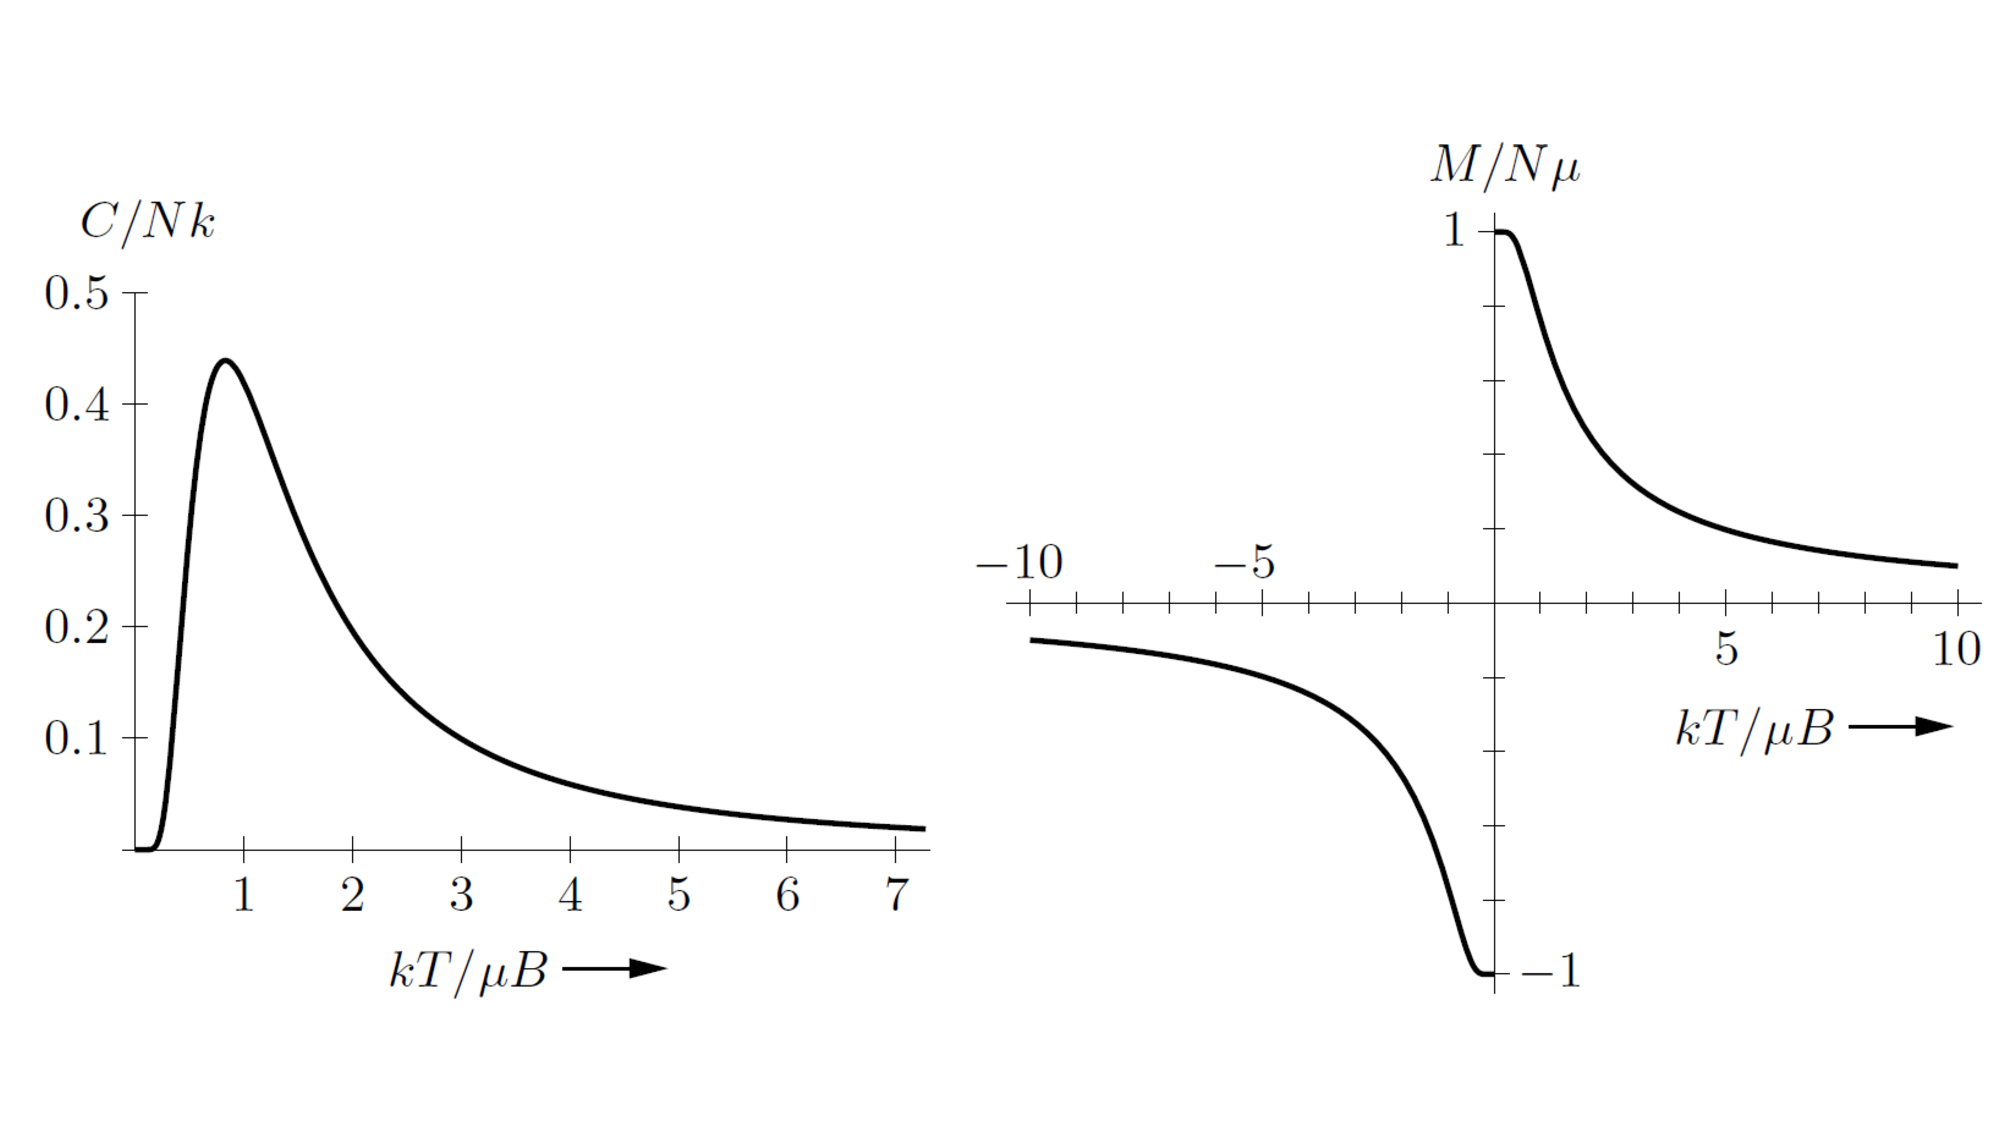
\includegraphics[width=0.9\linewidth]{imgs/Magnetic.pdf}
    \caption{Heat capacity and magnetization of a two-state paramagnet (computed
from the analytic formulas derived later in the text). Copyright 2000,
Addison-Wesley.}
    \label{fig:results}
\end{figure}

\section{Analytic solution}
We can also use Stirling's approximation to understand it analytically.
\begin{equation} 
\begin{split}
    S/k & = \ln N! - \ln N_\uparrow ! - \ln (N-N_\uparrow)! \\
        & \approx \ln N - N - N_\uparrow \ln N_\uparrow + N_\uparrow - (N-N_\uparrow)\ln(N-N_\uparrow) + (N-N_\uparrow) \\
        & = N\ln N - N_\uparrow \ln N_\uparrow - (N-N_\uparrow) \ln(N-N_\uparrow)
\end{split}
\end{equation}

To find the temperature relation, we need to differentiate $S$ with respect to $U$.
\begin{equation}
 \frac{1}{T} = \bigg(\frac{\partial S}{\partial U}\bigg)_{N, B} 
             = \frac{\partial N_\uparrow}{\partial U} \frac{\partial S}{\partial N_\uparrow} 
             = -\frac{1}{2\mu B}\frac{\partial S}{\partial N_\uparrow}    
\end{equation}
Now we get
\begin{equation}
    \frac{1}{T} = \frac{k}{2\mu B} \ln \frac{N-U/\mu B}{N+U/\mu B}
\end{equation}

Therefore, 
\begin{equation}
    U = N\mu B\frac{1-e^{2\mu B/kT}}{1+e^{2\mu B/kT}} = -N\mu B\tanh \bigg({\frac{\mu B}{kT}}\bigg)
\end{equation}
and the magnetization is
\begin{equation}
    M = N\mu\tanh \bigg({\frac{\mu B}{kT}}\bigg)
\end{equation}



To calculate the heat capacity of the paramagnet, we just need to differentiate the equation with respect to $T$;
\begin{equation}
    C_B = \bigg(\frac{\partial U}{\partial T}\bigg)_{N, B} = Nk \frac{(\mu B/kT)^2}{\cosh^2(\mu B/kT)}
\end{equation}
This function approaches zero at both high T and low T. 

At room temperature $\mu B = 5.8 \times 10^{-5}$ eV, while $kT$ is about 1/40 eV. So, we can assume that $\mu B/kT \ll 1$. In this limit, $\tanh(x) \approx x$, so the magnetization becomes 
\begin{equation}
    M \approx \frac{N\mu^2B}{kT}
\end{equation}

The fact that $M \propto 1/T$ was discovered by Pierre Curie and is known as \textbf{Curie's law}. 


\section{Homework}
Problem 3.19, 3.22, 3.23


\lecture{13}{Engines and Refrigerators}{Qiang Zhu}{scribe-name1,2,3}

\section{Heat Engines and Refrigerators}
A heat engine is any device that absorbs heat and converts part of that energy into work. Unfortunately, only part of the energy absorbed as heat can be converted to work. The reason is that the heat, as it flows in, brings along entropy, which must somehow be disposed as waste. 

\begin{figure}[ht]
\centering
\begin{tikzpicture}[thick]
\draw (0, -2.0) -- ( 0, 2.0) -- (4, 2.0) -- (4,-2.0) -- (0,-2.0);
\draw (-1, 2.1) -- (-1, 3.6) -- (5, 3.6) -- (5, 2.1) -- (-1, 2.1);
\draw (-1,-2.1) -- (-1,-3.6) -- (5,-3.6) -- (5,-2.1) -- (-1,-2.1);

\node at (1.8,2.8) {Hot reservoir, $T_h$};
\node at (1.8,-2.8) {Cold reservoir, $T_c$};
\node at (-1, 0) {Engine};
\draw [->,line width=0.1cm] (4, 0) -- (5.5,0) node [right]{$W$};
\draw [->,line width=0.1cm] (2, 2) -- (2,1) node  [below]{$Q_h$};
\draw [->,line width=0.1cm] (2,-1) -- (2,-2) node [below]{$Q_c$};

\draw (10,-2.0) -- (10, 2.0) -- (14, 2.0) -- (14,-2.0) -- (10,-2.0);
\draw ( 9, 2.1) -- ( 9, 3.6) -- (15, 3.6) -- (15, 2.1) -- ( 9, 2.1);
\draw ( 9,-2.1) -- ( 9,-3.6) -- (15,-3.6) -- (15,-2.1) -- ( 9,-2.1);

\node at (11.8,2.8) {Hot reservoir, $T_h$};
\node at (11.8,-2.8) {Cold reservoir, $T_c$};
\node at ( 8.5, 0) {Refrigerator};
\draw [<-,line width=0.1cm] (14, 0) -- (15.5,0) node [right]{$W$};
\draw [<-,line width=0.1cm] (12, 2) -- (12,1) node [below]{$Q_h$};
\draw [<-,line width=0.1cm] (12,-1) -- (12,-2) node [below]{$Q_c$};

\end{tikzpicture}
\caption{The schemes of cold and heat engines.}
\end{figure}

The benefit of a heat engine is the work produced, $W$. Let's define the efficiency $e$,
\begin{equation} e = \frac{W}{Q_h} \end{equation}
Because of the 1st law,
\begin{equation} Q_h = Q_c + W \end{equation}
\begin{equation} e = \frac{Q_h-Q_c}{Q_h} = 1 - \frac{Q_c}{Q_h} \end{equation}

According to the definition of entropy,
\begin{equation}    S2 \geq S1              ~~~~~~\rightarrow~~~~~~~ 
       \frac{Q_c}{T_c} \geq \frac{Q_h}{T_h} ~~~~~~\rightarrow~~~~~~~
       \frac{Q_c}{Q_h} \geq \frac{T_c}{T_h} 
\end{equation}
Therefore, we conclude
\begin{equation} e \leq 1-\frac{T_c}{T_h} \end{equation}


\section{Refrigerator}
The benefit of a refrigerator is $Q_c$. Let's define the efficiency $e$,
\begin{equation} e = \frac{Q_c}{W} \end{equation}
Because of the 1st law,
\begin{equation} Q_h = Q_c + W \end{equation}
\begin{equation} e = \frac{Q_c}{Q_h-Q_c} = \frac{1}{Q_h/Q_c-1} \end{equation}

According to the entropy relation,
\begin{equation}    S2 \geq S1              ~~~~~~\rightarrow~~~~~~~ 
       \frac{Q_c}{T_c} \geq \frac{Q_h}{T_h} ~~~~~~\rightarrow~~~~~~~
       \frac{Q_c}{Q_h} \geq \frac{T_c}{T_h} 
\end{equation}
Therefore, we conclude
\begin{equation} e \leq \frac{1}{T_h/T_c-1} \end{equation}

\section{To calculate the efficiency}
Suppose 1 mol He undergoes the following cycles, in which $P_2$ = 2$P_1$, $V_4$=2$V_1$. Calculate 
the heat transfer ($Q$) for each step, and the efficiency of the engine.\\

\begin{tikzpicture}[x=2cm, y=2cm]
\draw [->] (0,0) -- (2,0) node[below]{$V$};
\draw [->] (0,0) -- (0,2) node[above]{$P$};
\draw [->] (1,1) -- (1,2) node[above]{$P2,V2$}; 
\draw [->] (1,2) -- (2,2) node[above]{$P3,V3$};
\draw [->] (2,2) -- (2,1) node[above]{$P4,V4$}; 
\draw [->] (2,1) -- (1,1) node[above]{$P1,V1$}; 
\end{tikzpicture}


\section{The Carnot Cycle}
How to avoid an increase in entropy?\\
In order to avoid entropy's increase, we need to \\
1. keep $T_h$ = $T_\text{gas}$ and $T_c$ = $T_\text{gas}$ during heat transfer;\\
2. In the course of temperature dropping from $T_h$ and $T_c$, we use adiabatic conditions to avoid heat waste.
\begin{figure}[ht]
\centering
\begin{tikzpicture}[x=6cm, y=8cm]
\draw [->] (1.4, 0.5) -- (3.2, 0.5) node[below]{$V$};
\draw [->] (1.4, 0.5) -- (1.4, 1.3)  node[above]{$P$};
\draw [->, line width=0.05cm, blue, domain=1.67:2.0]  plot(\x, {  2.0/\x})           node[above, yshift=0.5cm] {isothermal};
\draw [->, line width=0.05cm, black,domain=2.00:3.0]  plot(\x, {2.639/((\x)^(1.4))}) node[above, yshift=0.2cm] {adiabatic};
\draw [->, line width=0.05cm, blue, domain=3.0:2.50]  plot(\x, {1.701/\x})           node[below, yshift=-0.2cm] {isothermal};
\draw [->, line width=0.05cm, black,domain=2.5:1.67]  plot(\x, {2.453/((\x)^(1.4))}) node[below, yshift=-0.9cm] {adiabatic};
\end{tikzpicture}
\caption{The Carnot cycle.}
\end{figure}

{\bf Exercises}\\
\begin{enumerate}
\item Why must you put an air conditioner in the window of a building, rather than in the middle of a room?
\item Can you cool off your kitchen by leaving the refrigerator door open?
\item Prove that the efficiency of a Carnot engine is 1-$\frac{T_c}{T_h}$
\end{enumerate}

\section{Homework}
Problem 4.2, 4.3, 4.11




\lecture{14}{Engines and Refrigerators}{Qiang Zhu}{scribe-name1,2,3}



\section{Real Heat Engines}
In the previous lecture, we have learned the theoretical limit of heat engines.
It is useful to know the upper limit when we design the engine.
However, one might also ask how it work in reality.
Can we follow the Carnot cycle in practice?

Now, let's discuss a few of engines used in real world.

\begin{figure}[ht]
\centering
\begin{tikzpicture} %[x=8cm, y=4cm]
\draw [->] (-0.5, -0.5) -- (5.0,-0.5) node[below]{$V$};
\draw [->] (-0.5, -0.5) -- (-0.5, 2.5)  node[above]{$P$};
\draw [->, line width=0.05cm, black,domain=3.0:1.5]  plot(\x, {1/((\x)^(1.4))}) node[below, xshift=0.1cm, yshift=-0.2cm] {1, Compression};
\draw [->, line width=0.05cm, blue] (1.5,0.567) -- (1.5,2.267)  node[left, yshift=-1cm]                                  {2, Ignition};
\draw [->, line width=0.05cm, black,domain=1.5:3.0]  plot(\x, {4/((\x)^(1.4))}) node[above, xshift=-0.4cm, yshift=0.5cm] {3, Power};
\draw [->, line width=0.05cm, blue] (3.0,0.859) -- (3.0,0.215)  node[right, yshift=0.4cm]                                {4, Exhaust};
\node at (1.5, -1) {$V_2$};
\node at (3.0, -1) {$V_1$};
\node  at (1.5, 3) {\large Otto cycle};

\draw [->] (9.0,-0.5) -- (14.0, -0.5) node[below]{$V$};
\draw [->] (9.0,-0.5) -- ( 9.0, 2.5) node[above]{$P$};
\draw [->, line width=0.05cm, black,domain=13.0:10.5]  plot(\x, {1/(\x-10)}) node[below, xshift=0.2cm, yshift=-1.5cm] {1, Compression};
\draw [->, line width=0.05cm, blue] (10.5,2.0) -- (11.5,2.0)  node[above, xshift=-0.8cm]                              {2, Ignition};
\draw [->, line width=0.05cm, black,domain=11.5:13.0]  plot(\x, {3/(\x-10)}) node[above, xshift=-0.5cm, yshift=0.5cm] {3, Power};
\draw [->, line width=0.05cm, blue] (13.0,1.0) -- (13.0,0.333)  node[right, yshift=0.4cm]                             {4, Exhaust};
\node at (10.5, -1) {$V_2$};
\node at (11.5, -1) {$V_3$};
\node at (13.0, -1) {$V_1$};
\node at (11.0, 3) {\large Diesel cycle};
\end{tikzpicture}
\caption{The Otto cycle and Diesel cycle.}
\end{figure}

Recall what we learned about P-V diagram in compression work, we can trivially derived the efficiency as a function of $V$
\begin{equation}
PV^{\gamma} = \text{const} ~~~~\rightarrow~~~~~~ e = 1-(\frac{V_2}{V_1})^{\gamma-1} 
                                                   = 1-\frac{T_1}{T_2} 
                                                   = 1-\frac{T_3}{T_4}~~~~~~~~~~~~~ \text{(Otto cycle)}
\end{equation}
\begin{equation}
PV = \text{const} ~~~~\rightarrow~~~~~~ e = 1-\frac{V_2}{V_1}  ~~~~~~~~~~~~~ \text{(Diesel cycle)}
\end{equation}
\\
\begin{figure}[ht]
\centering
\begin{tikzpicture} %[x=8cm, y=4cm]
\draw [->] (-0.5, -0.5) -- (5.0,-0.5) node[below]{$V$};
\draw [->] (-0.5, -0.5) -- (-0.5, 2.5)  node[above]{$P$};
\draw [->, line width=0.05cm, black,domain=1.5:3.0] plot(\x, {4/\x}) node[below, xshift=-0.2cm, yshift=1cm] {1, Expansion};
\draw [->, line width=0.05cm, blue] (3.0,1.333) -- (3.0,0.667)  node[right, yshift=0.5cm]                    {2, Heat removal};
\draw [->, line width=0.05cm, black,domain=3.0:1.5] plot(\x, {2/\x}) node[above, xshift=0.2cm, yshift=-1cm] {3, Compression};
\draw [->, line width=0.05cm, blue] (1.5,1.3333) --(1.5,2.667)  node[left, yshift=-0.8cm]                   {4, Heat addition};
\node at (1.5, -1) {$V_2$};
\node at (3.0, -1) {$V_1$};
\end{tikzpicture}
\caption{The idealized Stirling cycle.}
\end{figure}



Discussion on Stirling Engines
\\\\\\\\\\\\\\\\\\\\\\\\
\section{Steam Engines and Real Refrigerators}
A very different type of engine is the steam Engine, in which the liquid water/steam were used as the work substance.
It works as follows,
\begin{enumerate}
\item water is pumper to high pressure at nearly constant volume;
\item water flows into a boiler at constant pressure condition, then becomes steam;
\item steam hit the turbine, where it expands adiabatically, cools, ends up at the original pressure;
\item the fluid is cooled further to become water.
\end{enumerate}

On the other hand, refrigerator works as follows,
\begin{enumerate}
\item gas is compressed to adiabatically;
\item gives up heat and become liquids at constant pressure;
\item passes through a Throttle valve to 
\item absorbs heat and turns back to a gas in the evaporator
\end{enumerate}
\begin{figure}[ht]
\centering
\begin{tikzpicture} %[x=8cm, y=4cm]
\draw [->] (-0.5, -0.0) -- (5.0,-0.0) node[below]{$V$};
\draw [->] (-0.5, -0.0) -- (-0.5, 2.5)  node[above]{$P$};
\draw [->, line width=0.05cm]  (1.5,1.000) -- (1.5,2.267)  node[left,  yshift=-0.5cm]                                 {1, pump};
\draw [->, line width=0.05cm]  (1.5,2.267) -- (2.5,2.267)  node[above, xshift=-0.5cm]                               {2, boiler};
\draw [->, line width=0.05cm,domain=2.5:4.486]  plot(\x, {8.176/((\x)^(1.4))}) node[above, xshift=-0.4cm, yshift=0.5cm] {3, turbine};
\draw [->, line width=0.05cm] (4.486,1.000) -- (1.5,1.000)  node[below, xshift=0.8cm]                               {4, condenser};
\node  at (1.5, 3.5) {\large Rankine cycle};

\draw [->] (9.5, -0.0) -- (15.0,-0.0) node[below]{$V$};
\draw [->] (9.5, -0.0) -- (9.5, 2.5)  node[above]{$P$};
\draw [<-, line width=0.05cm]  (12.0,1.000) -- (11.5,2.267)  node[left,  yshift=-0.5cm]                                 {4, pump};
\draw [<-, line width=0.05cm]  (11.5,2.267) -- (12.5,2.267)  node[above, xshift=-0.5cm]                                 {3, condenser};
\draw [<-, line width=0.05cm,domain=12.5:14.486]  plot(\x, {8.176/((\x-10)^(1.4))}) node[above, xshift=-0.4cm, yshift=0.5cm] {2, compressor};
\draw [<-, line width=0.05cm] (14.486,1.000) -- (12.0,1.000)  node[below, xshift=0.8cm]                               {1, evaporator};
\node at (12.0, 3.5) {\large Refrigeration cycle};
\end{tikzpicture}
\caption{The Rankine cycle and Refrigeration cycle.}
\end{figure}

\begin{equation}
e = 1-\frac{Q_c}{Q_h} = 1-\frac{H_4-H_1}{H_3-H_2} = 1-\frac{H_4-H_1}{H_3-H_1}
\end{equation}

\begin{equation}
\text{COP} = \frac{Q_c}{Q_h-Q_c} = \frac{H_1-H_4}{H_2-H_3-H_1+H_4} 
\end{equation}

\section{Homework}
Problem 4.18, 4.21, 4.26, 4.27, 4.36



\lecture{15}{Free Energy}{Qiang Zhu}{scribe-name1,2,3}

\section{Outline}
In the previous chapter, we applied the laws of thermodynamics to study cyclic processes. Now let's turn to chemical reactions and other phase transformations of matter. One complication is that the system usually involves interactions with its surroundings, in thermal, mechanical, chemical ways. Therefore, energy is not conserved in these cases. Instead, $T$, $P$, $\mu$ become crucial parameters.

\section{Free Energy}
The first task is to develop the conceptual tools needed to understand constant $T$, $P$ processes.
Recall we have defined the concept of enthalpy ($H$),
\begin{equation} \label{entropy} 
H \equiv U + PV
\end{equation}
Let's understand it in this way. If you could completely annihilate the system, $H$ is the energy cost you need to pay.
In addition to its internal energy ($U$), you also need to plus $PV$ work.

Similarly, we have two more useful quantities that are related to energy and analogous to $H$,
\begin{equation} \label{entropy} 
F \equiv U - TS    ~~~~~~~~~ \text{(Helmholtz free energy, constant temperature )}
\end{equation}

\begin{equation} \label{entropy} 
G \equiv U - TS + PV   ~~~~~~~~~ \text{(Gibbs free energy, constant temperature, constant pressure )}
\end{equation}

The four functions $U, H, F, G$ are collectively called thermodynamic potentials. Their relations are shown as follows,
\begin{figure}[h]
\centering
\begin{tikzpicture}[thick]
\draw (0,0) -- (2,0);
\draw (0,1) -- (2,1);
\draw (0,2) -- (2,2);
\draw (0,0) -- (0,2);
\draw (1,0) -- (1,2);
\draw (2,0) -- (2,2);
\node at (0.5,0.5) {$H$};
\node at (1.5,0.5) {$G$};
\node at (0.5,1.5) {$U$};
\node at (1.5,1.5) {$F$};
\node at (1.0,2.2) {$-TS$};
\node at (-1.0,1.0) {$+PV$};

\end{tikzpicture}
\end{figure}

\section{How to measure $\Delta{G}$}
The easiest way is,
\begin{enumerate}
\item measure the heat absorbed when the reaction takes place, $\Delta{H}$;
\item calculate $\Delta{S}$ according to the heat capacities $C_P$ and the initial/final temperature;
\item $\Delta{G}$ = $\Delta{H}$ - $T\Delta{S}$
\end{enumerate}
Consider the production of ammonia from nitrogen and hydrogen at 298 K and 1 bar, \\
\ce{N2(g) + 3H2(g) -> 2NH3(g)}\\\\
From the values of $\Delta{H}$ and S, compute $\Delta{G}$ for this reaction and check that it is consistent with the value given in the table.\\\\\\\\


\section{Electrochemical Reactions}
Consider the chemical reaction of the electrolysis of water to hydrogen and oxygen gas,\\\\
\ce{H2O(l) -> H2(g) + 1/2O2(g)}\\\\
\begin{tabular}{|c | c | c | c | c |}
\hline
Type                 &  H$_2$O(l)& H$_2$(g)& O$_2$(g)&   Total  \\\hline
$\Delta{H}$(kJ)      &  -285.8   &    0    &   0     &   285.8  \\\hline
$S$ (J/K)            &    69.9   & 130.7   & 205.1   &  -163.4  \\\hline
$P\Delta{V}$(kJ)     &           &         &         &     3.7  \\\hline
$\Delta{U}$(kJ)      &           &         &         &   282.1   \\\hline
$T\Delta{S}$(kJ)     &           &         &         &   -48.3  \\\hline
$\Delta{G}$(kJ)      &           &         &         &   237.1  \\\hline
\end{tabular}

The reverse reaction is the combustion of hydrogen gas, a reaction that might replace the internal combustion engine in future automobiles (fuel cell).
In the process of producing the electric work, the fuel cell will also dump 49 kJ of waste heat.
But the waste heat is only 17\% of heat generated from this reaction. So an ideal hydrogen fuel cell has an `efficiency' of 83\%, much better than any practical engine.


%Another good example is the electric energy output of a battery.\\\\
%\ce{Pb + PbO2 + 4H{+} + 2SO4^{2-} -> 2PbSO4 + 2H2O}\\\\
%\begin{tabular}{|c | c | c | c | c | c | c | c |}
%\hline
%Type                 &   Pb      &  PbO$_2$& H$^{+}$ &   SO$_4^{2-}$ &PbSO$_4$ & H$_2$O(l) & Total \\\hline
%$\Delta{H}$(kJ)      &           &         &         &               &         &           & \\\hline
%$S$ (J/K)            &           &         &         &               &         &           & \\\hline
%$P\Delta{V}$(kJ)     &           &         &         &               &         &           & \\\hline
%$\Delta{U}$(kJ)      &           &         &         &               &         &           &  \\\hline
%$T\Delta{S}$(kJ)     &           &         &         &               &         &           & \\\hline
%$\Delta{G}$(kJ)      &           &         &         &               &         &           & \\\hline
%\end{tabular}


\section{Thermodynamic Identities}
In the previous chapter, we already learned
\begin{equation} dU = TdS - PdV + \mu dN \end{equation}
What will happen on $H$, $F$, $G$?

\begin{equation} 
\begin{split}
dH  = &  dU + PdV + VdP   \\
    = & TdS + VdP + \mu dN 
\end{split}
\end{equation}

Similarly, we could derive that 
\begin{equation} 
\begin{split}
dF  = &  dU - (TdS + SdT)   \\
    = & -SdT  - PdV + \mu dN 
\end{split}
\end{equation}

\begin{equation} 
\begin{split}
dG  = & dF + PdV + VdP   \\
    = & -SdT + VdP + \mu dN 
\end{split}
\end{equation}

Accordingly, we can derive the partial derivatives from $G$,
\begin{equation} S   = -(\frac{\partial {G}}{\partial {T}})_{P,N} \end{equation}
\begin{equation} V   = (\frac{\partial {G}}{\partial {P}})_{T,N} \end{equation}
\begin{equation}\mu  = (\frac{\partial {G}}{\partial {N}})_{T,P} \end{equation}


\section{Maxwell Relation}
Functions encountered in physics are generally well enough behaved that their
mixed partial derivatives do not depend on which derivatives are taken first. For instance,
\begin{equation} 
                 \frac {\partial}{\partial V} (\frac{\partial U}{\partial S}) 
               = \frac {\partial}{\partial S} (\frac{\partial U}{\partial V})
\end{equation}
From the thermodynamic identities (for $U$), we can evaluate the partial derivatives,
\begin{equation} 
               (\frac{\partial T}{\partial V})_S
               = -(\frac{\partial P}{\partial S})_V
\end{equation}
Similarly, we apply it on $H$,$F$,$G$,
\begin{equation} \frac {\partial}{\partial P} (\frac{\partial H}{\partial S}) 
               = \frac {\partial}{\partial S} (\frac{\partial H}{\partial P})
               ~~~ \rightarrow ~~~~
                (\frac{\partial T}{\partial P})_S
               = (\frac{\partial V}{\partial S})_P
\end{equation}
\begin{equation} \frac {\partial}{\partial V} (\frac{\partial F}{\partial T}) 
               = \frac {\partial}{\partial T} (\frac{\partial F}{\partial V})
               ~~~ \rightarrow ~~~~
                (\frac{\partial S}{\partial V})_T
               = (\frac{\partial P}{\partial T})_V
\end{equation}
\begin{equation} \frac {\partial}{\partial P} (\frac{\partial G}{\partial T}) 
               = \frac {\partial}{\partial T} (\frac{\partial G}{\partial P})
               ~~~ \rightarrow ~~~~
                (\frac{\partial S}{\partial P})_T
               = -(\frac{\partial V}{\partial T})_P
\end{equation}

These are {\bf Maxwell relations}. It is useful because it could quantify the changes of 
entropy which are not directly measurable, in terms of measurable quantities like $T,V,P$.
Here let me just give some of its applications.
The thermal expansion coefficient is defined as follows,
\begin{equation}
\beta = \frac{\Delta{V}/V}{\Delta{T}} = -\frac{1}{V}(\frac{\partial V}{\partial T})_P
\end{equation}
Plugging in the Maxwell relation,
\begin{equation}
\beta = \frac{1}{V}(\frac{\partial V}{\partial T})_P 
      = \frac{1}{V}(\frac{\partial S}{\partial P})_T 
\end{equation}

According to the 3rd law, entropy approaches to 0 or some constant regardless of $P$. Hence $\beta$ = 0 when $T$ goes to 0.

Now let's dig into the difference between $C_V$ and $C_P$
\begin{equation}
dS = (\frac{\partial{S}}{\partial{T}})_V dT + (\frac{\partial{S}}{\partial{V}})_T dV
\end{equation}

\begin{equation}
dV = (\frac{\partial{V}}{\partial{T}})_p dT + (\frac{\partial{V}}{\partial{P}})_T dP
\end{equation}

\begin{equation}
(dS)_P = (\frac{\partial{S}}{\partial{T}})_V dT + (\frac{\partial{S}}{\partial{V}})_T (\frac{\partial{V}}{\partial T})_P dT
\end{equation}
That is,
\begin{equation}
(\frac{\partial S}{\partial T})_P = (\frac{\partial{S}}{\partial{T}})_V + (\frac{\partial{S}}{\partial{V}})_T (\frac{\partial{V}}{\partial T})_P
\end{equation}

\begin{equation}
C_P = C_V + T(\frac{\partial{S}}{\partial{V}})_T (\frac{\partial{V}}{\partial T})_P
\end{equation}

\begin{equation}
C_P = C_V + T(\frac{\partial{P}}{\partial{T}})_V (\frac{\partial{V}}{\partial T})_P
\end{equation}

from problem 1.46,
\begin{equation}
(\frac{\partial{P}}{\partial{T}})_V = -\frac{(\partial{V}/{\partial T})_P}{(\partial{V}/{\partial P})_T}
\end{equation}

Therefore,
\begin{equation}
C_P = C_V - T(\frac{\partial{V}}{\partial{T}})^2_P / (\frac{\partial{V}}{\partial P})_T
\end{equation}

Recall the definition of $\beta$ and $\kappa$
\begin{equation}
\beta = \frac{1}{V}(\frac{\partial{V}}{\partial{T}})_P;~~~~~~ \kappa_T = -\frac{1}{V}(\frac{\partial{V}}{\partial{P}})_T
\end{equation}

\begin{equation}
C_P - C_V = -T(\beta V)^2/(-\kappa_T V) = \frac{TV\beta^2}{\kappa_T}
\end{equation}




\lecture{16}{Free Energy}{Qiang Zhu}{scribe-name1,2,3}

\section{Free Energy as a Force toward Equilibrium}
For an isolated system, the entropy tends to increase. The system's entropy determines the direction of spontaneous change. 
But what if a system is not isolated? Now energy can pass between the system and the environment. The 2nd law still applies.
However, the total entropy would be the determining factor.

Let's consider a small change in the total entropy;
\begin{equation} dS_\text{total} = dS + dS_R \end{equation}

Applying the thermodynamic identity, we get,
\begin{equation} dS = \frac{1}{T}dU + \frac{P}{T}dV - \frac{\mu}{T}dN \end{equation}

if we assume $N$ and $V$ is fixed, we have
\begin{equation} dS_\text{total} = dS + \frac{1}{T}dU_R \end{equation}
Since $T$ is in equilibrium,
\begin{equation} dS_\text{total} = dS - \frac{1}{T}dU \end{equation}
Therefore,
\begin{equation} dS_\text{total} = -\frac{1}{T}(dU-TdS) = -\frac{1}{T}dF \end{equation}
Finally, we come to the conclusion that the increase of $S$ is equivalent to the decrease in $F$, under constant $N, V, T$ conditions.
This allows us to forget about the reservoir and just consider the free energy itself.
Similarly, we can derive the relation under constant $N, P, T$ conditions,
\begin{equation} dS_\text{total} = -\frac{1}{T}(dU-TdS+PdV) = -\frac{1}{T}dG \end{equation}

Let me summarize these points,
\begin{enumerate}
\item constant $V, T$ $\rightarrow$ $S$ tends to increase
\item constant $N, V, T$, $\rightarrow$ $F$ tends to decrease
\item constant $N, P, T$, $\rightarrow$ $G$ tends to decrease
\end{enumerate}

Reconsider the case of burning water:~~~~~~~\ce{H2 + 1/2 O2 -> H2O}\\

\section{Various Phase Transitions}
Phases: Different forms of the substance, such as liquid, gas, solid.\\
A phase transformation is a discontinuous change in the properties of a substance.\\
1st order $\rightarrow$ the discontinuous changes of properties is the 1st derivative of energy\\
2nd order $\rightarrow$ the discontinuous changes of properties is the 2nd derivative of energy\\
Some key points in the phase diagram,
\begin{enumerate}
\item phase boundary, 
\item triple point, where solid, liquid, gas coexists
\item slope of phase boundary, ice anomaly
\item critical points, where gas and liquid are no longer distinguishable (fluid)
\item superconducting......
\item Curie temperature
\end{enumerate}

Diamond/Graphite
\begin{equation} 
(\frac{\partial G}{\partial P})_{T,N} = V
\end{equation}

\begin{equation} 
(\frac{\partial G}{\partial T})_{P,N} = -S
\end{equation}



\section{The Clausius-Clapeyron Relation}
At the phase boundary, the material is equally stable as a liquid or a gas, so its Gibbs free energy must be the same,
\begin{equation} G_l = G_g \end{equation}
Now imagine increasing the temperature by $dT$ and the pressure by $dP$, in such a way that the two phases remain equally stable.
Under this change,
\begin{equation} dG_l = dG_g \end{equation}
Therefore, by the thermodynamic identify for $G$,
\begin{equation} -S_ldT + V_ldP = -S_gdT + V_gdP \end{equation}
Where $\mu dN$ term is intentionally neglected ($N$ is fixed). 
Now it is easy to solve for the slope of the phase boundary line,
\begin{equation} \frac{dP}{dT} = \frac{S_g-S_l}{V_g-V_l} \end{equation}
Therefore, the slope is determined by the entropies and volumes of the two phases.
Shallow/stiff.
In practice, it is more convenient to write as
\begin{equation} \frac{dP}{dT} = \frac{L}{T\Delta{V}} \end{equation}
where, $L$ is the latent heat for converting the material from liquid to gas. And this is known as the {\bf Clausius-Clapeyron relation}

The $P$-$T$ slope of the solid-liquid phase boundary is usually positive. But water is an exception. Why?\\
Diamond/Graphite, (300 K, 15 kbar) .v.s (1800 K, 60 kbar)\\

Below 0.3 K the slope of the $^3$He solid-liquid phase boundary is negative, which phase is more dense? Which phase has more entropy?\\
Solid phase is denser, and has more entropy.\\
At absolute 0 K, the slope goes to 0, as $\Delta{S}$ goes to 0.\\
From Liquid to Solid, $S$ has to increase.\\
During adiabatic compression, $S$ has to remain constant.\\
Therefore, $T$ has to drop. A good way to reach ultra-low temperature.

\section{Homework}
Problems 5.12, 5.13, 5.14, 5.21, 5.23\\
Problems 5.24, 5.28, 5.29, 5.32, 5.40\\
%{\bf Problem 5.45}, when a rising air mass becomes saturated, the condensing water droplets will give up energy, thus slowing the adiabatic cooling process. Use the first law to show that, as condensation forms during adiabatic expansion, the temperature of an air mass changes by
%\begin{equation}
%dT = \frac{2}{7}(\frac{T}{P}dP - \frac{L}{nR}dn_w,
%\end{equation}
%where $n_w$ is the number of moles of water vapor present, $L$ is the latent heat of vaporization per mol, and $\gamma$ is 7/5 for air. You may assume that the H$_2$O makes up only a small fraction of the air mass.
%
\newpage
\begin{figure}[h]
\centering
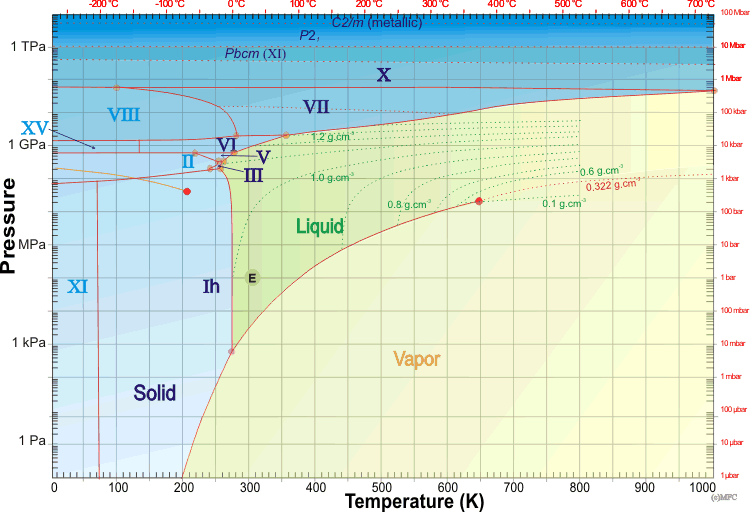
\includegraphics[width=12cm]{imgs/water_phase_diagram_2}
\caption{The Phase diagram for H$_2$O. }
\end{figure}

\begin{figure}[ht]
\centering
\begin{tikzpicture}%[x=1cm, y=3cm]
\draw [->] (0,0) -- (0, 3) node[above]{$G$};
\draw [->] (0,0) -- (5, 0)  node[below]{$P$};
\draw [color=blue, domain=0:5]  plot(\x, {0.39 + 0.342*\x}) node[below] {Diamond};
\draw [color=black,domain=0:5]  plot(\x, {0.10 + 0.531*\x}) node[above] {Graphite};
\end{tikzpicture}
\caption{Graphite versus diamond.}
\end{figure}



\lecture{17}{Phase Transitions, van der Waals Model}{Qiang Zhu}{scribe-name1,2,3}

\section{The van der Waals Model}
To understand phase transformations more deeply, 
\begin{enumerate}
\item What's the shape of phase boundary?
\item Why there is a critical point? What's its origin?
\end{enumerate}

we should start with a specific mathematical model.
The easiest model is perhaps to study liquid-gas transformations based van der Waals model.

In 1873, van der Waals proposed a modified model based on the ideal gas law.
\begin{equation} 
(P + \frac{\alpha N^2}{V^2})(V-Nb) = NkT
\end{equation}

The modifications are the following,
\begin{enumerate}
\item Subtracting $Nb$ from $V$, which accounts for the minimum volume when pressure goes to infinity. 
\item Adding $aN^2/V^2$ to $P$, which account for the short range attractive forces.
\end{enumerate}

Why $N$ and $N^2/V^2$?\\
Considering all atoms are spheres, the minimum of $V$ must be proportional to $N$.\\
The potential energy must be proportional to its density $N \times N/V$.\\

For convenience, we can express $P$ from the vdW equation as follows
\begin{equation} 
P = \frac{NkT}{V-Nb}-\frac{aN^2}{V^2}
\end{equation}

The constants of $a$ and $b$ must be fitted for different systems.
$b$ corresponds to the molecular volume. While $a$ is much more variable because of the complex intermolecular interactions.
Now let us investigate the consequence of the vdW model.
At high $T$ regime ($V$ goes to high), it exactly behaves like gas.
At low $T$ regime, the behavior is much more complicated. As $V$ decreases to the isotherm rises, falls, and then rises again.

At a given $P,T$, the true equilibrium state of a system is determined by its Gibbs free energy. To calculate $G$ for a vdW fluid, let's
start with the thermodynamic identity.
\begin{equation}
dG= -SdT + VdP + \mu dN
\end{equation}

For a fixed amount of materials, at a given temperature, thie equation reduces to $dG=VdP$. Dividing both sides by $dV$ gives,
\begin{equation}
(\frac{\partial G}{\partial V})_{N,T} = V (\frac{\partial P}{\partial V})_{N,T} 
\end{equation}
The right-hand side can be computed from the vdW model,
\begin{equation}
(\frac{\partial G}{\partial V})_{N,T} = - \frac{NkTV}{(V-Nb)^2} + \frac{2aN^2}{V^2}
\end{equation}

To integrate it, we obtain
\begin{equation}
G = -NkT\text{ln}(V-Nb) + \frac{(NkT)(Nb)}{V-Nb} - \frac{2aN^2}{V} + c(T)
\end{equation}

This equation allows us to plot the Gibbs free energy for any fixed $T$.

To understand it, let's try to make the plot of $G$ as a function of $P$ and $V$. From the $G-P$ plot, we can clearly see that there is a
triangle loop in the graph (2-3-4-5-6), corresponding to the unstable states. As the pressure gradually increases, the system will go 
straight from 2 to 6, with an abrupt decrease in volume. A phase transformation therefore occurs. At point 2, we call it a gas, but point 6 a liquid.
At intermediate volumes, the thermodynamically stable state is actually a combination of part gas and part liquid, as indicated by the straight
vertical line on the $P-V$ diagram. 

The pressure at the phase transformation is easy enough to determine from the graph of $G$, but there is a way to obtain it from the $PV$ graph.
Clearly, there should be zero net work during 2-3-4-5-6 loop, since 2, 6 are in equilibrium. This is called {\bf Maxwell construction}.

Repeating the Maxwell construction for a variety of temperatures gives the vapor pressures. The region which the line crosses defines the regions in the coexistence of liquid and gas.
However, what will happen on high temperature? There is no way to build Maxwell construction. Hence the phase boundary must disappear at some temperature, which we call it critical temperature, $Tc$.
And the corresponding $P,V$ is called $Pc$ and $Vc$. These values defines the {\bf critical point}. If the temperature goes beyond critical point, the liquid and gas are no longer distinguishable.
\begin{equation}
\frac{\partial P}{\partial V} = 0 ~~~~~~  \frac{\partial^2 P}{\partial V^2} = 0
\end{equation}

Prove the following relations
\begin{equation}
V_c = 3Nb ~~~~~~  P_c = \frac{1}{27} \frac{a}{b^2} ~~~~~~ kT_c = \frac{8}{27} \frac{a}{b}
\end{equation}

Homework 
Problem 5.48, 5.49, 5.51, 5.52, 5.53


\begin{figure}[h]
\centering
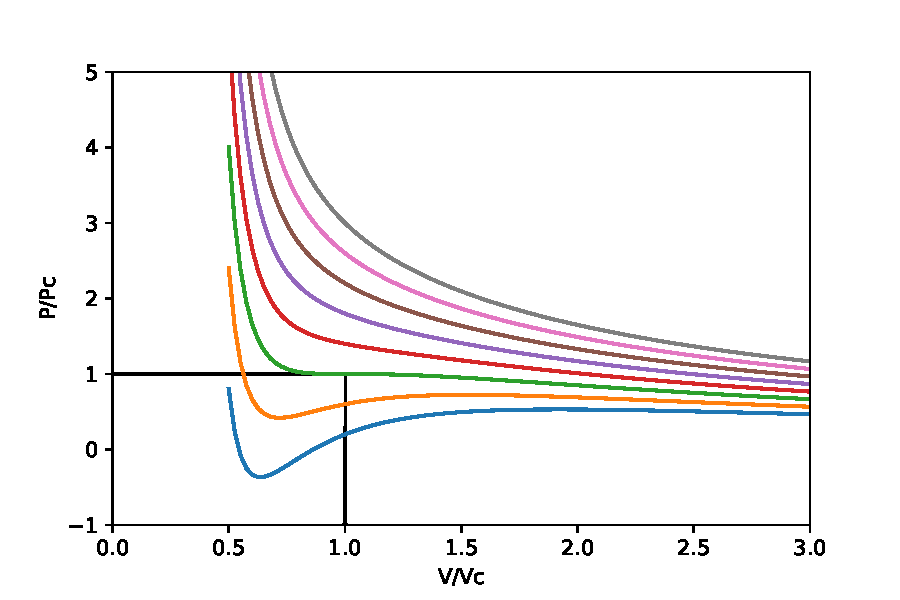
\includegraphics[width=9cm]{imgs/vdW.pdf}
\caption{$P-V$ isothermal curves close to the phase transition temperature. }
\end{figure}


\begin{figure}[h]
\centering
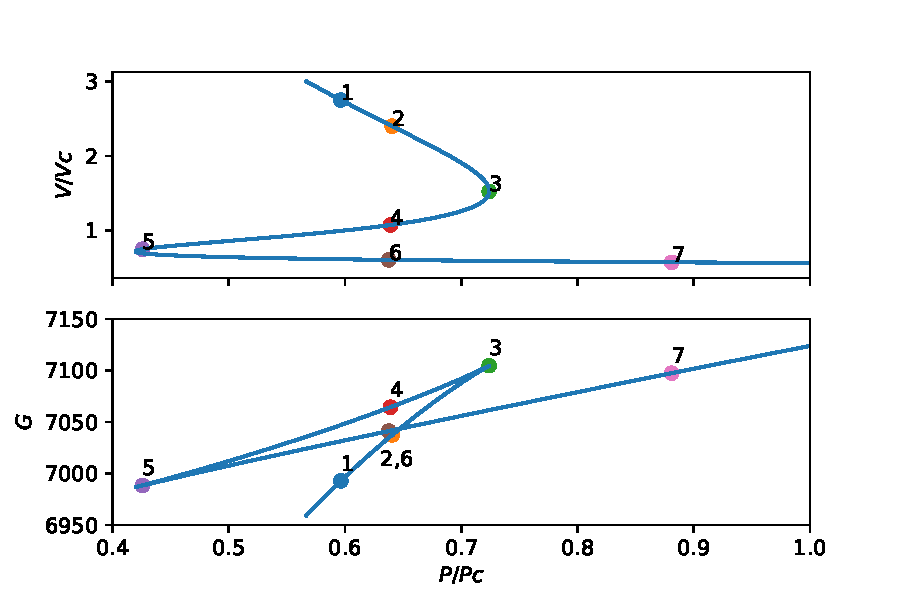
\includegraphics[width=9cm]{imgs/MaxWell.pdf}
\caption{Gibbs free energy as a function of pressure for a vdW model at $T$=0.9 Tc. The corresponding isotherm is shown at above.}
\end{figure}

\begin{figure}[h]
\centering
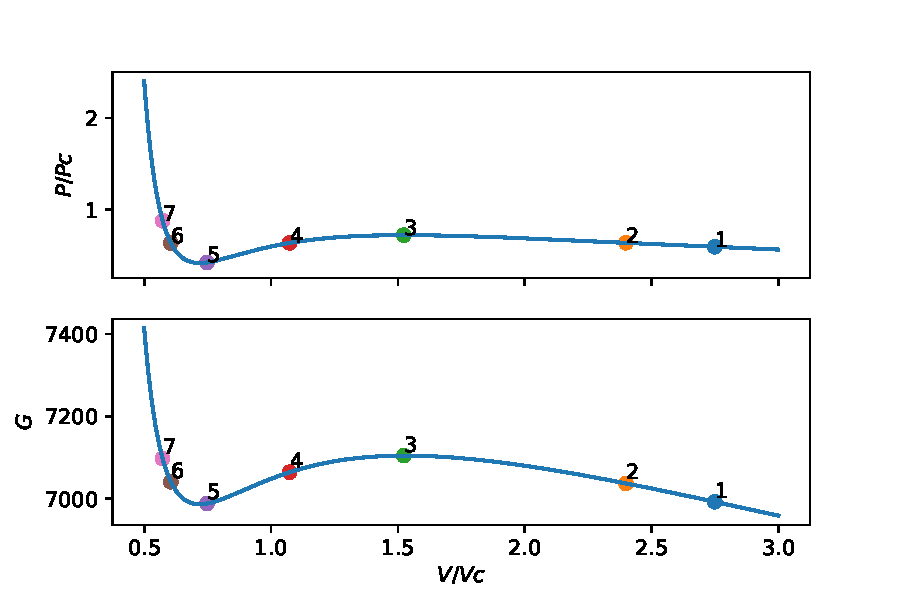
\includegraphics[width=9cm]{imgs/MaxWell-f.pdf}
\caption{Gibbs free energy as a function of volume for a vdW model at $T$=0.9 Tc. The corresponding isotherm is shown at above.}
\end{figure}



\lecture{18}{Phase Transformation of Mixtures}{Qiang Zhu}{scribe-name1,2,3}


\section{Free Energy of Mixture}
Phase Transformations become more complicated when a system contains two or more types of particles.
For example, what will happen if you lower the temperature of this mixture at 1 atm.
You might expect that all the oxygen will liquefy at 90.2 K, leaving a gas of pure nitrogen which 
would transform to liquid till 77.4 K. However, no liquid at all forms until the temperature drops to 81.6 K.
Similar behaviors happen on liquid-solid transition as well. How to understand it?

\begin{figure}[h]
\centering
\label{ideal-mix}
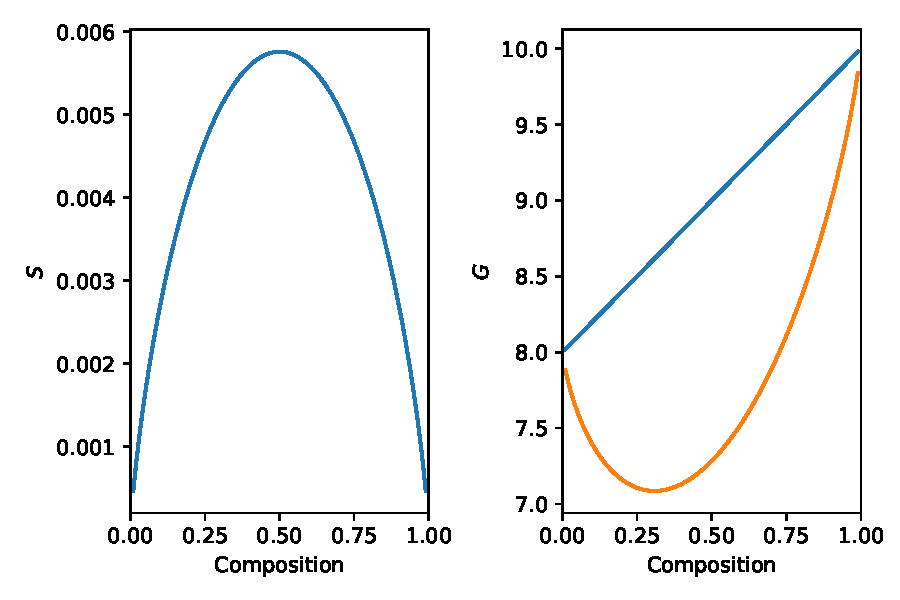
\includegraphics[width=12cm]{imgs/Ideal-Mixture.pdf}
\caption{The Phase diagram of ideal mixture, where $TS$ is the only term to contribute to $\Delta{G}$. }
\end{figure}


The key is to look at the Gibbs free energy as we did on vdW model. Let's consider a system of two molecules, $A$
and $B$, suppose that they are initially separated, sitting side by side at the same temperature and pressure. For
an unmixed system, the total free energy is just the sum of the two subsystems,
\begin{equation}
G = (1-x)G_A + xG_B,
\end{equation}
where $x$ is the fraction of $B$. 

Now suppose that we remove the partition between two sides and let them mix. From the definition of $G=U+PV-TS$.
\begin{enumerate}
\item $U$, depends on the intermolecular forces
\item $V$, depends on the forces as well
\item $S$, must increase according to what we learn in chapter 2.
\end{enumerate}

For the case of ideal gas (Fig. \ref{ideal-mix}), we can assume $U,V$ don't change.

Therefore the free energy of the mixture becomes,
\begin{equation}
G = (1-x)G_A + xG_B + RT[x\text{ln}x + (1-x)\text{ln}(1-x)]
\end{equation}

Note this only applies to ideal mixture. For real cases such as the mixing of liquids, it would usually cause the increase of $U$.

Let $n$ be the average number of the nearest neighbours, $\mu_0$ be the average potential energy of A-A or B-B interaction,
\begin{equation}
U = 1/2Nn\mu_0   
\end{equation}

If we mix it, the total potential energy then becomes,
\begin{equation}
\begin{split}
U &= 1/2[(1-x)N(xn\mu_\text{AB} + (1-x)n\mu_0) + xN(xn\mu_0 + (1-x)n\mu_\text{AB})] \\
  &= 1/2Nn([x^2+(1-x)^2]\mu_0 + 2x(1-x)\mu_\text{AB})
\end{split}
\end{equation}

Therefore,
\begin{equation}
\Delta{U} = Nnx(1-x)(\mu_{AB}-\mu_0)
\end{equation}

\begin{figure}[h]
\centering
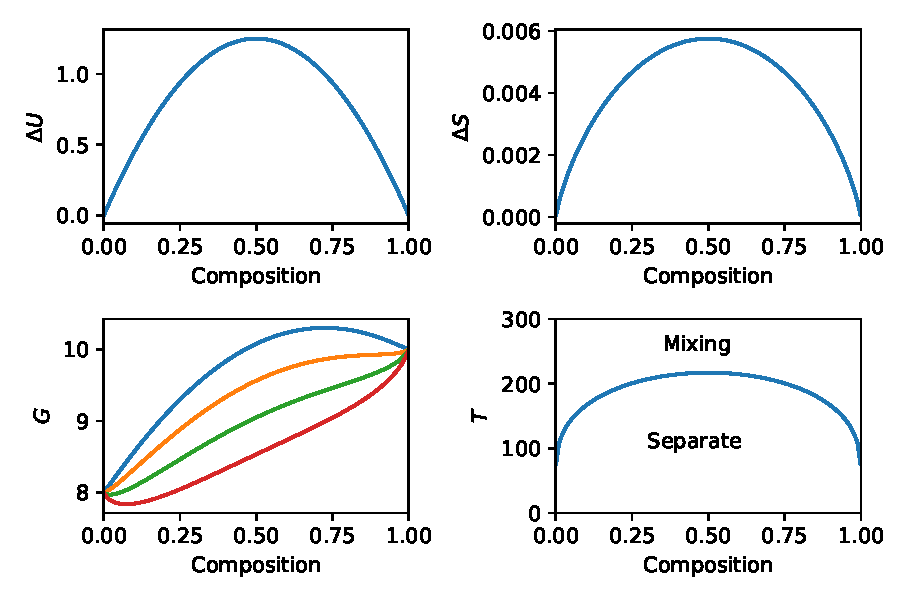
\includegraphics[width=12cm]{imgs/NonIdeal-Mixture.pdf}
\caption{The Phase diagram of non-ideal mixture, where only $\Delta{U}$ also contributes to $\Delta{G}$. When $\Delta{U}$ is positive, there exists 
a competition between $U$ and $TS$.}
\label{fig-non-ideal}
\end{figure}

The qualitative results are shown in Fig. \ref{fig-non-ideal}. If $\mu_{AB}$ is greater than $\mu_0$, it means $\Delta{U}$ favors the mixing. But it is not always the case. If $\mu_{AB}$ is smaller than $\mu_0$, there would be a competition between $U$ and $TS$. At low $T$, the shape is concave-down. At sufficiently high $T$, $TS$ becomes dominant, thus the shape is concave-up. But a concave-down free energy function indicates an unstable mixture. Therefore, we know $T$ determines if $\Delta{G}$ is positive or negative. For each given $x$ we can determine the critical temperature. Such a $T-x$ diagram could be very useful to help us identify which region the systems are miscible or not.

\begin{figure}[ht]
\centering
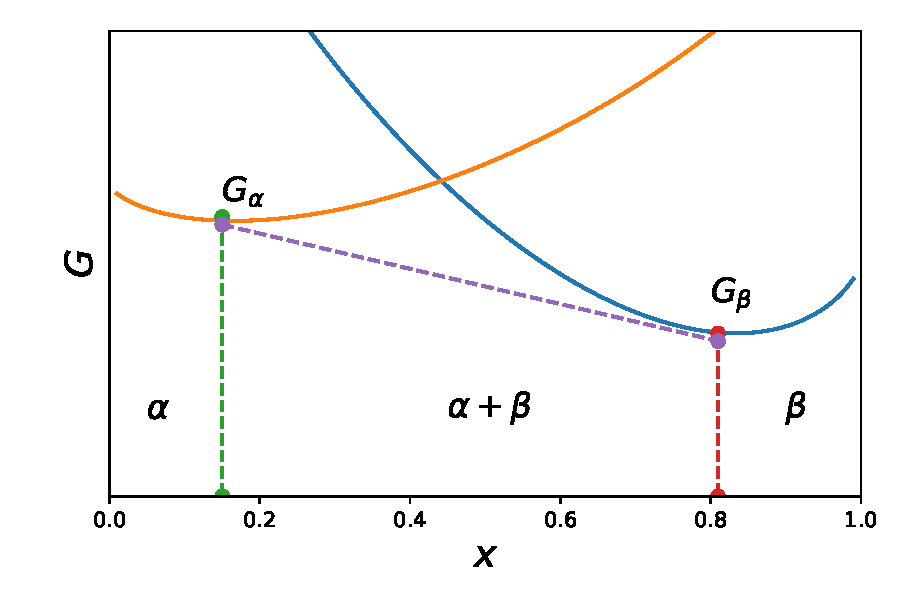
\includegraphics[width=10cm]{imgs/two-solids.pdf}
\label{fig-calc}
\caption{The Phase diagram of two systems which are not miscible to each other. In the intermediate region, the phase is a mixture of $\alpha$ and $\beta$.
This is called \textbf{solubility gap}.}
\end{figure}


\section{Phase diagram of a Miscible Mixture}
Let's come back to the problem of liquefy air. 
\begin{enumerate}
\item $T_A$, oxygen will start to liquefy at 90.2 K 
\item $T_B$, nitrogen will completely become liquid at 77.4 K. 
\item $T_A<T<T_B$, liquid and gas will coexist, depending on the ratio $x$.
\end{enumerate}

$G-x$ diagram\\
$T-x$ diagram\\
\begin{figure}[ht]
\centering
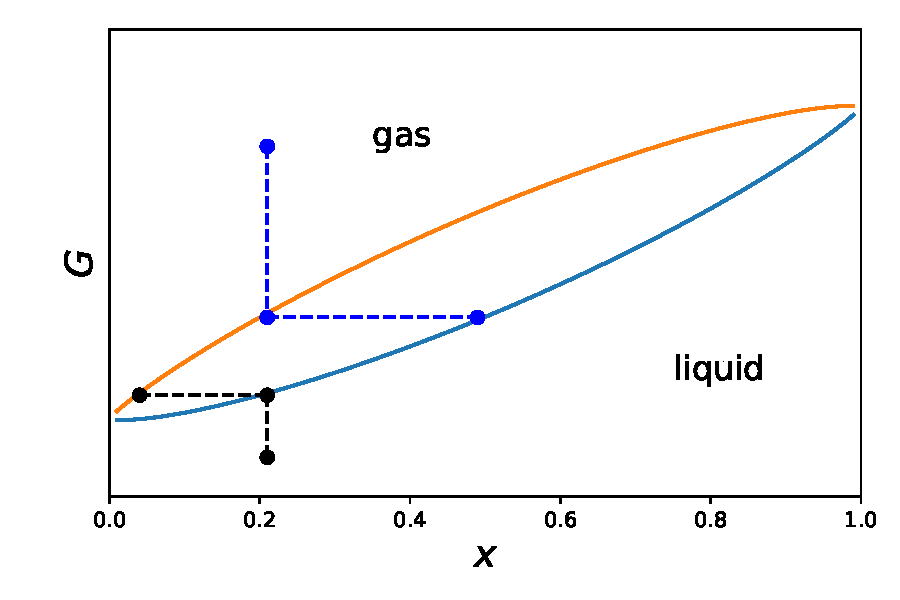
\includegraphics[width=10cm]{imgs/air.pdf}
\caption{The Phase diagram of air mixture.}
\end{figure}


\section{Phase Diagram of Eutectic Mixture}
Most two solids do not maintain the same crystal structures over the entire range of composition. If we consider the the solid-liquid transition with the possibility of two solid phases, this picture will become more complicated. Again the idea is to look at the free energy at various temperatures. Suppose $T_B$ is the melting point of B and $T_A$ is the melting point of A. 

\begin{enumerate}
    \item At high temperatures the free energy of the liquid will be below that of either solid phase. 
    \item As the temperature drops, all three energy functions will increase ($\frac{\partial G}{\partial T}=-S$), but the free energy of the liquid will increase fastest because it has higher $TS$ term. Below $T_B$ the liquid's free energy curve will intersect that of the B phase, so there is a range of compositions for which the stable configuration is an unmixed combination of liquid and B. 
    \item as T decreased further, this range reaches the A side of the diagram and you will find the range of an unmixed combination of liquid and A.
    \item if we drop the T further, we will find that A+liquid and B+liquid will meet at a particular point (\textbf{Eutectic point}). An Eutectic point defines the lowest melting point of the system. 
\end{enumerate}

\begin{figure}[ht]
\centering
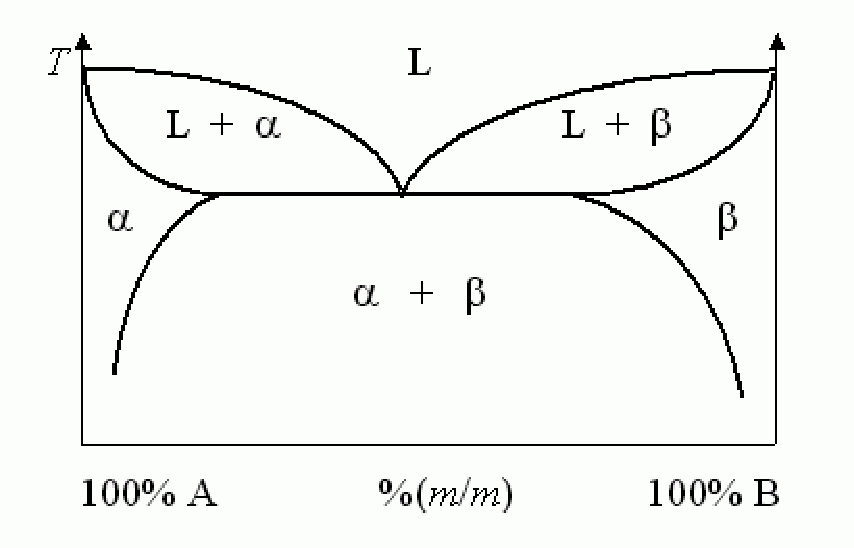
\includegraphics[width=10cm]{imgs/Eutectic.pdf}
\caption{The Phase diagram of A-B mixture.}
\end{figure}



\lecture{19}{Dilute Solutions}{Qiang Zhu}{scribe-name1,2,3}

A solution is similar to the case of a mixture. A solution is called \textit{dilute} if the concentration of solute is much less than the number of solvent molecules. In many ways the solute in a dilute solution behaves like an ideal gas. We can therefore predict many of the properties quantitatively.

\section{Solvent and Solute}
To make a prediction, we first need to know something about its chemical potentials. The chemical potential $\mu_A$ is related to the Gibbs free energy by $\mu_A = \partial G/\partial N_A$. Suppose we start with a pure solvent of $A$ molecules, then the Gibbs free energy is just $N_A$ times the chemical potential.

\begin{equation}
G = N_A\mu_0(T, P)  ~~~~~~~~ \textrm{(in a pure solvent)}    
\end{equation}

where, $\mu_0$ is the chemical potential of the pure solvent, a function of temperature and pressure.

Now imagine that we add a single B molecule to the system by holding $T$ and $P$ fixed, the change in $G$ can be expressed as follows,
\begin{equation}
dG = dU + PdV - TdS    
\end{equation}

While $dU$ and $PdV$ won't depend on $N_A$, the $TdS$ term is sensitive to such a change. The increase in $S$ can be considered as proportional to $N_A$ 
\begin{equation}
dS = k\ln N_A     
\end{equation}

\begin{equation}
dG = f(T, P) - kT\ln N_A   ~~~~~(\textrm{adding one molecule B})  
\end{equation}

If we add two B molecules, 

\begin{equation}
dG = 2f(T, P) - 2kT\ln N_A + kT\ln2  ~~~~~(\textrm{adding one molecule B})  
\end{equation}
Note that we add the term of $\ln2$ due to the double counting of two B states.

\begin{equation}
G = N_A\mu_0(T, P) + N_Bf(T, P) - N_BkT\ln N_A  + N_BkT\ln N_B - N_BkT  
\end{equation}
This expression is valid when $N_B \ll N_A$. The solvent and solution chemical potential can be derived as follows

\begin{equation}
\mu_A = \bigg(\frac{\partial G}{\partial N_A}\bigg)_{T, P, N_B} = \mu_0(T, P) - \frac{N_BkT}{N_A}  
\end{equation}
\begin{equation}
\mu_B = \bigg(\frac{\partial G}{\partial N_B}\bigg)_{T, P, N_A} = \mu_0(T, P) - kT\ln(N_B/N_A)  
\end{equation}

As we would expect, adding more solute reduces the chemical potential of A and increases the chemical potential of B. Moreover, the results depend only on the ratio of $N_B/N_A$. We can therefore define a quantity as molality ($m_B$). 
\begin{equation}\label{mub}
\mu_B = \mu^0(T, P) - kT\ln m_B  
\end{equation}

\section{Osmotic Pressure}
Consider a solution that is separated from some pure solvent by a membrane that allows only solvent molecules to pass through. According to eq(\ref{mub}), the chemical potential of the solvent in the solution is less than that of the pure solvent. Particles tend to flow toward lower chemical potential, so the solvent molecules will spontaneously flow from the pure solvent into the solution. This flow of molecules is called \textbf{osmosis}. That osmosis should happen is counter-intuitive. 

If you want to prevent osmosis from happening, the following condition must be met,
\begin{equation}\label{mub}
\mu_0(T, P_1) = \mu_0(T, P_2) - \frac{N_BkT}{N_A}  
\end{equation}

where $P_1$ is the pressure on the side with pure solvent and $P_2$ is the pressure on the side of solution. Assuming that these two pressures are not too different, we can approximate
\begin{equation}\label{mub}
\mu_0(T, P_2) \approx \mu_0(T, P_1) + (P_2 - P_1) \frac{\partial \mu_0}{\partial P}  
\end{equation}

\begin{equation}
    (P_2 - P_1)\frac{\partial \mu_0}{\partial P} = \frac{N_BkT}{N_A}
\end{equation}

To evaluate the derivative $\frac{\partial \mu_0}{\partial P}$, we use $\mu_0 = G/N$, so it is $V/N$. 
Therefore, the previous equation becomes,
\begin{equation}
    P_2 - P_1 = \frac{N_BkT}{V} = \frac{n_BRT}{V}
\end{equation}

This pressure difference is called the osmotic pressure, and the formula is called \textbf{van't Hoff's formula}. It says that the osmotic pressure is exactly the same as the pressure of an ideal gas of the same concentration as the solute. This is useful for biophysics studies. 

\section{Boiling and Freezing Points}
Similar to the mixture of two phases, the concentration of solutes can shift the boiling and freezing points as well. Consider the case of a dilute solution at its boiling point, when it is in equilibrium with its gas phase (Fig. \ref{boil}). Assuming

\begin{equation}
    \mu_{\textrm{A, liq}}(T, P) = \mu_{\textrm{A, gas}}(T, P)
\end{equation}

Using the previous learned relation,
\begin{equation}
    \mu_0(T, P) - \frac{N_BkT}{N_A} = \mu_{\textrm{gas}}(T, P)
\end{equation}
where $\mu_0$ is the chemical potential of the pure solvent.
Now, as in the osmitic ***
\begin{equation}
    \mu_0(T, P_0) = \mu_{\textrm{gas}}(T, P_0)
\end{equation}

\begin{equation}
    \mu_0(T, P_0) + (P-P_0) \frac{\partial \mu_0}{\partial P} - \frac{N_BkT}{N_A} = \mu_{\textrm{gas}} (T, P_0) + (P-P_0) \frac{\mu_{\textrm{gas}}}{\partial P}
\end{equation}

\begin{equation}
    (P-P_0) \frac{V}{N} - \frac{N_BkT}{N_A} = (P-P_0) \bigg(\frac{V}{N}_{\textrm{gas}}\bigg)
\end{equation}

This can be reduced to

\begin{equation}
    P - P_0 = \frac{-N_B}{N_A} P_0, ~~~~~~~~~~~~~~~~~~ \frac{P}{P_0} = 1-\frac{N_B}{N_A}
\end{equation}

Alternatively, we could hold the pressure fixed and solve for the shift in temperature needed to maintian equilibrium in the presence of the solute. Let $T_0$ be the boiling point of the pure solvent at $P$, so that
\begin{equation}
    \mu_0(T_0, P) = \mu_{\textrm{gas}}(T_0, P)
\end{equation}

In terms of the chemical potentials at $T_0$. it becomes,
\begin{equation}
    \mu_0(T_0, P) + (T-T_0)\frac{\partial \mu_0}{\partial T} - \frac{N_B kT}{N_A} = \mu_\textrm{gas}(T_0, P) + (T-T_0)\frac{\partial \mu_{\textrm{gas}}}{\partial T}
\end{equation}

Again the first term on each side cancels. Each $\partial \mu/ \partial T$ is just minus $S$, so
\begin{equation}
    -(T - T_0)\bigg(\frac{S}{N}\bigg)_\textrm{liq} - \frac{N_BkT}{N_A} = -(T-T_0)\bigg(\frac{S}{N}\bigg)_\textrm{gas}
\end{equation}
\begin{equation}
    T - T_0 = \frac{N_BkT_0^2}{L} = \frac{n_BRT_9^2}{L}
\end{equation}

With the results, let's compute the boiling temperature of seawater. A convenient quantity to consider is ****

\begin{equation}
    T - T_0 = \frac{(1.2~\textrm{mol})(8.3~\textrm{J/mol}\cdot \textrm{K})(373~\textrm{K})^2}{2260~\textrm{kJ}} = 0.6~\textrm{K}
\end{equation}

\begin{figure}[h]
\centering
\begin{tikzpicture}[thick]
\draw (0,6) -- (0,0) -- (4,0) -- (4,6);
\draw (0.2,6) -- (0.2,0.2) -- (3.8,0.2) -- (3.8,6);
\shade[top color=yellow, bottom color=black] (0.2,0.2) rectangle (3.8, 3.8);
\draw[black, fill=black](0.5, 2.3) circle(0.2);  
\draw[black, fill=black](1.5, 3.1) circle(0.2);  
\draw[black, fill=black](3.2, 1.3) circle(0.2);  
\draw[black, fill=black](2.3, 0.4) circle(0.2);  
\draw[black, fill=black](1.4, 2.5) circle(0.2);  
\draw[black, fill=black](0.9, 3.0) circle(0.2);  
\draw[black, fill=black](2.8, 1.9) circle(0.2);  

\draw[black](0.6, 4.3) circle(0.15);  
\draw[black](1.8, 5.1) circle(0.15);  
\draw[black](3.2, 5.3) circle(0.15);  
\draw[black](2.2, 4.4) circle(0.15);  
\draw[black](1.8, 4.2) circle(0.15);  
\draw[black](0.9, 4.0) circle(0.15);  
\draw[black](2.4, 4.9) circle(0.15);      
%\node [rectangle, draw, rotate=45]{};
\end{tikzpicture}
\caption{The presence of a solute reduces the boiling point of the solvent.}
\label{boil}
\end{figure}



\lecture{20}{Free Energy and Chemical Equilibrium}{Qiang Zhu}{scribe-name1,2,3}

\section{Gibbs Free Energy and Chemical Potential}

\begin{equation}\mu  = (\frac{\partial {G}}{\partial {N}})_{T,P} \end{equation}
\begin{equation}\mu  = (\frac{\partial {F}}{\partial {N}})_{T,V} \end{equation}

Can we derive the relation between $\mu$ and $G(F)$ as follows.
\begin{equation} G = N\mu \end{equation}
or 
\begin{equation} F = N\mu \end{equation}

\begin{enumerate}
\item extensive quantities: $V, N, S, U, H, F, G, M$
\item intensive quantities: $T, P, \mu, \rho$
\end{enumerate}

When the total amount double, the values of extensive quantities will double as well. 
When you try to sum up along $-(\frac{\partial {F}}{\partial {N}})_{T,V}$, it would fail.
But it works for $G$, thus we have 

\begin{equation}G  = N_1\mu_1 + N_2\mu_2 + .... = \sum_i N_i\mu_i \end{equation}

Let's try to use this formula to calculate $\mu$. 
\begin{equation}\frac{\partial \mu}{\partial P} = \frac{1}{N} \frac{\partial G} {\partial P} = \frac{V}{N} = \frac{kT}{P} ~~~~\text{idea gas}\end{equation}
\begin{equation} \mu(T,P) - \mu(T,P0) = kT \text{ln}(P/P0) \end{equation}
This tells you how $\mu$ varies as the pressure changes.

\section{Chemical Equilibrium}
An interesting fact about the chemical reactions is that they hardly even go to completion. Consider the dissociation of water into
H$^+$ and OH$^-$ ions,
\ce {H2O <-> H$^+$ + OH$^-$} \\
This reaction tends to strongly go to the left. But it won't be whole story. Otherwise, there would be not ions in a glass of water!

How to understand it? At room temperature, the water molecules are constantly colliding with each other at rather high speed. Every once in a while, one of these collisions is violent enough to break a molecule apart into two ions. The ions then tend to be separated. Eventually an equilibrium is reached between the breaking apart and recombining.

This phenomenon could be also explained by the Gibbs free energy as a function of the balance between products and reactants. If we draw $G$ as a function of the extent of the reaction. Just like we did on the phase transitions, the reaction could be considered as the mixing between reactants and products. Without mixing, $G-x$ should behave like a linear curve, where $G$ reaches minimum and maximum at $x$=0 or 1. With mixing, the energy might reach minimum at some state between 0 and 1.

\begin{figure}[h]
\centering
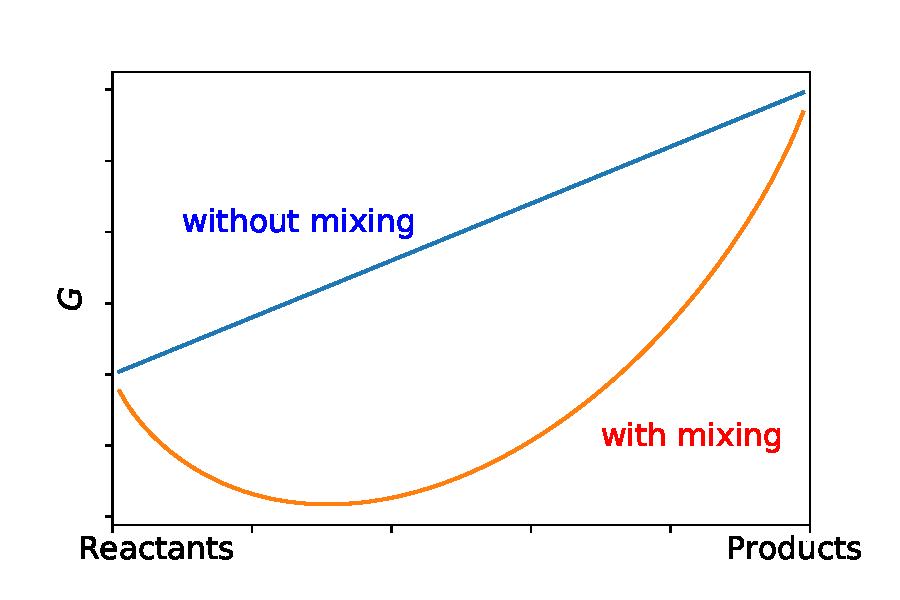
\includegraphics[width=10cm]{imgs/Reaction.pdf}
\caption{The free energy plot as a function of the extent of the chemical reaction. }
\end{figure}


We can characterize the equilibrium point by the condition that the slope of $G$ is zero. Therefore,
\begin{equation} 
0 = dG = \sum_i \mu_i dN_i
\end{equation} 

This actually tells us the chemical potentials must be satisfied at equilibrium.

{\bf exercise} Write down the equilibrium condition for each of the following reactions.
\begin{enumerate}
\item \ce {2H <-> H2}
\item \ce {N2 + 3H2 <-> 2NH3}
\item \ce {2CO + O2 <-> 2CO2}
\item \ce {CH4 + 2O2 <-> 2H2O + CO2}
\end{enumerate}

\section{Nitrogen Fixation}
Let's investigate a reaction in more details. The reaction that N$_2$ and H$_2$ combine to form ammonia is called nitrogen fixation
because it puts the nitrogen into a form that can be used by plants to synthesize amino acids and other important molecules.
Under the equilibrium condition, the chemical potentials must satisfy the following,
\begin{equation}
\mu^0(N_2) + kT\text{ln}\frac{P(N_2)}{P^0} + 3\mu^0(H2) + 3kT\text{ln}\frac{P(H_2)}{P^0}  =  2\mu^0(NH_3) + 2kT\text{ln}\frac{P(NH_3)}{P^0}
\end{equation}

Normally, we take $P^0$ to be 1 bar. Gathering all the $\mu^0$, we come to,
\begin{equation}
kT\text{ln}\frac{P(N_2)}{P^0} + 3kT\text{ln}\frac{P(H_2)}{P^0} - 2kT\text{ln}\frac{P(NH_3)}{P^0} = 
2\mu^0{NH_3} - \mu^0(N_2) - 3\mu^0{H_2}
\end{equation}

\begin{equation}
RT\text{ln}\frac{P(N_2)P^3(H_2)}{P^2(NH_3)(P^0)^2} = \Delta{G^0}
\end{equation}
or
\begin{equation}
\frac{P(N_2)P^3(H_2)}{P^2(NH_3)(P^0)^2} = e^{\Delta{G^0}/RT}
\end{equation}

Here we define the right side as the equilibrium constant, $K$.

\section{van't Hoff equation}
What's the temperature dependence of $K$?
\begin{equation}
\frac{d\text{ln}K}{dT} = \frac{d(-\Delta{G^0}/RT)}{dT} =  \frac{d(-\Delta{H^0-TS}/RT)}{dT} = \frac{\Delta{H^0}}{RT^2}
\end{equation}
If $\Delta{H^0}$ is positive, then higher temperature is needed to make the reaction tend more to the right.

Catalyst only changes the rate (kinetics) 
$P$, $T$ help to improve $K$

\section{Homework}
Problem: 5.84, 5.85



\lecture{21}{The Boltzmann Factor and Partition Function}{Qiang Zhu}{scribe-name1,2,3}


\section{Outline}
Most of the class is to deal with the second law of thermodynamics, in which we rely on the experimental measurements (of $S$, $H$) to make the
quantitative predictions. Ideally, we would like to calculate all thermodynamic quantities from first principles, starting from microscopic models
of various systems of interest, just like what we did on ideal gas and Einstein solid. For these more complicated models the direct combinatoric approach
used in \textit{Chapters 2 and 3} would be too difficult. We therefore need to develop new tools.

\section{The Boltzmann Factor}

We must start with some assumptions. All microstates should be equally probable. Let's say we have two macrostates $s_2$ and $s_2$. Their energies are $E(s_1)$ and $E(s_2)$, and their probabilities are $P(s_1)$ and $P(s_2)$, the corresponding macrostates multiplicities of the reservoir are
$\Omega_R(s_1)$ and $\Omega_R(s_2)$. The ratio of probabilities for any two states is
 
\begin{equation} \frac{P(s_2)}{P(s_1)} = \frac{\Omega_R(s_2)}{\Omega_R(s_1)} \end{equation}

Let's rewrite it in terms of $S$,

\begin{equation} \frac{P(s_2)}{P(s_1)} = \frac{e^{S_R(s2)/k}}{e^{S_R(s1)/k}} = e^{[S_R(s2)-S_R(s1)]/k} \end{equation}

According to the thermodynamic identify,
\begin{equation}
dS_R = \frac{1}{T} (dU_R + PdV_R - \mu dN_R) 
\end{equation}

For simplicity, let's again ignore $PdV$ and $\mu dN$. At atomosphere, $PdV$ is very small. $\mu dN$ contributions vary a lot. Let's throw it away for now.
\begin{equation}
dS_R = \frac{1}{T} (U_R(s_2) - U_R(s_1)) 
\end{equation}

Therefore, we have,
\begin{equation}
\frac{P(s_2)}{P(s_1)} = \frac{e^{-E(s_2)/kT}}{e^{-E(s_1)/kT}}
\end{equation}

And we define the exponential factors as {\bf Boltzmann factor}
\begin{equation}
\text{Boltzmann factor} = e^{-E(s)/kT}
\end{equation}

Now we conclude that the probability of each state is proportional to the corresponding Boltzmann factor with a scaling factor.
Let's call it 1/$Z$ for now,
\begin{equation}
P(s) = \frac{1}{Z}e^{-E(s)/kT}
\end{equation}


\begin{figure}[h]
\centering
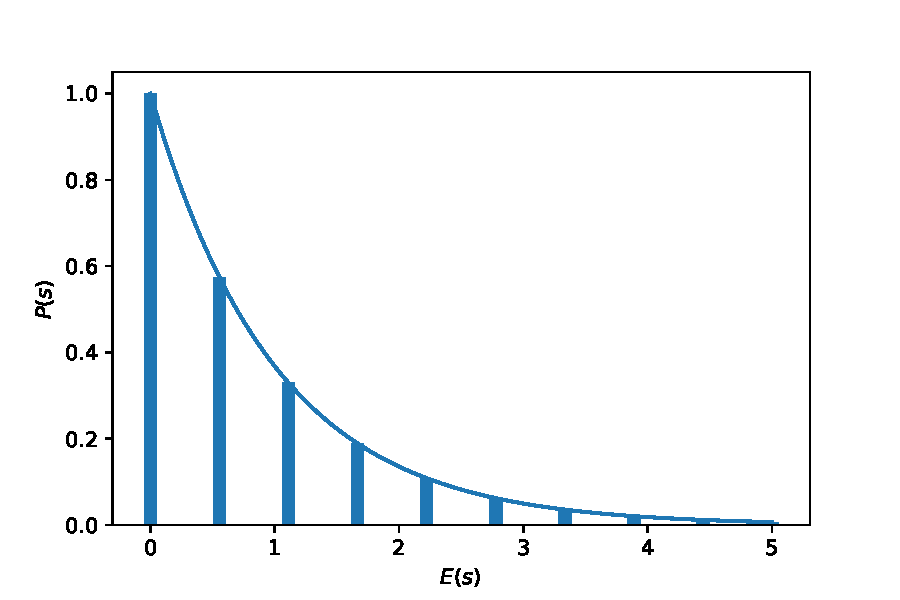
\includegraphics[width=10cm]{imgs/Boltzmann}
\caption{The probability according to the Boltzmann distribution. (1) it decays exponentially; (2) high $T$ slows down the decay. }
\end{figure}



\section{Partition Function}
Now, you are probably wondering how to calculate $Z$. The trick is to use the condition of $P(s)$,
\begin{equation}
\sum_s P(s) = \sum_s \frac{1}{Z} e^{-E(s)/kT} = \frac{1}{Z} \sum_s e^{-E(s)/kT}
\end{equation}

Hence, 
\begin{equation}
Z = \sum_s e^{-E(s)/kT}
\end{equation}

The sum is not easy to carry out numerically for most of the cases. But we can take the advantage of the exponential behavior to do it numerically.
When $E(s)$ goes to larger than a few of $kT$, the Boltzmann factor decays very fast, thus we can simply do sum for a few $kT$.

The quantity $Z$ is called {\bf partition function}. $Z$ does not depend on any particular state $s$, but it does depend on temperature. At very 
low $T$, $Z$ is approximated to 1, since all the excited states have very small Boltzmann factors. But at high temperature, $Z$ will be much larger.

{\bf Problem 6.3} Consider a hypothetical atom that has just two states, a ground state of $E$=0, and an excited state of $E$=2 eV. Draw a graph of
 the partition function for this system as a function of temperature, and evaluate the partition function numerically at $T$=[300, 3000, 30000].

\begin{figure}[h]
\centering
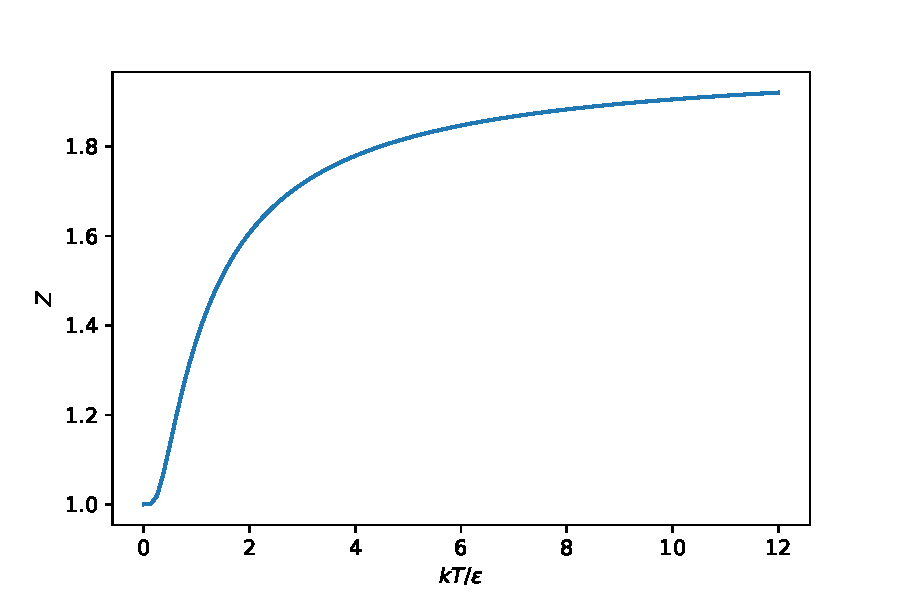
\includegraphics[width=10cm]{imgs/Partition-2s}
\caption{The partition function with respect to temperature. }
\end{figure}


\lecture{22}{Average Values and the Equipartition Theorem}{Qiang Zhu}{scribe-name1,2,3}
%\footnotetext{These notes are partially based on those of Nigel Mansell.}
% **** YOUR NOTES GO HERE:
% Some general latex examples and examples making use of the
% macros follow.  
%**** IN GENERAL, BE BRIEF. LONG SCRIBE NOTES, NO MATTER HOW WELL WRITTEN,
%**** ARE NEVER READ BY ANYBODY.

\section{Average Values}
In the previous section, we saw how to calculate the probability that a system is in any particular one of its
microstates in equilibrium with a reservoir at $T$. In the statistical mechanical systems that we are considering,
each probability is given by 
\begin{equation}
\bar{E} = \frac{1}{Z} \sum_s E(s)e^{-\beta E(s)}
\end{equation}

Similarly, the average value of any other variable of interest can be computed in the same way.
\begin{equation}
\bar{X} = \frac{1}{Z} \sum_s X(s)e^{-\beta E(s)}
\end{equation}

By using this equation, we will get the average value of any property. In statistical mechanics, we shall also
understand the fluctuations.

A very nice feature of the partition function is that 
\begin{equation}
\bar{E} = -\frac{1}{Z} \frac{\partial{Z}}{\partial{\beta}} = -\frac{\partial{\text{ln}Z}}{\partial {\beta}}
\end{equation}
when $\beta$ = 1/$kT$. These formulas can be extremely useful when you have an explicit formula for $Z$
\begin{equation}
\bar{E^2} = \frac{1}{Z} \frac{\partial^2{Z}}{\partial{\beta^2}} 
\end{equation}


\section{Rotation of Diatomic Molecules}
For a diatomic molecule, its rotational energies are quantized. The allowed rotational energies are,
\begin{equation}
E(j) = j(j+1)\epsilon
\end{equation}

where $j$ can be 0, 1, 2, etc, and $\epsilon$ is a constant that is inversely proportional to the molecule's moment of inertia.
The number of degenerate states for level $j$ is 2$j$+1. Given the energy level, we can write the partition function as a sum over $j$,
\begin{equation}
Z_\text{rot} = \sum_{j=0}^{\infty} (2j+1)e^{-E(j)/kT} = \sum_{j=0}^{\infty}(2j+1) e^{-j(j+1) \epsilon /kT}
\end{equation}
 
Unfortunately, there is no way to evaluate the sum exactly in closed form. But it is not hard to do it numerically. Even better,
we can approximate the sum as an integral that yields a very simple result.

\begin{figure}[h]
\centering
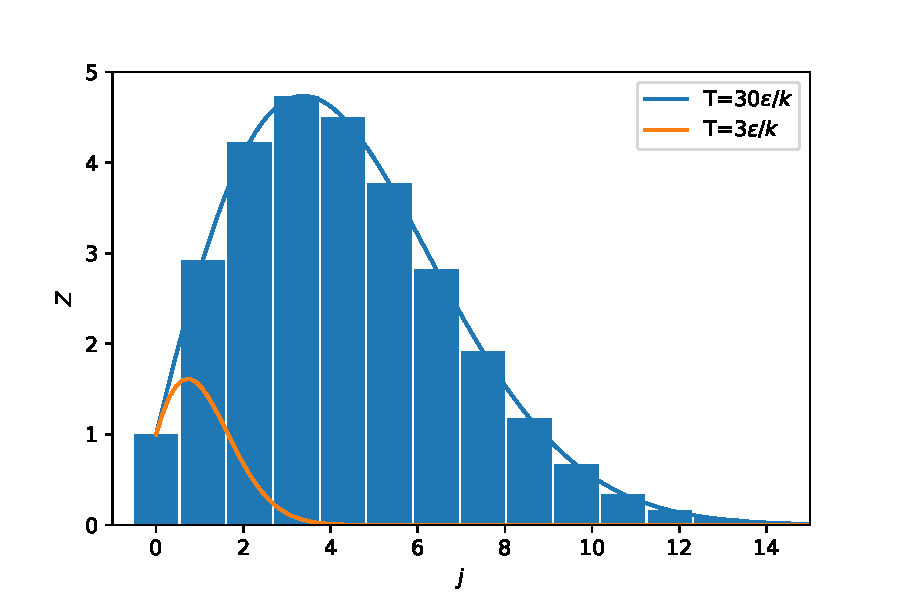
\includegraphics[width=10cm]{imgs/Rotation}
\caption{The partition sum for two different temperatures. }
\end{figure}

If we draw the curve, we could clearly see that the partition function is approximately the area under this curve at high $T$
\begin{equation}
Z_\text{rot} \approx \int_{0}^{\infty}(2j+1) e^{-j(j+1) \epsilon /kT} dj = \frac{kT}{\epsilon}  ~~~~~~~~(\text{when} ~kT >> \epsilon)
\end{equation}
 
As expected, the partition function increases when $T$ increases. For CO at room $T$, $Z_\text{rot}$ is slightly greater than 100.

With such approximation, we can then calculate the energy as well,
\begin{equation}
\bar{E}_\text{rot} = -\frac{1}{Z} \frac{\partial Z}{\partial {\beta}} 
                   = -(\beta\epsilon) \frac{\partial(1/\beta\epsilon)}{\partial{\beta}}=1/kT
\end{equation}
 
This is just the prediction of the equipartition theorem, since a diatomic molecule has two rotational degrees of freedom. 
At low temperature, the 3rd law tells us that the heat capacity must go to zero.
Above is the case of diatomic molecules made of different atoms. If it is N$_2$, 
\begin{equation}
Z_\text{rot} \approx \frac{kT}{2\epsilon}
\end{equation}
 
But this won't effect the energy and heat capacities. (problem 6.30)


\section{Equipartition Theorem}
The equipartition theorem has been extensively used in this class. However, we haven't proved it yet.
It turns out that the proof is quite easy, with the help of Boltzmann factors.

Suppose any energy term is in quadratic form, namely,
\begin{equation}
E(q) = cq^2
\end{equation}

The partition function is
\begin{equation}
Z = \sum_q e^{-\beta E(q)} = \sum_q e^{-\beta cq^2}
\end{equation}

Again, we can transform the sum to an integral
\begin{equation}
Z = \frac{1}{\Delta{q}} \int_{-\infty}^{\infty}  e^{-\beta cq^2} dq
\end{equation}

Let $x=\sqrt{\beta c}q$, so 

\begin{equation}
Z = \frac{1}{\Delta{q}\sqrt{\beta c}}\int_{-\infty}^{\infty}  e^{-x^2} dx
\end{equation}

The function $e^{-x^2}$ is called a Gaussian function.
\begin{equation}
\int_{-\infty}^{\infty}  e^{-x^2} dx = \sqrt{\pi}
\end{equation}

Therefore,
\begin{equation}
Z = \frac{1}{\Delta{q}} \sqrt{\frac{\pi}{\beta c}} = C\beta^{-1/2}
\end{equation}
where $C=\sqrt{\pi/c}/\Delta{q}$

and the energy can be readily computed,
\begin{equation}
\bar{E} = -\frac{1}{Z} \frac{\partial Z}{\partial {\beta}} = ~~~~~~~~~~~~~~~~~~~~~~~~~~~~ = \frac{1}{2}kT
\end{equation}

The limitation of the theorem is that we actually used the integral to replace the sum, which is correct when the spacing between energy level ($\epsilon$) is much less than $kT$.



\lecture{23}{Maxwell Distribution, Partition Functions and Free Energy}{Qiang Zhu}{scribe-name1,2,3}
%\footnotetext{These notes are partially based on those of Nigel Mansell.}
% **** YOUR NOTES GO HERE:
% Some general latex examples and examples making use of the
% macros follow.  
%**** IN GENERAL, BE BRIEF. LONG SCRIBE NOTES, NO MATTER HOW WELL WRITTEN,
%**** ARE NEVER READ BY ANYBODY.

\section{Maxwell Speed Distribution}
In the very first lecture, we briefly mentioned a microscopic model to link the speed of particles to the temperature,
\begin{equation} \label{PV-micro} PV = Nm{\overline v_x^2} = NkT\end{equation}

But this is just a sort of average. Technically, the speeds of particles should follow some distribution.
Let's call it as $D(v)$. What's the dependence of $D(v)$?

The first factor should be just the Boltzmann factor. 
\begin{equation}
D(v) \propto e^{E/kT} = e^{-mv^2/2kT}
\end{equation}
This only accounts for ideal gas, where the transnational motion is independent of other variables.

The second factor should be the velocity space. For a give $v$, it could be in any directions. The the space is $4\pi v^2$.
Therefore,
\begin{equation}
D(v) = C \cdot 4\pi v^2 e^{-mv^2/2kT}
\end{equation}

Where $C$ is a constant. According to 
\begin{equation}
1 = \int _0 ^{\infty} D(v)dv  = C \cdot 4\pi v^2 e^{-mv^2/2kT} dv
\end{equation}

Changing variables to $x = v\sqrt{m/2kT}$,
\begin{equation}
1 =  4\pi C (\frac{2kT}{m})^{3/2}  \int _0 ^{\infty} x^2 e^{-x^2} dx
\end{equation}

By using some trick, you can find
\begin{equation}
\int _0 ^{\infty} x^2 e^{-x^2} dx = \sqrt{\pi}/4
\end{equation}

Therefore, $C=(m/2\pi kT)^{3/2}$.

Our final results is therefore,
\begin{equation}
D(v) = (\frac{m}{2\pi kT})^{3/2}4\pi v^2 e^{-mv^2/2kT}
\end{equation}

\begin{figure}[h]
\centering
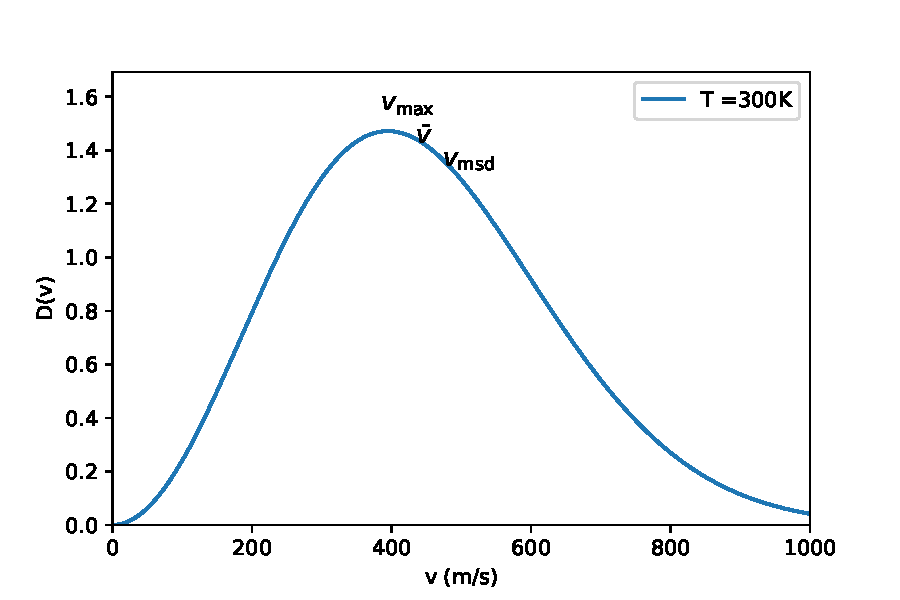
\includegraphics[width=10cm]{imgs/Maxwell-speed.pdf}
\caption{The Maxwell speed distribution and different types of characteristic speeds. }
\end{figure}




The average speed:
\begin{equation}
\bar{v} = \int _0 ^{\infty} vD(v) dv = \sqrt{\frac{8kT}{\pi m}}
\end{equation}

The rms speed:
\begin{equation}
\bar{v^2} = \int_0^{\infty} v^2D(v) dv = 3kT/m
\end{equation}

The most likely speed:
\begin{equation}
\frac{\partial D(v)}{\partial v} = 0 ~~~~\rightarrow~~~~~~ v_\text{max}= \sqrt{\frac{2kT}{m}}
\end{equation}


\section{Partition Function and Free Energy}
For a system in equilibrium with a reservoir at temperature $T$, the quantity most analogous to $\Omega$
is $Z$. Does the natural logarithm of $Z$ has some meaning?

Recall the definition of $F = U - TS$, the partial derivative with respect to $T$ is
\begin{equation}
(\frac{\partial F}{\partial{T}})_{V,N} = -S = \frac{F-H}{T}
\end{equation}

This is a differential equation for the function $F(T)$, for any given $V$ and $V$. If we use $\bar{F}$ to 
express the $kT\text{ln}Z$, then
\begin{equation}
\frac{\partial{\bar{F}}}{\partial T} = \frac{\partial}{\partial T}(-kT\text{ln}Z) = -k\text{ln}Z - kT \frac{\partial}{\partial T}\text{ln}Z
\end{equation}

In the 2nd term, we rewrite it in terms of $\beta=1/kT$
\begin{equation}
\frac{\partial}{\partial T}\text{ln}Z = \frac{\partial{\beta}}{\partial T} \frac{\partial}{\partial T}\text{ln}Z 
                                      = \frac{-1}{kT^2} \frac{1}{Z} \frac{\partial Z}{\partial {\beta}} 
                                      = \frac{U}{kT^2}
\end{equation}
Therefore,

\begin{equation}
\frac{\partial{\bar{F}}}{\partial T} = -k\text{ln}Z - kT \frac{U}{kT^2} = \frac{\bar{F}-U}{T}
\end{equation}

Therefore, $\bar{F}$ obeys the exactly same differential equation as $F$.

At $T$=0, the original $F$ is simply equal to $U$, the energy must be the lowest possible energy $U_0$, since the Boltzmann
factors for all excited states will be infinitely suppressed in comparison to the ground state. Therefore,
\begin{equation}
\bar{F}(0)= -kT\text{ln}Z(0)= U(0) = F(0)
\end{equation}

This relation could be very useful to compute entropy, pressure, and so on.
\begin{equation}
S = -(\frac{\partial{F}}{\partial{T}})_{V,N} ~~~~  P = -(\frac{\partial{F}}{\partial{T}})_{T,N} 
~~~~~~ \mu = (\frac{\partial{F}}{\partial{N}})_{V,T}
\end{equation}



\lecture{24}{Ideal Gas Model in Boltzmann Statistics}{Qiang Zhu}{scribe-name1,2,3}

\section{Partition Functions for Composite Systems}
Consider a system of just two particles, 1 and 2. If these particles do not interact with each other, there 
energy is just simply $E1$ + $E2$, then

\begin{equation}
Z_\text{total} = \sum_{s} e^{-\beta[E_1(s)+E_2(s)]} = \sum_{s} e^{-\beta E1(s)} e^{-\beta E2(s)}
\end{equation}
 
Where the sum runs over all states $s$ for the composite system. If the two particles are indistinguishable,
\begin{equation}
Z_\text{total} = \sum_{s1}\sum_{s2} e^{-\beta E1(s1)} e^{-\beta E2(s2)}
\end{equation}
 
In this case, we split the total partition functions $Z$ into to separate $Z1$ and $Z2$.
\begin{equation}
Z_\text{total} = Z_1Z_2
\end{equation}
 
If the two particles are indistinguishable, we have to apply 1/2 to reduce the double counts.
\begin{equation}
Z_\text{total} = \frac{1}{2}Z_1Z_2
\end{equation}

This formula is not precisely correct, because there are some terms {\bf in the double sum in which both particles are in the same state 
when the system is very dense}. 

Therefore, the generalization of the equation is the following
\begin{equation}
Z_\text{total} = Z_1Z_2Z_3\cdot\cdot\cdot Z_N
\end{equation}

\begin{equation}
Z_\text{total} = \frac{1}{N!}Z_1^N
\end{equation}

\section{The Partition Function of Ideal Gas}
An ideal gas should have the following partition function form,
\begin{equation}
Z_\text{total} = \frac{1}{N!}Z_1^N
\end{equation}

To calculate $Z_1$, we must make the Boltzmann factor,
\begin{equation}
e^{-E(s)/kT} = e^{-E_\text{tr}(s)/kT}  e^{-E_\text{int}(s)/kT}
\end{equation}

Since $Z$ is additive,
\begin{equation}
Z_1 = Z_\text{tr}Z_\text{int}
\end{equation}

Where
\begin{equation}
 Z_\text{tr} = \sum e^{-E_\text{tr}/kT}  ~~~~~   Z_\text{int} = \sum e^{-E_\text{int}/kT}
\end{equation}

To calculate $Z_\text{tr}$, we can start with the case of a molecule confined to a one-dimensional box.
\begin{equation}
\lambda_n = \frac{2L}{n},    ~~~~~~ n = 1,2,....,
\end{equation}

\begin{equation}
p_n = \frac{h}{\lambda_n}=\frac{hn}{2L}    ~~~~~~ n = 1,2,....,
\end{equation}

\begin{equation}
E_n = \frac{p_n^2}{2m}=\frac{h^2n^2}{8mL^2}   
\end{equation}

Therefore, 
\begin{equation}
Z_\text{1d} = \sum_n e^{-E_n/kT} = \sum e^{\frac{-h^2n^2}{8mL^2kT}}
\end{equation}

By doing integration
\begin{equation}
Z_\text{1d} = \int_0^{\infty}  e^{\frac{-h^2n^2}{8mL^2kT}} dn 
            = \frac{\sqrt{\pi}}{2} \sqrt{\frac{8mL^2kT}{h^2}} 
            = \sqrt{\frac{2\pi mkT}{h^2}}L
            = \frac{L}{L_Q}  ~~~~ (L_Q: ~\text{Quantum length})
\end{equation}

For 3 dimension, 
\begin{equation}
E_\text{tr} = \frac{p_x^2}{2m} + \frac{p_y^2}{2m} + \frac{p_z^2}{2m}
\end{equation}

\begin{equation}
Z_\text{tr} = \frac{L_x}{L_Q} \frac{L_y}{L_Q} \frac{L_z}{L_Q} = \frac{V}{V_Q} ~~~~ (V_Q: ~\text{Quantum Volume})
\end{equation}

\begin{equation}
Z_{1} = \frac{V}{V_Q} Z_\text{int}
\end{equation}

where
\begin{equation}
Z = \frac{1}{N!} (\frac{VZ_\text{int}}{V_Q})^N
\end{equation}
and
\begin{equation}
\text{ln}Z = N[\text{ln}V + \text{ln}Z_\text{int} - \text{ln}N - \text{ln}V_Q + 1]
\end{equation}


Knowing $Z$ can help us to compute many quantities,
\begin{equation}
U = -\frac{1}{Z}\frac{\partial Z}{\partial{\beta}} = -\frac{\partial \text{ln}Z}{\partial{\beta}} 
\end{equation}
\begin{equation}
U = -N\frac{\partial \text{ln}Z_\text{int}}{\partial{\beta}} + N\frac{1}{V_Q}\frac{\partial{V_Q}}{\partial{\beta}}
  = N\bar{E}_\text{int} + N\frac{3}{2\beta} = U_\text{int} + \frac{3}{2}NkT
\end{equation}

\begin{equation}
C_V = \frac{\partial U}{\partial T} =  \frac{\partial{U_\text{int}}}{\partial{T}} + \frac{3}{2}Nk
\end{equation}

\begin{equation}
F = -kT\text{ln}Z = -NkT[\text{ln}V - \text{ln}N - \text{ln}V_Q + 1] + F_\text{int}
\end{equation}

From this, it is easy to compute 
\begin{equation}
P = -(\frac{\partial F}{\partial V})_{T,N}  = \frac{NkT}{V}
\end{equation}




\lecture{25}{Gibbs Factor, Bosons, Fermions}{Qiang Zhu}{scribe-name1,2,3}


\section{The Gibbs Factor}
Remember when deriving the Boltzmann factor in the previous chapter, we wrote the ratio of probabilities of 
two different states as follows,
\begin{equation} 
\frac{P(s_2)}{P(s_1)} = \frac{\Omega_R(s_2)}{\Omega_R(s_1)} 
                      = \frac{e^{S_R(s_2)/k}}{e^{S_R(s_2)/k}}
                      = e^{[S_R(s_2)-S_R(s_1)]/k}
\end{equation}

According to the thermodynamic identify,
\begin{equation}
dS_R = \frac{1}{T} (dU_R + PdV_R - \mu dN_R) 
\end{equation}

When constructing the Boltzmann factor, we ignored $PdV$ and $\mu dN$ terms. However, we want to keep the  $\mu dN$ to account
for the exchanges in the number of particles. 
\begin{equation}
\frac{P(s_2)}{P(s_1)} = \frac{e^{[-E(s_2)-\mu N(s_2)]/kT}}{e^{[-E(s_1)-\mu N(s_1)]/kT}}
\end{equation}

And here we call the exponential factor Gibbs factor.

Accordingly, the probability functions is written as
\begin{equation}
P(s) = \frac{1}{Z}e^{-E(s)/kT}
\end{equation}

Where $Z$ is called the grand partition function
\begin{equation}
Z = \sum e^{[-E(s)-\mu N(s)]/kT}
\end{equation}

If more than one type of particle can be present, the $\mu dN$ term becomes $\sum {\mu_i dN_i}$

The grand partition is very useful in dealing with situation where the particles exchange during the process.


\section{Bosons and Fermions}
More importantly, the concept of Gibbs factors is very useful in quantum statistics, the study of dense systems in which two
or more identifcal particles have reasonable chance to occupy the same single-particle state.

Bosons: phontons, helium-4, integer spin

Fermions: electrons, protons, neutrons, half-integer spin.

When the system is very dense, namely $Z1 \gg N$, this becomes important.
Quantum length/volume.

\section{The Distribution Functions}
\begin{equation}
P(n) = \frac{1}{Z}e^{-(n\epsilon-\mu n)/kT} = \frac{1}{Z} e^{-n(\epsilon-\mu/kT}
\end{equation}

If the particles are fermions, $n$ could be only 0 or 1, so the grand partition function becomes
\begin{equation}
Z = 1 + e^{-(\epsilon-\mu)/kT}
\end{equation}

And the average number of particles is
\begin{equation}
\begin{split}
\bar{n} = \sum_n{nP(n)} &= 0\cdot P(0) + 1\cdot P(1) \\
                        &= \frac{e^{-(\epsilon-\mu)/kT}}{1+e^{-(\epsilon-\mu)/kT}}\\
                        &= \frac{1}{e^{-(\epsilon-\mu)/kT}+1}
\end{split}
\end{equation}


If the particles are Bosons,
\begin{equation}
\begin{split}
Z   & = 1 + e^{-(\epsilon-\mu)/kT} + e^{-2(\epsilon-\mu)/kT} + ...\\
    & = 1 + e^{-(\epsilon-\mu)/kT} + (e^{-(\epsilon-\mu)/kT})^2 + ...\\
    & = \frac{1}{1- e^{-(\epsilon-\mu)/kT}}
\end{split}
\end{equation}

and
\begin{equation}
\bar{n} = \sum_n{nP(n)} = 0\cdot P(0) + 1\cdot P(1) + ....
\end{equation}

Similar to what we did on $\bar{E}$, let $x = (\epsilon-\mu)/kT$,
\begin{equation}
\bar{n} = \sum_n{n \frac{e^{-nx}}{Z}} = -\frac{1}{Z} \sum{\frac{\partial e^{-nx}}{\partial x}} = -\frac{1}{Z}\frac{\partial Z}{\partial x}
\end{equation}

Therefore,
\begin{equation}
\begin{split}
\bar{n} & = -\frac{1}{1-e^{-x}}\frac{\partial (1-e^{-x})^{-1}}{\partial x} = \\
        & = \frac{1}{e^{(\epsilon-\mu)/kT}-1}
\end{split}
\end{equation}

For the classical particles,
\begin{equation}
P(s) = \frac{1}{Z} e^{-\epsilon/kT}
\end{equation}
and
\begin{equation}
\bar{n} = NP(s) = \frac{N}{Z1}e^{\epsilon/kT}
\end{equation}
According to the result of Problem 6.44, the chemical potential for such system is
\begin{equation}
\mu = -kT\textrm{ln}(Z_1/N)
\end{equation}
\begin{equation}
\bar{n} = NP(s) = \frac{N}{Z1}e^{\epsilon/kT}=e^{\mu/kT}e^{\epsilon/kT} = e^{-(\epsilon-\mu)/kT}
\end{equation}


Show the plots of $n$ versus $\epsilon$ for Bosons, Fermions and Boltzmann particles.
Clearly, the three distributions become equal when $(\epsilon-\mu)/kT \gg 1$.
For any of these applications, we can apply the distributions as long as we know the chemical potential.



\lecture{26}{The Einstein and Debye Models of Solids}{Qiang Zhu}{scribe-name1,2,3}

\section{Einstein Model}
The Einstein Model of a solid crystal is expressed as an independent three dimensional harmonic oscillator.
The multiplicity of an Einstein solid containing $N$ oscillators and $q$ energy units is approximately
\begin{equation} 
\Omega(N, q) \approx (\frac{q+N}{q})^q (\frac{q+N}{N})^N
\end{equation}
Starting with this formula, the entropy could be expressed as 
\begin{equation} 
\begin{split}
S = k\textrm{ln}\Omega &= k\textrm{ln}(\frac{q+N}{q})^q + k\textrm{ln}(\frac{q+N}{N})^N\\
                       &= kq\textrm{ln}(\frac{q+N}{q}) + kN\textrm{ln}(\frac{q+N}{N})
\end{split}
\end{equation}

Let us express the energy as $U = q\epsilon$ 
\begin{equation}
\begin{split}
\frac{1}{T} &= \frac{\partial S}{\partial U} = \frac{1}{\epsilon}\frac{\partial S}{\partial q} \\
            &= \frac{k}{\epsilon} \frac{\partial}{\partial q}[q\textrm{ln}(q+N) - q\textrm{ln}q + N\textrm{ln}(q+N) - N\textrm{ln}N] \\
            &= \frac{k}{\epsilon} [\textrm{ln}(q+N) + \frac{q}{q+N} - \textrm{ln}q  - \frac{q}{q} +  \frac{N}{q+N} + 0] \\
            &= \frac{k}{\epsilon} [\textrm{ln}\frac{q+N}{q} + \frac{q+N}{q+N} - \frac{q}{q}] \\
            &= \frac{k}{\epsilon} \textrm{ln}\frac{q+N}{q} 
\end{split}
\end{equation}
So the $U$ can be expressed as follows
\begin{equation}
U = \frac{N\epsilon}{e^{\epsilon/kT}-1}
\end{equation}

The heat capacity is therefore
\begin{equation}
C_V =  \frac{\partial U}{\partial T} 
    = -\frac{N\epsilon}{(e^{\epsilon/kT}-1)^2} \frac{\partial e^{\epsilon/kT}}{\partial T} 
    =  \frac{N\epsilon^2}{kT^2} \frac{e^{\epsilon/kT}}{(e^{\epsilon/kT}-1)^2}
    =  Nk \frac{ (\epsilon/kT)^2  e^{\epsilon/kT}}{(e^{\epsilon/kT}-1)^2}
\end{equation}

When $kT \gg \epsilon$,
\begin{equation}
C_V = \frac{N\epsilon^2}{kT^2} \frac{1+ \epsilon/kT} {(\epsilon/kT)^2} = Nk
\end{equation}
Remember we would have 3$N$ oscillators for $N$ atoms, therefore $C_V = 3Nk$.
This exactly follows the equipartition theorem. 

Below $kT \approx \epsilon$, the heat capacity falls off, approaching zero as the temperature goes to zero. This prediction generally agrees with experiment but not in detail. The equation predicts $C_V$ exponentially goes to 0, when T $\rightarrow$ 0. But experiments show that the true low-temperature behavior is cubic: $C_V \propto T^3$. The problem with the Einstein model is that the atoms in a crystal do not vibrate independently of each other. Therefore a better assumption is needed.

\section{Debye Model}
In reality, there should be low-frequency modes of oscillation in which large groups of atoms are moving together, and also high-frequency modes in which atoms are moving opposite to their neighbors.
The units of energy come in different sizes, proportional to the frequency of the modes of the vibration. Even at very low temperatures, a few low-frequency modes are still active. 
This is the reason why the heat capacity goes to 0 less dramatically than the prediction by the Einstein model.

Based on this reasoning, Debye proposed that each mode of oscillation has a set of equally spaced energy levels with the unit of energy equal to
\begin{equation}
\epsilon = hf = \frac{hc_s}{\lambda}=\frac{hc_sn}{2L}
\end{equation}
Where $L$ is the length of crystal, $n$ is the magnitude of the vector in $n$-space specifying the shape of the wave, and $c_s$ is the speed of the wave.

When the mode is in equilibrium at temperature $T$, the number of units of energy is given by the Plank distribution:
\begin{equation} 
\bar{n} = \frac{1}{e^{\epsilon/kT}-1}
\end{equation} 
We can think of these units of energy as particles obeying the Bose-Einstein statistics with $\mu$=0. These particles are called {\emph phonons}.

To calculate the total thermal energy, we add up the energies of all allowed modes:
\begin{equation}
U = 3\sum_{n_x}\sum_{n_y}\sum_{n_z} \epsilon \bar{n}(\epsilon)
\end{equation}
The factor of 3 counts the three polarization states for each polarization states for each $\bar{n}$.

In a crystal, the atomic spacing puts a strict lower limit on the wavelength. $n$ cannot exceed the number of atoms in a row. If the 3D crystal 
is a cube, the $n$ along any direction is $N^{\frac{1}{3}}$, where $N$ is the total volume.

Summing over a cube depends on $n_x$, $n_y$ and $n_z$ in a very complicated way. Debye got the idea to pretend that the relevant region of $n$-space is 
a sphere. He chose a sphere whose total volume is $N$. You can easily show that the radius of the sphere has to be
\begin{equation}
n_\textrm{max} = (\frac{6N}{\pi})^{1/3}
\end{equation}

Physical explanations:
\begin{enumerate}
\item At high $T$, only the total number of modes matters.
\item At low $T$, modes with large $\bar{n}$ are frozen out anyway.
\item In the intermediate region, not exact, but a continuous function.
\end{enumerate}

Therefore, we apply the Debye's approximation and convert the sums to integrals in spherical coordinates,
\begin{equation}
U = 3 \int_0^{n_\textrm{max}} dn \int_0^{\pi/2} d\theta \int_0^{\pi/2} d\phi n^2\textrm{sin}\theta \frac{\epsilon}{e^{\epsilon/kT}-1}
\end{equation}
Since the angular integrals gives $\pi/2$, leaving us with
\begin{equation}
U = \frac{3\pi}{2} \int_0 ^{n_\textrm{max}} \frac{hc_s}{2L} \frac{n^3}{e^{hc_sn/2LkT}-1} dn
\end{equation}

Let's make a substitution,
\begin{equation}
x = \frac{hc_sn}{2LkT}
\end{equation}

Then 
\begin{equation}
x_\textrm{max} = \frac{hc_s n_{\textrm{max}}}{2LkT} = \frac{hc_s}{2kT} (\frac{6N}{\pi V})^{1/3} = \frac{T_D}{T}
\end{equation}
$T_D$ is the Debye Temperature, a characteristic temperature. 

After substitution, we get
\begin{equation}
U = \frac{9NkT^4}{T_D^3} \int _0 ^{T_D/T} \frac{x^3}{e^x -1} dx
\end{equation}

When $T \gg T_D$, the upper limit of the integral is much less than 1, so $x$ is always very small, and we 
can approximate $e^x \approx 1+x$. Then 1 cancels, and the integral is simply $x^2dx$, leading to the final result
\begin{equation}
 U = \frac{9NkT^4}{T_D^3} \frac{1}{3} (\frac{T_D}{T})^3 = 3NkT
\end{equation}

When $T \ll T_D$, the upper limit goes to infinity, and the integral gives a constant of $\pi^4/15$, so the total energy is
\begin{equation}
U = \frac{3\pi^4}{5} \frac{NkT^4}{T_D^3}
\end{equation}
And the heat capacity becomes proportional to $T^3$.

The prediction agrees very well with low-temperature observations. However, for metal there is linear contribution from the conduction electrons.
\begin{equation}
C = \gamma T + \frac{12\pi^4Nk}{5T_D^3} T^3,
\end{equation}

where $\gamma$ is a dimensionless coefficient. The Debye temperature ranges from 88 K for lead to 1860 K for diamond. Since the heat capacity reaches 95 of its maximum value at $T=T_D$, the Debye
temperature gives you a rough idea of when you can get away with just using the equipartition theorem. 

The Debye model gives you a rough idea still. For a more rigorous analysis, one needs to know exactly the distribution of phonons, which belongs
to a book in solid state physics.

\section{Further Discussions}
\begin{enumerate}
\item{Both Einstein and Debye models give the correct high temperature limit. It indicates that all oscillators under high $T$ essentially have the same energy, even though the oscillators follow that Bose-Einstein distribution in the Debye model. Try to apply the distribution model to prove it.}
\item{In low temperature limit, the Debye model captures the right physics, but why does it fail in the intermediate temperature? In the Debye model, it assumes that the
oscillators with lower frequencies have more populations, and the phonon numbers monotonically decrease with the increase of frequency. Not true in reality!}


\begin{figure}[h]
\centering
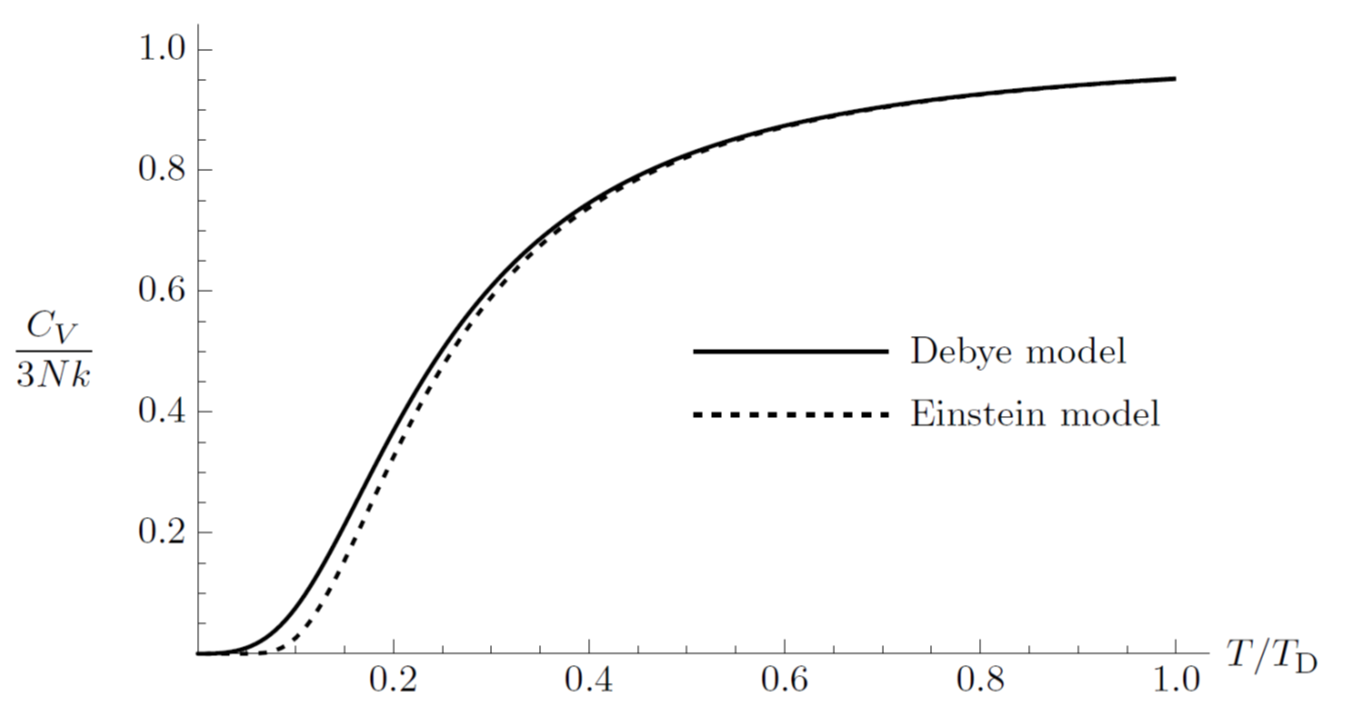
\includegraphics[width=0.9\linewidth]{imgs/Debye.png}
\caption{The Debye prediction for the heat capacity of a solid, with the
prediction of the Einstein model plotted for comparison. The constant ⇤ in the
Einstein model has been chosen to obtain the best agreement with the Debye
model at high temperatures. Note that the Einstein curve is much flatter than the Debye curve at low temperatures. Copyright 2000, Addison-Wesley. }
\end{figure}

\end{enumerate}




\lecture{27}{Free Electron Gases}{Qiang Zhu}{scribe-name1,2,3}

\section{The Regime of Quantum Statistics}
As said in the introduction of Fermions and Bosons, Quantum Statistics starts to play the role in the dense system and low temperatures.
For an electron at room temperature, the quantum volume is
\begin{equation}
V_Q = (\frac{h}{\sqrt{2\pi mkT}})^3 = (\textrm{4.3~nm})^3
\end{equation}

In a typical metal, there is about one (or two) conduction electron per atom, the volume per electron is roughly the volume of
an atom, namely $(\textrm{0.2 nm})^3$. Therefore, the temperature regime for electron has a pretty wide range. 
In other word, the temperature is much too low for Boltzmann statistics to apply.

In the following, we will exclusively discuss the case of electron, a typical Fermion at zero and above temperature.

\section{Electron at 0 K}
At $T$ = 0, the Fermi-Dirac distribution becomes a step function. All single-particle with energy less than $\mu$ are occupied, while
all states with energy greater than $\mu$ are unoccupied. Here we call $\mu$ \textbf{Fermi energy} $\epsilon_F$.

In order to calculate $\epsilon_F$, as well as other properties such as the total energy and the pressure of the electron gas,
let's make the approximation that the electrons are free particles, subject to no external forces. 
This is almost for metal accurate expect that there still exists the attractive forces from nearby ions in the crystal lattice.

The definite energy wavefunctions of a free electron inside a box are just sine waves. For a one-dimensional box the allowed wavelengths and momentas are
\begin{equation}
\lambda_n = \frac{2L}{n}, ~~~~~~~~~~~ p_n = \frac{h}{\lambda_n} = \frac{hn}{2L}
\end{equation}
where $n$ is any positive integer. In a three dimensional box these equations apply separately to each direction, so
\begin{equation}
\epsilon = \frac{p^2}{2m} = \frac{h^2}{8mL^2}(n_x^2+n_y^2+n_z^2)
\end{equation}

These allowed states will form a series of eighth-spheres in the 3D space. And the radius of the largest sphere will be $\epsilon_F$,
\begin{equation}
\epsilon_F = \frac{h^2n_\textrm{max}^2}{8mL^2}
\end{equation}

The total volume of the eighth-sphere equals the number of lattice points enclosed. Therefore the total number of occupied states is
twice this volume,
\begin{equation}
N = 2 \cdot \frac{1}{8} \cdot \frac{4}{3} \pi n_\textrm{max}^3 = \frac{\pi n_\textrm{max}^3}{3}
\end{equation}

To calculate the total energy of all electrons, we need to sum over the energies of the electrons in all occupied states.
\begin{equation}
U = 2 \sum_{n_x} \sum_{n_y} \sum_{n_z} = 2 \int\int\int \epsilon(n) dn_x dn_y dn_z.
\end{equation}

The factor of 2 is for the two spin orientations for each $n$. 
Transforming the triple integral to the spherical coordinates, we have the total energy as follows,
\begin{equation}
U = 2 \int_0^{n_\textrm{max}} dn \int_0 ^{\pi/2} d\theta \int_0 ^{\pi/2} d\phi n^2 \textrm{sin}\theta \epsilon(n)
\end{equation}

The angular integrals give $\pi/2$, which leaves us with
\begin{equation}
U = \pi \int_0^{n_\textrm{max}} n^2 \epsilon(n) dn 
  = \frac{\pi h^2}{8mL^2} \int _0 ^{n_\textrm{max}} n^4 dn
  = \frac{\pi h^2 n^5_\textrm{max}}{40mL^2} 
  = \frac{3}{5} N \epsilon_F
\end{equation}

The Fermi energy for conduction electrons in a typical metal is a few eVs.
We can therefore define the Fermi temperature as
\begin{equation}
T_F = \epsilon_F/k
\end{equation}

Fermi temperature is purely hypothetical for electrons in a metal, since metals liquefy or evaporate long before it is reached.
The pressure of an electron gas is
\begin{equation}
P = \frac{\partial}{\partial V} [\frac{3}{5}N \frac{h^2}{8m} (\frac{3N}{/pi})^{2/3} V^{-2/3}] 
  = \frac{2N\epsilon_F}{5V} = \frac{2U}{3V}
\end{equation}

This is called degeneracy pressure, which keeps matter from collapsing under the huge electrostatic forces that try to pull electrons and protons together.

A more measurable quantity is the bulk modulus,
\begin{equation}
B = -V (\frac{\partial P}{\partial V})_T = \frac{10U}{9V} 
\end{equation}

This quantity agrees with experiment within a factor of 3 or so, for most metals.

\section{Small Nonzero Temperature}
If we go beyond 0 K, we can calculate even more properties related to temperature. At temperature $T$, all particles typically acquire a thermal energy of $kT$.
However, in a degenerate electron gas, most of the electrons cannot obtain these energies, because all states have been already occupied. 
The only active electrons are those which are already within about $kT$ of the Fermi energy. The number is proportional to $NkT$
Thus, the additional energy that a degenerate electron gas acquires when its temperature is raised from zero to T is proportional to $N(kT)^2$.

The total energy increase would be 
\begin{equation}
 U = \frac{3}{5} N \epsilon_{F} + \frac{\pi^2}{4} N \frac{(kT)^2}{\epsilon_{F}}
\end{equation}
Therefore, the heat capacity is
\begin{equation}
C_V = (\frac{\partial U}{\partial T})_V = \frac{\pi^2Nk^2T}{2\epsilon_F}
\end{equation}

To better visualize the behavior of a Fermi gas at small nonzero $T$, we need to introduce a variable to describe the distribution of electrons with respect to the energy,
\begin{equation}
U = \pi \int_0^{n_\textrm{max}} n^2 \epsilon(n) dn 
  = \int _0 ^{\epsilon_F} \epsilon[\frac{\pi}{2} (\frac{8ml^2}{h^2}) ^{3/2} \sqrt{\epsilon}] d\epsilon
\end{equation}

The term in the square brackets is called density of states,
\begin{equation}
g(\epsilon) = \frac{\pi}{2} (\frac{8ml^2}{h^2}) ^{3/2} \sqrt{\epsilon} = \frac{3N}{2\epsilon_F^{2/3}} \sqrt{\epsilon}
\end{equation}

So $g(\epsilon)$ is proportional to $\sqrt{\epsilon}$. In a more realistic model, we would want to consider the attraction of electrons with the ions.
Then the wavefunctions and energies would be much more complicates, $g(\epsilon)$ would be very different.

For an electron gas at 0 K, we can get the total number of electrons by just integrating the density of states up to the Fermi energy
\begin{equation}
N = \int_0 ^{\epsilon_{F}} g(\epsilon) ~~~~~ (T=0)
\end{equation}

What to do with the finite temperature? We need to multiply $g(\epsilon)$ by the probability of a state by the Fermi-Dirac distribution.
\begin{equation}
N = \int_0 ^\infty g(\epsilon) \frac{1}{e^{(\epsilon-u)/kT)+1}} d\epsilon
\end{equation}

And the total energy could be expressed as 
\begin{equation}
U = \int_0 ^\infty \epsilon g(\epsilon) \frac{1}{e^{(\epsilon-u)/kT)+1}} d\epsilon
\end{equation}

Instead of falling immediately to zero at $\epsilon = \epsilon_F$, the number of electrons per unit energy now drops more gradually, over a width of a few times $kT$.
It is important to note that the Fermi energy will shift a bit with temperature.

%\section{Sommerfield Expansion}
%How to evaluate the integral? It is to find the chemical potential and total energy of a free electron gas, which was firstly introduced by Sommerfeld.
%For the integral for N:
%\begin{equation}
%N = \int_0^\infty g(\epsilon)\bar{n}_{\textrm{FD}}d\epsilon = g_0 \int_0 ^{\infty} \epsilon^{1/2} \bar{n}_{\textrm{FD}}d\epsilon
%\end{equation}
%
%Although this integral goes over all positive $\epsilon$, the most interesting region is near $\epsilon = \mu$, where $\bar{n}(\epsilon)$ falls off steeply.
%The first trick is to integrate by parts:
%\begin{equation}
%N = \frac{2}{3} g_0 \epsilon^{3/2} \bar{n}(\epsilon) %|_0^{\intfy} %+ \frac{2}{3} g_0 \int_0 ^{\infty} \epsilon^{3/2} (-\frac{d\bar{n}}{d\epsilon}) d\epsilon
%\end{equation}
%
%The boundary term vanishes at both limits, leaving us with an integral that is much nicer. Explicitly, we can compute
%\begin{equation}
%-\frac{d\bar{n}}{d\epsilon} = -\frac{d}{d\epsilon} (e^{(\epsilon-\mu)/kT}+1)^{-1} = \frac{1}{kT} \frac{e^x}{(e^x+1)^2}
%\end{equation}
%
%where $x=(\epsilon-\mu)/kT$. Thus the integral is
%\begin{equation}
%\begin{split}
%N = &\frac{2}{3}g_0 \int_0^{\infty} \frac{1}{kT} \frac{e^x}{(e^x+1)^2} \epsilon^{3/2}d\epsilon\\ 
%  = &\frac{2}{3}g_0 \int_{-\mu/kT}^{\infty}  \frac{e^x}{(e^x+1)^2} \epsilon^{3/2}d\epsilon \\
%  = &\frac{2}{3}g_0 \int_{-\infty}^{\infty}  \frac{e^x}{(e^x+1)^2} [\mu^{3/2} + 3/2xkT\mu^{1/2} + 3/8(xkT)^2\mu^{-1/2} + ... ] dx 
%\end{split}
%\end{equation}
%
%Where we expand the function $\epsilon^{3/2}$ in a Taylor series
%\begin{equation}
%\begin{split}
%\epsilon^{3/2} &= \mu^{3/2} + (\epsilon-\mu) \frac{d}{d\epsilon} \epsilon^{3/2} + \frac{1}{2}(\epsilon-\mu)^2 \frac{d^2}{d\epsilon^2} \epsilon^{2/3} + ....\\
%               &= \mu^{3/2} + \frac{2}{3}(\epsilon-\mu)\mu^{1/2} + \frac{3}{8}(\epsilon-\mu)^2 \mu^{-1/2} + ....
%\end{split}
%\end{equation}
%
%The first term is
%\begin{equation}
% N = \int_{-\infty}^{\infty}  \frac{e^x}{(e^x+1)^2} dx = \int_{-\infty}^{\infty} -\frac{d}{dx} \frac{1}{e^x+1} dx = 1
%\end{equation}
%
%The second term is 
%\begin{equation}
% N = \int_{-\infty}^{\infty}  \frac{xe^x}{(e^x+1)^2} dx = \int_{-\infty}^{\infty} \frac{x}{(e^x+1)(e^{-x}+1)} = 0.
%\end{equation}
%
%The second term is 
%\begin{equation}
% N = \int_{-\infty}^{\infty}  \frac{x^2e^x}{(e^x+1)^2} dx = \frac{\pi}{3}
%\end{equation}
%
%Therefore, we get
%\begin{equation}
%N = \frac{}{}
%\end{equation}






\lecture{28}{Bose-Einstein Condensation}{Qiang Zhu}{scribe-name1,2,3}

\section{The statistical behavior for Bosons}
As stated in the introduction to Fermions and Bosons, quantum statistics starts to play a role in dense system and low temperatures. For an atom at room temperature, the quantum volume is
\begin{equation}
\epsilon_0 = \frac{h^2}{8mL^2}(1^2+1^2+1^2) = \frac{3h^2}{8mL^2}
\end{equation}

\begin{equation}
N_0 = \frac{1}{e^{(\epsilon_0-\mu)/kT}-1}
\end{equation}

When $T$ is very small, $N_0$ will be quite large. In this case, the denominator must be small,

\begin{equation}
N_0 = \frac{1}{1+(\epsilon_0-\mu)/kT-1} = \frac{kT}{\epsilon_0-\mu}  ~~~~(\textrm{when~} N_0 \gg 1)
\end{equation}

The chemical potential $\mu$ must be equal to $\epsilon_0$ at T=0, and just a bit less than $\epsilon_0$ at small $T$. %To calculate the total energy of all electrons, we need to sum over the energies of the electrons in all occupied states. 
Now the question is \textbf{at which temperature we can observe that $N_0$ remains very large?}


\section{Computing the total number of Bosons}
\begin{equation}
N = \sum_s \frac{1}{e^{(\epsilon_s-\mu)/kT}-1}
\end{equation}

In practice, we can turn it to an integral,
\begin{equation}
\label{eq0}
N = \int_0^\infty g(\epsilon)\frac{1}{e^{(\epsilon_s-\mu)/kT}-1}d\epsilon
\end{equation}

Where $g(\epsilon)$ is the density of states, which has a similar form following the electron gas model. 
\begin{equation}
g(\epsilon) = \frac{2}{\sqrt{\pi}}\bigg(\frac{2\pi m}{h^2}\bigg)^{3/2}V\sqrt{\epsilon}
\end{equation}

\begin{figure}[h]
\centering
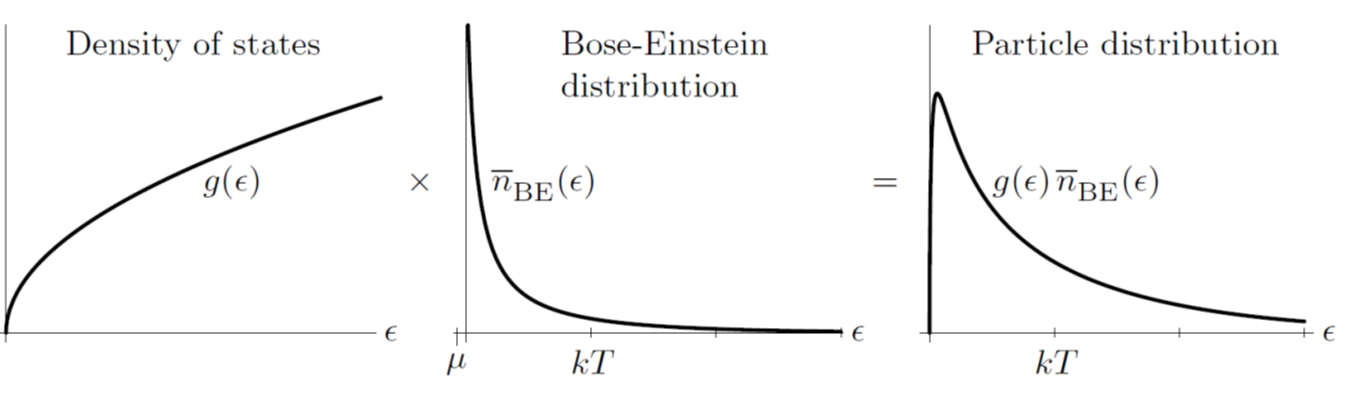
\includegraphics[width=0.9\linewidth]{imgs/BEC1.png}
\caption{The distribution of bosons as a function of energy is the product of
two functions, the density of states and the Bose-Einstein distribution. Copyright 2000, Addison-Wesley. }
\end{figure}

The trouble is that we cannot evaluate eq.(\ref{eq0}) analytically. In order to work it out, we must guess some value for the $\mu$ term. A good starting point is let $\mu$=0. Changing the variable to $x = \epsilon/kT$
\begin{equation}
\begin{split}
    N = & \frac{2}{\sqrt{\pi}}\bigg(\frac{2\pi m}{h^2}\bigg)^{3/2}V \int_0^{\infty} \frac{\sqrt{\epsilon} d\epsilon}{e^{\epsilon/kT}-1}\\
      = & \frac{2}{\sqrt{\pi}}\bigg(\frac{2\pi mkT}{h^2}\bigg)^{3/2}V \int_{0}^{\infty} \frac{\sqrt{x} dx}{e^x-1}\\
\end{split}
\end{equation}

The integral over $x$ gives 2.315, which leaves us with
\begin{equation}
N = 2.612\bigg(\frac{2\pi mkT}{h^2}\bigg)^{3/2}V
\end{equation}

That result is wrong! It means that the number of particles purely depends on $T$. In fact, there can be only one $T$ corresponds to this value.
\begin{equation}
    N = 2.612\bigg(\frac{2\pi m kT_c}{h^2}\bigg)^{3/2}V
\end{equation}

When $T<T_c$, this will be no longer valid during the transformation from summation to integral. This is because the terms from $\epsilon =0$ are missing. Therefore, it should be better expressed as
\begin{equation}
    N_\textrm{exited} = 2.612\bigg(\frac{2\pi mkT}{h^2}\bigg)^{3/2}V
\end{equation}

While the gap between $N$ and $N_\textrm{exited}$ is the number of atoms in the ground state.
\begin{equation}
    N_0 = N-N_\textrm{exited} = \bigg[1-\bigg(\frac{T}{T_c}\bigg)^{3/2}\bigg]N
\end{equation}

\begin{figure}[ht]
\centering
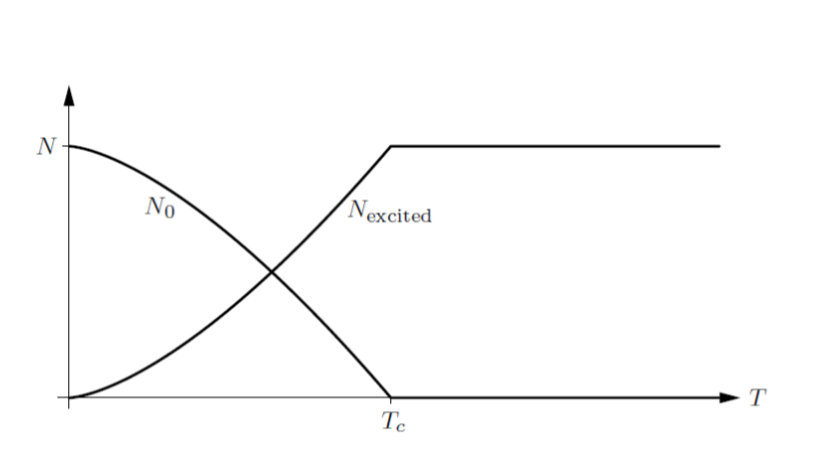
\includegraphics[width=0.8\linewidth]{imgs/BEC2.png}
\caption{Number of atoms in the ground state ($N_0$) and in excited states,
for an ideal Bose gas in a three-dimensional box. Below $T_c$ the number of atoms in excited states is proportional to $T^{3/2}$. Copyright 2000, Addison-Wesley}
\end{figure}

The abrupt accumulation of atoms in the ground state below $T_c$ is called \textbf{Bose-Einstein condensation}.

\section{Real World Examples}
In 1995 BEC of a gas of weakly interacting atoms was first achieved using Rb-87. Later, BEC was achieved with dilute gases of atomic Li, Na, H, .etc.

The superfluid phase of $^4$He is also considered to be an example of BEC.

\section{Why does it happen?}




\end{document}
